
\section{Introduction}
	Impedance spectroscopy, introduced in \cpageref{characterization_impedance}, is a powerful technique for characterising electronic devices in the frequency domain.
	The first information that can be directly extracted from impedance spectroscopy is a frequency\hyp{}dependent capacitance \cite{Brus2016}.
	When studying this in perovskite solar cells, the results are of difficult interpretation \cite{Almora2018,Guillen2014}.
	A giant\index{giant capacitance} capacitance is always observed at low frequencies for illuminated devices \cite{Juarez-Perez2014,Kim2015c}.
	More rarely, also a negative capacitance\index{negative capacitance} (\textsl{i.e.}\ an inductance) has been observed in perovskite solar cell \cite{Ghahremanirad2017,Guerrero2016,Sanchez2014} and other kinds of solar cells \cite{Mora-Sero2006,Knapp2015}.
	In order to extract the individual parameters, like transport and recombination constants, the data has to be fitted using an electronic equivalent circuit \cite{Jamnik2001}.
	The components of the circuit should have a relation with the actually existing processes, so that we can relate the parameters of the electrical component with the solar cell specific internal mechanisms.
	Many complex circuits have been proposed in literature, some of them included inductors for matching the inductive behaviour \cite{Almora2018,Ghahremanirad2017,Guerrero2016}.
	Previous to 2018, these phenomena were interpreted as surface polarisation caused by a huge free charge accumulation at the interfaces due to the influence of ionic accumulation \cite{Guerrero2016,Zarazua2016a} supported by drift\hyp{}diffusion simulations \cite{Garcia-Rosell2018,Lopez-Varo2018}.
	It has to be noted that any slow process causing a change in the flowing current could result in an apparent capacitance or inductance, this could happen with degradation processes or heating \cite{Knapp2015,Shimizu2017}.
	When studying perovskite solar cells, we have to consider that the electrostatic potential arising from mobile ion redistribution controls electronic charge transfer barriers \cite{Tress2016,Pockett2017}.
	In November 2017 we started modelling impedance spectroscopy using Driftfusion software and the modules already developed for Charge Extraction simulation.
	In May 2018 we uploaded to ArXiv a pre-print which was then published in \authoryear{Moia2019} with an alternative interpretation for the giant\index{giant capacitance} capacitance: this influence of the ionic charge on the electronic processes such as recombination and can give rise to apparent capacitive behaviour.
	This effect does not involve an accumulation of an enormous amount of charge, as it was expected by a giant\index{giant capacitance} capacitance, so it cannot be described by a capacitor in the equivalent electrical circuit.
	For the inductive behaviour (negative capacitance\index{negative capacitance}) we proposed that the same influence can affect the charge injection causing a negative apparent capacitance\index{negative capacitance}.
	Additionally, we also shown that the reaction or penetration of the perovskite's mobile ions into the contact materials can also explain some inductive behaviour.
	More or less at the same time, other research groups published similar interpretations \cite{Jacobs2018,Ebadi2019}.
	Moreover, in \authoryear{Ebadi2019} the influence of ionic migration on the injection barrier is experimentally confirmed.
	We proposed that both of the effects (apparent capacitance and inductance) can be described by transistors element in the circuit, as represented in \cref{fig:diode_transistor-transistor}.
	This allows the charge to flow through an interface to not only depend on the applied voltage, like in a Schottky diode, but also on an external influence: the ionic density close to the interface.
	The influence of ionic migration on electronic transfer can be thought as an amplification of electronic current by ionic current.
	Our model not only works in the small perturbation regime employed in impedance spectroscopy, but can also explain hysteresis\index{hysteresis} in current\hyp{}voltage sweeps as shown in Fig.5 of \authoryear{Moia2019}.
	The understanding of this mechanism allows the researchers to insightfully use impedance spectroscopy on perovskite solar cells and other ionic/\-electronic interfaces (\textsl{e.g.}\ electrochemical communication between neurons in the brain \cite{Cole1956}) but could also be employed for designing new physical electronic components showing large and tunable apparent capacitance or inductance in a reduced volume.

	\paragraph{Design of the Experiment}
	Impedance spectroscopy has been initially modelled studying the current evolution after a single voltage step.
	This first rough attempt should be polished using Kramers\hyp{}Kronig relation and has not been published yet.
	In order to confirm the initial observations, the impedance spectroscopy has been implemented trying to match the actual experimental conditions.
	For this reason, the oscillating current obtained when applying an oscillating voltage has been studied separately for each frequency.
	This caused the simulation to be much slower but still doable with my laptop.
	Additionally, the phase and amplitude has been obtained mimicking the demodulation of a lock-in amplifier rather than with a sinusoidal fitting.

	\paragraph{Author contributions}
	I implemented and run the impedance spectroscopy simulation on top of Driftfusion software developed by Dr.\ Phil Calado, Dr.\ Piers RF Barnes, Mohammed Azzouzi, Benjamin Hilton, and myself.
	Dr.\ Davide Moia and Dr.\ Piers RF Barnes created the formalism and the electrical equivalent circuit.
	William Fisher and Dr. Davide Moia fitted the experimental data using fitting routines developed by Dr.\ Piers RF Barnes.
	Dr.\ Michael Stringer, Dr.\ Onkar Game, Yinghong Hu, Dr.\ David Lidzey, and Dr.\ Pablo Docampo provided excellently stable perovskite solar cells to be studied.

\section{Driftfusion software}
	Driftfusion is a modelling platform for stacked semiconductors, mostly used for solar cells.
	It estimates the profile of electrostatic potential, free electrons, free holes, and mobile ions densities over one dimension (depth into the stack) and over time.
	The semi-classical transport, continuity, and Poisson's equations are solved using Matlab's built-in Partial Differential Equation solver for Parabolic and Elliptic equations \texttt{pdepe}
	The simulation assumes static negative counter ions simulating Schottky defects \cite{Walsh2015} and positively charged mobile ions constrained into the absorber layer.
	This formalism is based on \authoryear{Nelson2003} and described in \authoryear{Calado2016} and \authoryear{Calado2018}.
	All the mentioned functions, helper code and examples of impedance spectroscopy simulations have been released on \url{https://github.com/barnesgroupICL/Driftfusion/tree/2018-EIS}.

	\paragraph{Homojunction}
	We employed the homojunction version of Driftfusion, which at the date of September 2017 was the stable and well tested release of Driftfusion.
	This means that in the presented simulations all the materials have the same band gap but can differ by other parameters: doping level (equilibrium Fermi level position), holes and electrons mobilities, permittivity, radiative and trap mediated recombination constants, traps relative energy inside the band gap, and thickness.
	This proved to be enough for simulating the influence of ionic current on the recombination current but was limited for studying their influence on the injection current.

	\paragraph{Recombination and generation}
	High rates of recombination in the contact regions are used to simulate surface recombination.
	Even if an optical model was available in Driftfusion, an uniform generation through all the absorber proven to be enough for our purposes.

	\paragraph{Boundary conditions}
	An arbitrary time dependent voltage can be applied with time\hyp{}dependent boundary conditions.
	
	
	

\section{Simulating impedance spectroscopy}

	
\begin{table}
%	\clearpage
	%\begin{table}%[h]	% longtables cannot stay inside a float, otherwise they will not break
	\begin{xltabular}[c]{1\linewidth}{@{} >{\hsize=1.6\hsize}Y >{\hsize=0.7\hsize}Y >{\hsize=0.95\hsize}Y >{\hsize=0.8\hsize}Y >{\hsize=0.95\hsize}Y >{\hsize=1\hsize}Y @{}}
		% multirow does not get the correct number of rows with tabularx
		% mycaption does not work inside xltabular
		\caption[Drift-diffusion simulation parameters.]{\textbf{Drift-diffusion simulation parameters.}
			These parameters were used for all the data simulated with the homojunction model.
			The meaning of each is described in detail in \authoryear{Calado2016}.
			The 1 sun equivalent \gls{voc} resulting from this parameters set is \SI{0.931}{\V}, the resulting \gls{jsc} is \SI{20.3}{\mA\per\square\cm}.
		}\label{table:impedance_parameters}\\[\belowcaptionskip]
		Parameter name & Symbol & \textit{p}-type & Intrinsic & \textit{n}-type & Unit\\[1mm]
		\hline
		\endfirsthead
		\multicolumn{2}{@{}l}{\ldots \small continues}\\
		\hline
		Parameter name & Symbol & \textit{p}-type & Intrinsic & \textit{n}-type & Unit \\ 
		\hline
		\endhead
		\hline
		\multicolumn{6}{r@{}}{\small continues\ldots}\\
		\endfoot
		\hline
		\endlastfoot
		Layer thickness \rule[-2ex]{0pt}{4.5ex}&			\gls{symb:d}&			200&			500&			200&			\si{\nm}			 \\
		Band gap \rule[-2ex]{0pt}{3.5ex}&	\gls{symb:Eg}&	1.6	&1.6&	1.6&	\si{\eV}\\
		Built in voltage \rule[-2ex]{0pt}{3.5ex}&	\gls{symb:VBI}&	1.3	&1.3&	1.3&	\si{\V}\\
		Relative dielectric constant \rule[-2ex]{0pt}{3.5ex}&	\gls{symb:epsilonr}&	20&	20&	20&	/ \\
		Mobile ionic defect density \rule[-2ex]{0pt}{3.5ex}&	$N_|ion|$&	0&	\num{1e19}&	0&	\si{\per\cubic\cm}\\
		Ion mobility \rule[-2ex]{0pt}{3.5ex}&	$\mu_|a|$&	/	&\num{1e-10}&	/&	\si{\square\cm\per\V\per\s}\\
		Electron mobility \rule[-2ex]{0pt}{3.5ex}&	$\mu_|n|$	&0.02&	20&	20&	\si{\square\cm\per\V\per\s}\\
		Hole mobility \rule[-2ex]{0pt}{3.5ex}&	$\mu_|p|$&	20&	20&	0.02&	\si{\square\cm\per\V\per\s}\\
		Donor doping density \rule[-2ex]{0pt}{3.5ex}&	$N_|A|$&	\num{3e17}&	/& /&	\si{\per\cubic\cm}\\
		Acceptor doping density \rule[-2ex]{0pt}{3.5ex}&	$N_|D|$&	/&	/&\num{3e17}	&	\si{\per\cubic\cm}\\
		Effective density of states \rule[-2ex]{0pt}{3.5ex}& \gls{symb:nDOS}	&	\num{1e20}&\num{1e20}&\num{1e20}&	\si{\per\cubic\cm}\\
		Band-to-band recombination rate coefficient \rule[-2ex]{0pt}{3.5ex}&	$k_|rad|$&\num{1e-12}	&\num{1e-12}&\num{1e-12}&	\si{\cubic\cm\per\s} \\
		SRH trap energy \rule[-2ex]{0pt}{3.5ex}&	$E_|t|$&	$E_|CB|-0.8$& /&	$E_|CB|-0.8$&	\si{\eV}\\
		SRH time constants \rule[-2ex]{0pt}{3.5ex}&\gls{symb:taunp}	&	\num{5e-10}&	/&	\num{5e-10}&	\si{\s}\\
		Generation rate & \gls{symb:g}&	/&	\num{2.5e21}&	/&	\si{\per\cubic\cm\per\s}\\
	\end{xltabular}
\end{table}

	\paragraph{Initial conditions}
	The solution of the electrons, holes, ions density and electrostatic concentration profiles of the device under steady state operating conditions was determined using Driftfusion core functions and the parameters listed in \cref{table:impedance_parameters}.
	This solution provided the initial conditions for the simulated impedance spectroscopy.
	Most importantly, at this step we set the illumination intensity and the DC voltage $V_|DC|$, which usually are the explored parameters.

	\paragraph{Applied voltage}
	The impedance spectroscopy simulations were performed by applying an oscillating voltage $v$ superimposed on a background bias voltage $V_|DC|$ boundary condition:

	\begin{equation}
		V = V_|DC| + v(t) = V_|DC| + v_|max| \sin(\omega t)
	\end{equation}

	$V_|DC|$ was set equal to the steady state voltage of the provided input solution (\textsl{e.g.}\ \gls{voc} for the simulations at open circuit).
	Usually, a $v_|max|$ of \SI{2}{\mV} is employed.
	This value is much smaller than the experimentally used one but very similar results are obtained when using larger perturbations (simulations with a $v_|max|$ of \SI{200}{\mV} are mentioned in \cpageref{impedance-large_perturbations}).
	The small value allowed me to obtain a computationally fast simulation without being affected by too much numerical noise.

	\paragraph{Position and time grids}
	In order to deal with the high gradients at the interfaces, a linear spatial mesh was used with a spacing of \SI{0.55}{\nm} within the approximate depletion regions of the device and \SI{2.54}{\nm} elsewhere.
	Even if the \texttt{pdepe} solver utilises an internal time grid, it outputs the data at the requested times array.
	All the stabilisations have been performed on a logarithmic time grid (\texttt{tmesh\_type}=2 in \texttt{meshgen_t}) while all the oscillating voltage simulations have been performed on a linear time grid (\texttt{tmesh\_type}=1 in \texttt{meshgen_t}).
	For the impedance simulations, 20 complete periods are simulated with 40 time points for each period.

	\paragraph{Oscillating stabilisation}
	The change from steady state to oscillating voltage does require some complete periods before reaching a stable oscillation (where the current profile is identical from one period to the next).
	As represented in \cref{fig:impedance_flowchart}, before analysing the oscillating solutions, the stabilisation is verified comparing the last time point profiles with the profiles at the half of the current simulation (so at the \nth{10} period).
	In case the stability was absent, the last time point solution has been used as a starting point for 20 more periods, until when stabilisation was ensured.
	This is mostly important for large perturbation simulations (large $v_|max|$), where the time\hyp{}averaged profiles are rather different from the steady state ones.

	\begin{SCfigure}%demodulation
		\centering
		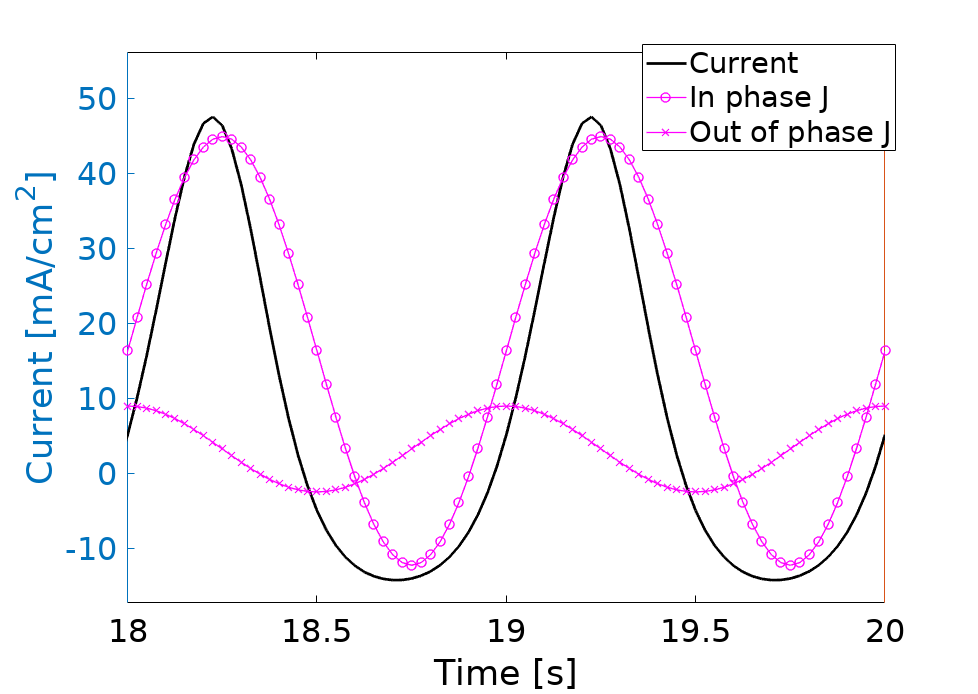
\includegraphics[width=0.65\textwidth]{demodulation/demod-result.png}
		\mycaption[Example of demodulation on a large perturbation simulation.]{
			The applied voltage is not shown, it was a sinusoidal wave with frequency \SI{1}{\Hz}.
			Black line is the simulated oscillating current, the non sinusoidal shape is due to the large amplitude of the applied oscillating voltage.
			Pink lines are the output of the demodulation routine.
		}\label{fig:demodulation}
	\end{SCfigure}

	\paragraph{Demodulation}
	The amplitude and phase of the oscillating electronic current density was obtained via
	demodulation, mimicking the working principle of a two-phase lock-in amplifier \cite{WikipediaLockIn}.
	As can be seen in \cref{fig:demodulation}, this method works both with sinusoidal profiles obtained from small perturbation simulations and also for large perturbation signals including distortion by higher harmonics.
	It has been implemented in \texttt{IS\-wave\_EA\_single\_demodulation} described in \cpageref{ISwave_EA_single_demodulation}.
	The current density profile $j(t)$ was point-by-point multiplied by the voltage profile or the \SI{90}{\degree} shifted
	voltage profile normalised by $v_|max|$ and integrated over time (typically 10 periods):

	\begin{equation}
		X = \frac{\omega}{m \pi} \int_{t_0}^{t_0+2m\pi / \omega} j(t) \sin(\omega t) \dd t
	\end{equation}

	\begin{equation}
		Y = \frac{\omega}{m \pi} \int_{t_0}^{t_0+2m\pi / \omega} j(t) \cos(\omega t) \dd t
	\end{equation}

	where $m$ is the number of periods, $t_0$ is the start of the integration time, $\sin(\omega t)$ is the normalised voltage profile, and $\cos(\omega t)$ is the \SI{90}{\degree} shifted one.
	Actually, for avoiding numerical problems (\textsl{e.g.}\ values close to the single\hyp{}precision accuracy) the current profile constant bias is subtracted and the result is normalised.
	Amplitude $j_|max|$ and current phase $\theta$ (which is the same as the impedance phase but with the opposite sign) are then given via:

	\begin{equation}
		j_|max| = \sqrt{X^2 + Y^2}
	\end{equation}

	\begin{equation}
		\theta = \arctan(\frac{Y}{X})
	\end{equation}
	allowing the complex impedance to be determined \textsl{via} $Z = v_|max| / j_|max| \exp(-\mathrm{i}\theta)$.
	The amplitude and phase	obtained this way were confirmed by fitting $j(t)$ with a sinusoidal function.
	
	
	\paragraph{Calculation of apparent capacitance}
	The apparent capacitance $C(\omega,\phi,V_|DC|)$ can be calculated in a few different ways, maybe the most intuitive is from the amplitude of the out\hyp{}of\hyp{}phase (quadrature) component of the current $Y$:
	\begin{equation}\label{eq:impedance_cap_1}
		C = \frac{Y}{2 v_|max| \omega}
	\end{equation}
	The commonly reported formula is \cite{Moia2019,Guerrero2016}:
		\begin{equation}
	C = \frac{\Im(Z^{-1})}{\omega}
	\end{equation}
	But it was finally implemented as:
			\begin{equation}
	C = \frac{\sin(\theta)}{\omega |Z|}
	\end{equation}

	\paragraph{Calculation of ionic displacement current\index{displacement current}}\label{displacement_current_ionic}
	Various approaches have been tested in order to estimate the ionic migration contribution to the apparent capacitance.
	The most meaningful method is the calculation of the displacement current\index{displacement current} (see \cpageref{intro_displacement_current}) induced in the contacts by the changes in the ionic profile.
	The ionic accumulation at the interfaces will give a contribution $E_|ion|$ to the electric field inside the perovskite material.
	This contribution can be calculated from the ionic profile $a(x,t)$ with:
	\begin{equation}
		E_|ion|(x,t) = \frac{q}{\epsilon_0 \epsilon_|r|^{\mathrm{prv}}} \int_{x_1}^{x_1 + x} a(x',t) \dd x'
	\end{equation}
	where $x_1$ is the position of the \gls{htm}\-/perovskite interface.
	Actually, we are interested to the electrostatic potential $V_|Eion|$ caused by this electric field, rather than in $E_|ion|$ itself:
		\begin{equation}
		V_|Eion|(t) = \int_{x_1}^{x_2} E_|ion|(x,t) \dd x
		\end{equation}
		where $x_2$ is the position of the perovskite\-/\gls{etm} interface.
		For the sake of clarity, we consider the case in which the applied voltage does not vary, the obtained equation would be valid also for the case with varying voltage.
		So, for keeping the device voltage constant, this electrostatic potential variation caused by the ionic movement will have to be compensated by an accumulation of free carriers in the contacts (we will ignore the free carriers in the intrinsic, which for the dark and unbiased case has low density).
		So the compensating potential $V_|Edisp|$ will be:
				\begin{equation}
				V_|Edisp|(t) = -V_|Eion|(t) = \frac{Q_|disp|(t) \cdot (p_2-p_1)}{\epsilon_0 \bar\epsilon_|r|}
				\end{equation}
				where $Q_|disp|(t)$ is the free charge per area accumulating at the contacts, $p_1$ and $p_2$ are the positions of the depletion\index{space charge layer} layers where the charges get accumulated, and $\bar\epsilon_|r|$ is the average permittivity between $p_1$ and $p_2$.
		If we consider the depletion\index{space charge layer} layers to be thin, $p_1 \approx x_1$ and $p_2 \approx x_2$ we can also consider just the perovskite permittivity and write:
						\begin{equation}
		J_|disp|(t) = \eval{\dv{Q_|disp|(t')}{t'}}_{t'=t} = -\frac{\epsilon_0 \epsilon_|r|^{\mathrm{prv}}}{x_2-x_1} \eval{\dv{V_|Eion|(t')}{t'}}_{t'=t}
						\end{equation}
						which is equivalent to the expression derived in \cpageref{intro_displacement_current} if we consider that $V_|Eion|(t)/(x_2-x_1)$ is the average electric field in the perovskite due to the ionic accumulation.
%	separately from the field due to the other kind of charges 
	
	\paragraph{Calculation of recombination current}\label{impedance_recombination}
	The recombination current is the flow of charges getting annihilated due to the implemented recombination processes.
	It is evaluated simply calculating the radiative and the trap assisted recombination flux from the electrons and holes concentration in each position and integrating this over the whole device thickness.
	\begin{equation}
	J_|rec|(t) = q \int_{x_0}^{x_3} U_{x,t} \dd x
	\end{equation}
	where $x_0$ and $x_3$ are the position of the beginning and the end of the simulated device.
	
	\paragraph{Calculation of accumulation current}\label{impedance_accumulation}
	We refer with "accumulation current" to what is commonly considered the capacitive current: a flow of particles accumulating in the device rather than crossing it. 
	As the aforementioned displacement current\index{displacement current} due to ionic movement is contributing to the accumulation of charges, it will also be included in this accumulation current.
	It can be calculated from the continuity equation \cref{eq_continuity} integrated over the whole device thickness:
\begin{equation}
				J_|acc|(t) = J(t) + qg \cdot (x_2-x_1) - J_|rec|(t)
\end{equation}
	where we considered a constant photogeneration homogeneous through the whole absorber layer.
	Actually, it was implemented as the time derivative of the total electrons amount present in the device:
	\begin{equation}
	J_|acc|(t) = q\eval{\dv{\int_{x_0}^{x_3} n(x,t') \dd x}{t'}}_{t'=t}
	\end{equation}
	which gives the same information.


	\mysection[Simulated apparent capacitance]{Simulated apparent capacitance spectra characteristics}

As we can see comparing \cref{fig:impedance-capacitance-oc,fig:impedance-capacitance-vapp}, when oscillating the voltage around \gls{voc} on an illuminated solution or around the same values for a dark solution, the result is very similar.
This behaviour is also observed experimentally, as reported in \cref{fig:experimental-vapp} and elsewhere \cite{Ebadi2019,Tress2015, }.
All the parameters reported in \cref{table:impedance_parameters} are a very rough estimation of the reality.
Because of this, some results can greatly diverge from the experimentally observed ones, for example all the time scales are expected to be incorrect.
What we were looking for, was a qualitative description of the perovskite solar cell behaviour.
In the newest versions of heterojunction Driftfusion, a better match to the actual solar cell characteristics is sought.

	\begin{figure}%impedance-capacitance
		\makebox[\textwidth][c]{
			\parbox{1.1\textwidth}{
				\centering
				\begin{subfigure}[t]{0.51\textwidth}
					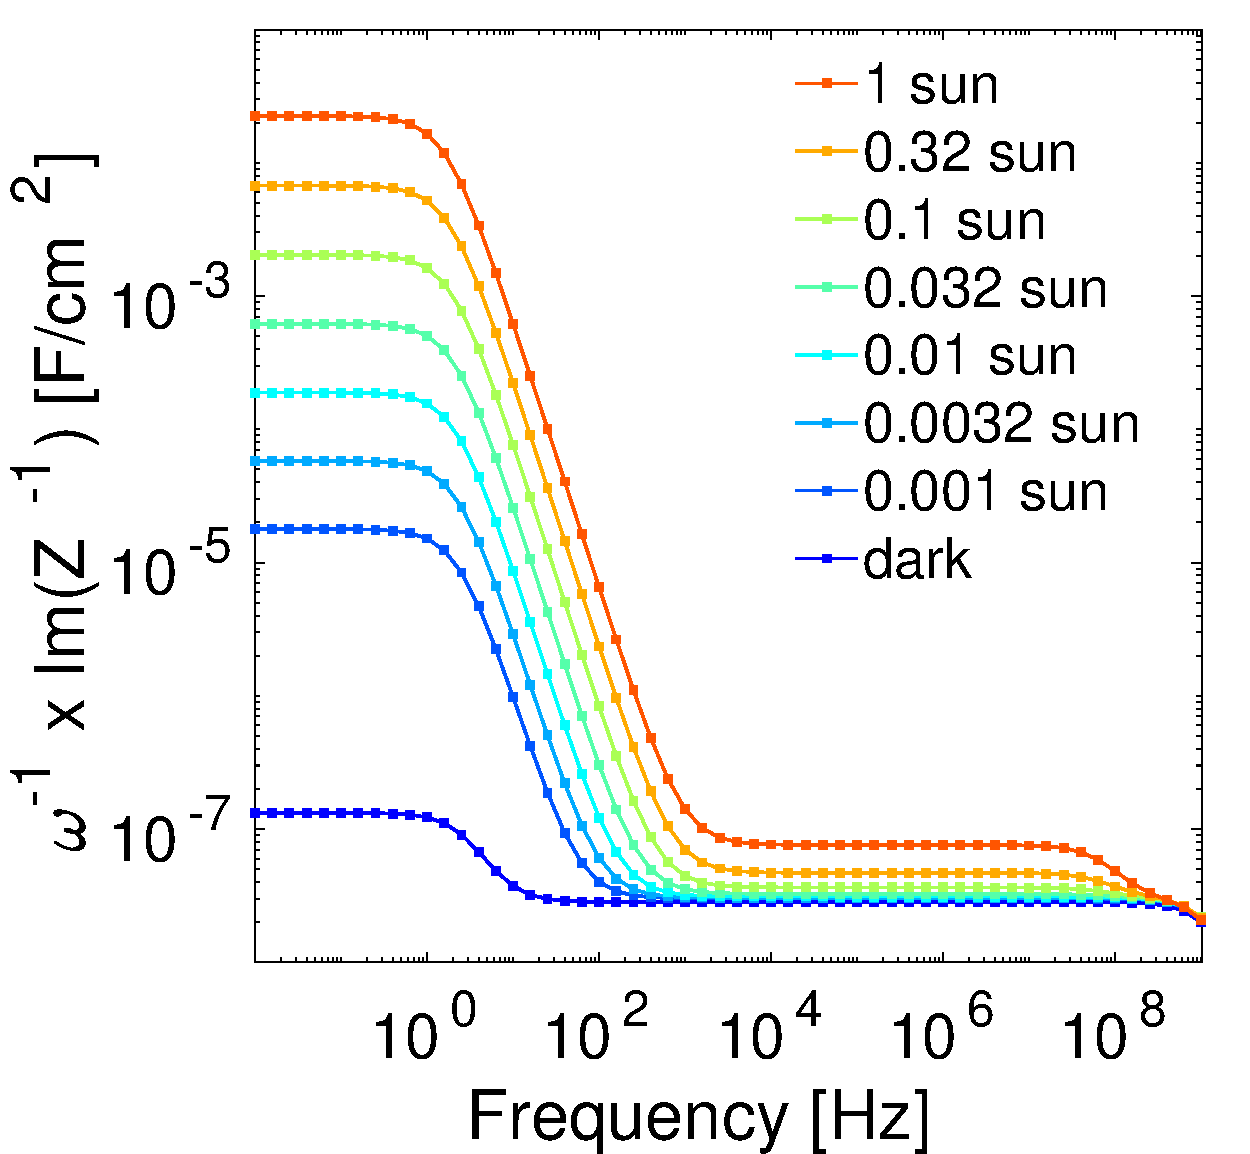
\includegraphics[width=1\textwidth]{dd_capacitance/capacitance-small.pdf}
					\subcaption{Illuminated, open circuit}\label{fig:impedance-capacitance-oc}
				\end{subfigure}
				\qquad
				\begin{subfigure}[t]{0.51\textwidth}
					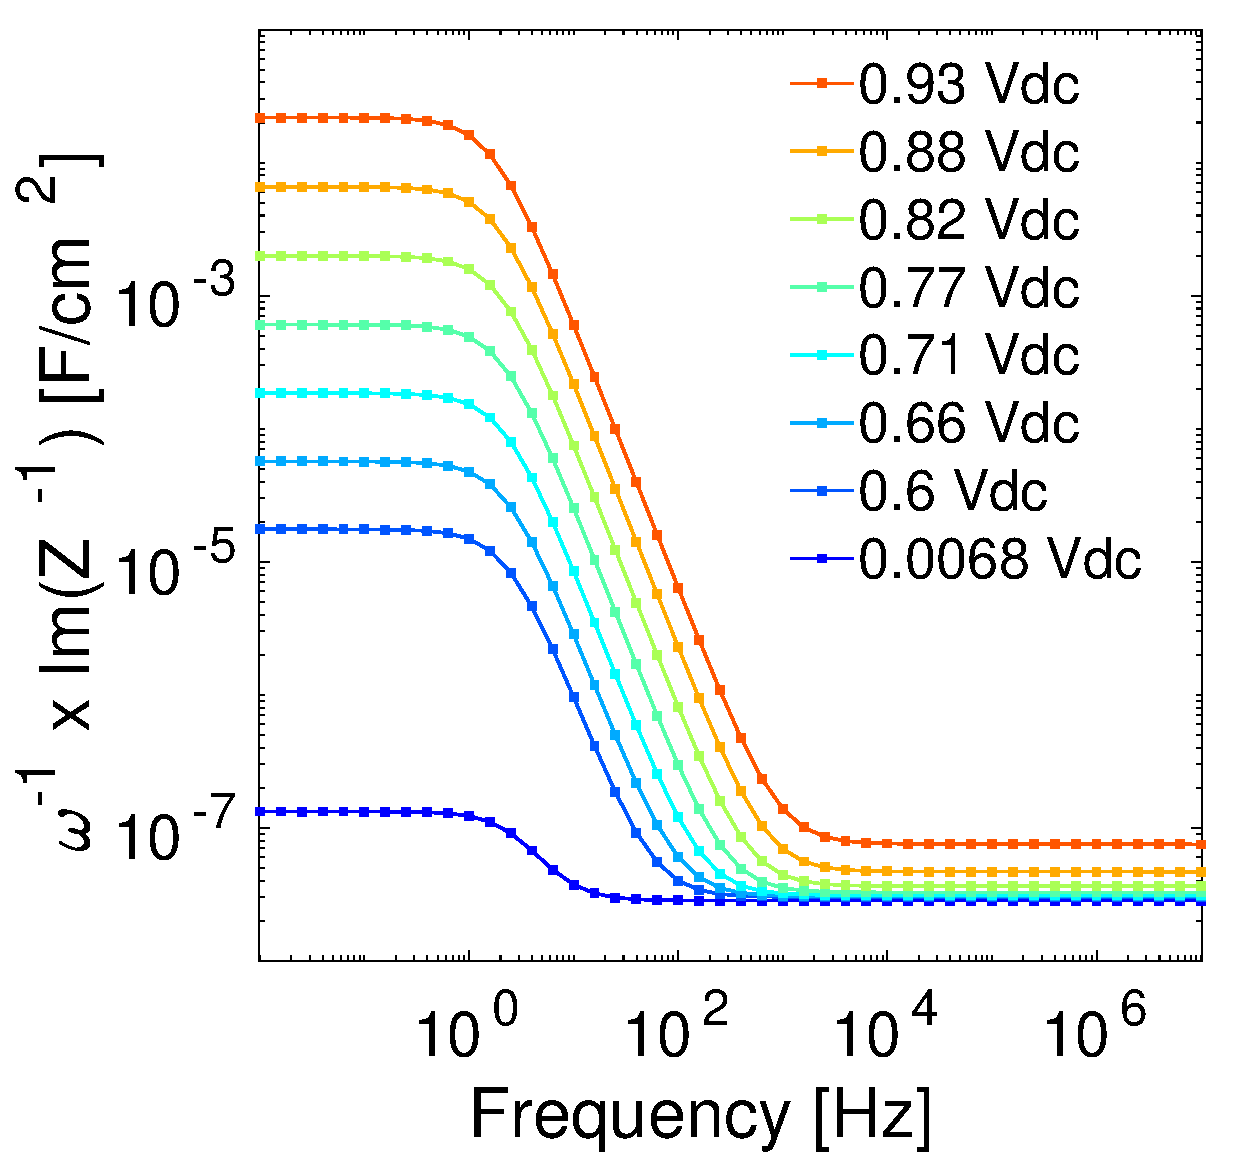
\includegraphics[width=1\textwidth]{dd_capacitance/vapp-cap-small.pdf}
					\subcaption{Dark, applied voltage}\label{fig:impedance-capacitance-vapp}
				\end{subfigure}
				\mycaption[Simulated apparent capacitance spectra of an illuminated perovskite solar cell at open circuit and dark applied voltage.]{
					In (\textbf{a}) the simulation oscillates the voltage around the \gls{voc} value induced by different light intensities at open circuit (light bias).
					In (\textbf{b}) the voltages from (\textbf{a}) are applied as constant voltage biases around which the applied voltage oscillates, in dark.
					Due to some unidentified numerical, in the dark case at \SI{0}{\V} there is a residual current.
					For eliminating this current, a voltage bias of \SI{0.0068}{V} has been applied to the dark solution in (\textbf{b}).
				}\label{fig:impedance-capacitance}
			}
		}
	\end{figure}



	\subsection{Very high frequency}
	\paragraph{Dark case}
In the simulation at frequencies above \SI{1e7}{\Hz} in dark, the voltage change is too fast for the charges to migrate from the electrodes (in our simulation, the boundaries) to the depletion\index{space charge layer} layers in the contacts.
This can be seen in \cref{fig:impedance-delta_charge-highFreq} from the presence of net charge out of the depletion\index{space charge layer} layers, at the electrodes\-/contacts interface (left and right simulation boundaries).
This happens because the oscillation period is shorter than the \gls{rctime} composed by the geometric capacitance\index{geometric capacitance} of the device (a parallel plate capacitor having the imaginary plates at the depletion\index{space charge layer} layers and the perovskite layer as dielectric) and the transport resistance in the \acr{htm} and \acr{etm} contacts.
We can see this as a non~\SI{90}{\degree} phase in the extremely high frequency region of \cref{fig:impedance-ionic-phase} and as a decrease of the apparent capacitance in \cref{fig:impedance-capacitance-oc}.
Experimentally, this is observed some times but lies close to the instrumental frequency limit (usually \SI{1e6}{\Hz}).


\begin{figure}
	\makebox[\textwidth][c]{
		\parbox{1.1\textwidth}{
			\centering
			\begin{subfigure}[t]{0.5\textwidth}
				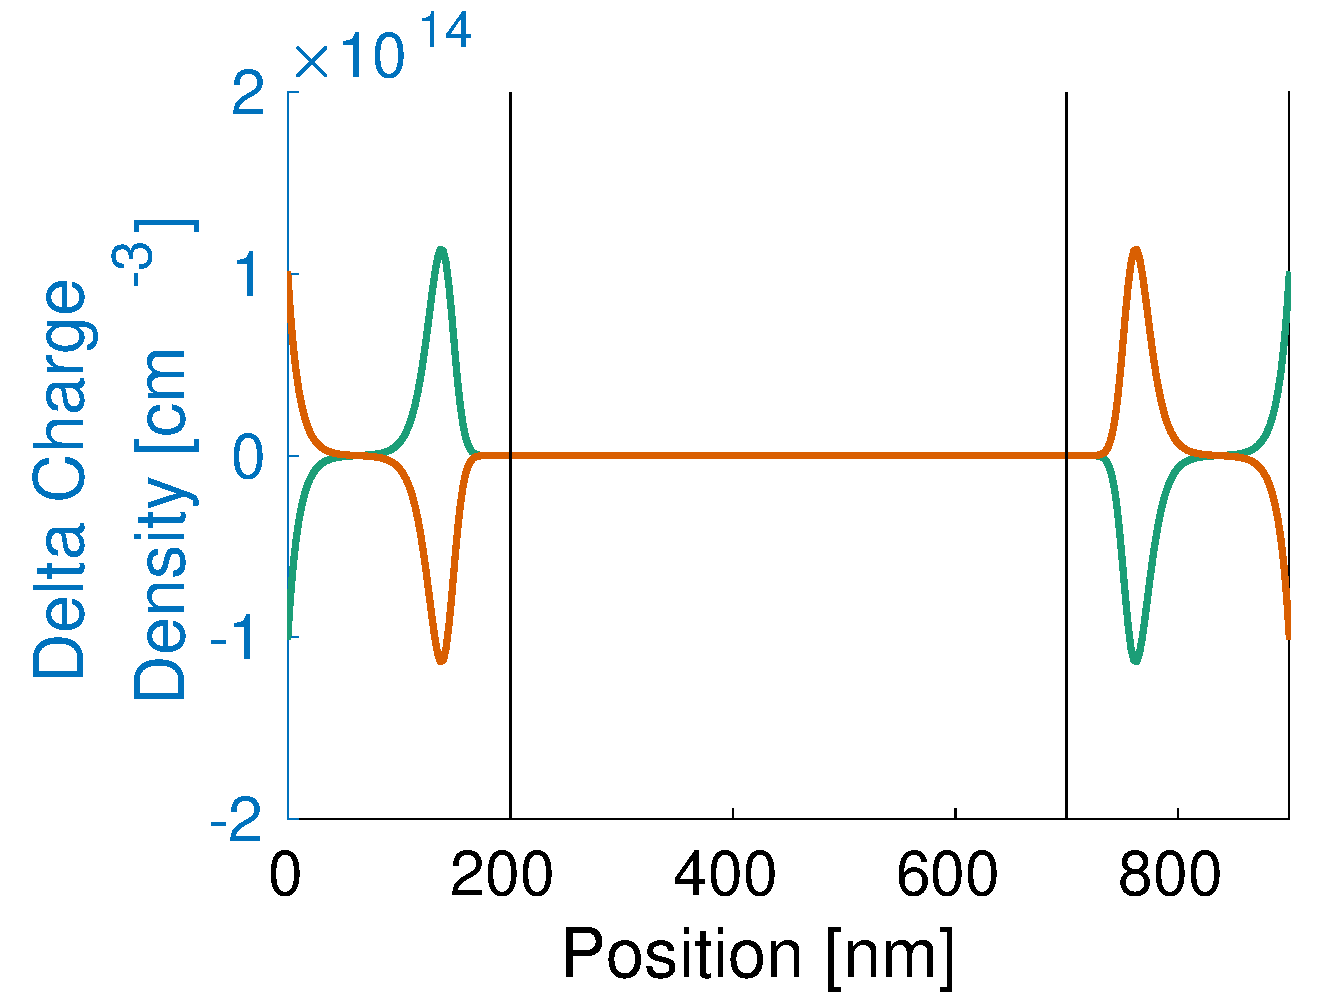
\includegraphics[width=1\textwidth]{delta_charge/delta_charge-highFreq2.pdf}
				\subcaption{Dark, high freq.}\label{fig:impedance-delta_charge-highFreq}
			\end{subfigure}
			\qquad
			\begin{subfigure}[t]{0.5\textwidth}
				\includegraphics[width=1\textwidth]{delta_charge/delta_charge-midFreq_dark2.pdf}
				\subcaption{Dark, mid freq.}\label{fig:impedance-delta_charge-midFreq_dark}
			\end{subfigure}
			\bigskip
			
			\begin{subfigure}[t]{0.5\textwidth}
				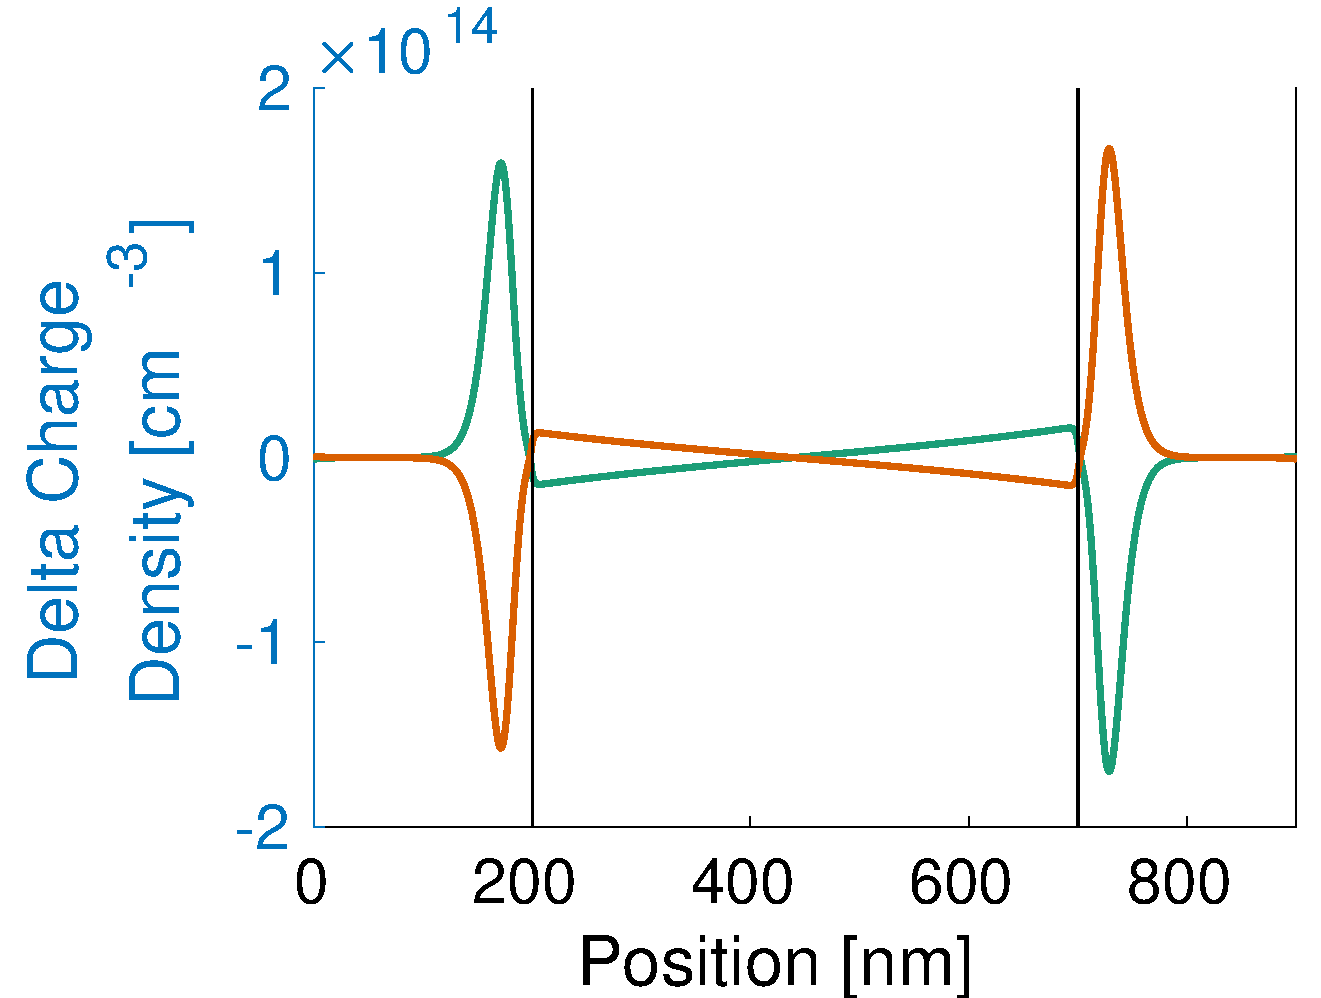
\includegraphics[width=1\textwidth]{delta_charge/delta_charge-midFreq_1sun2.pdf}
				\subcaption{1 sun, mid freq.}\label{fig:impedance-delta_charge-midFreq_1sun}
			\end{subfigure}
			\qquad
			\begin{subfigure}[t]{0.5\textwidth}
				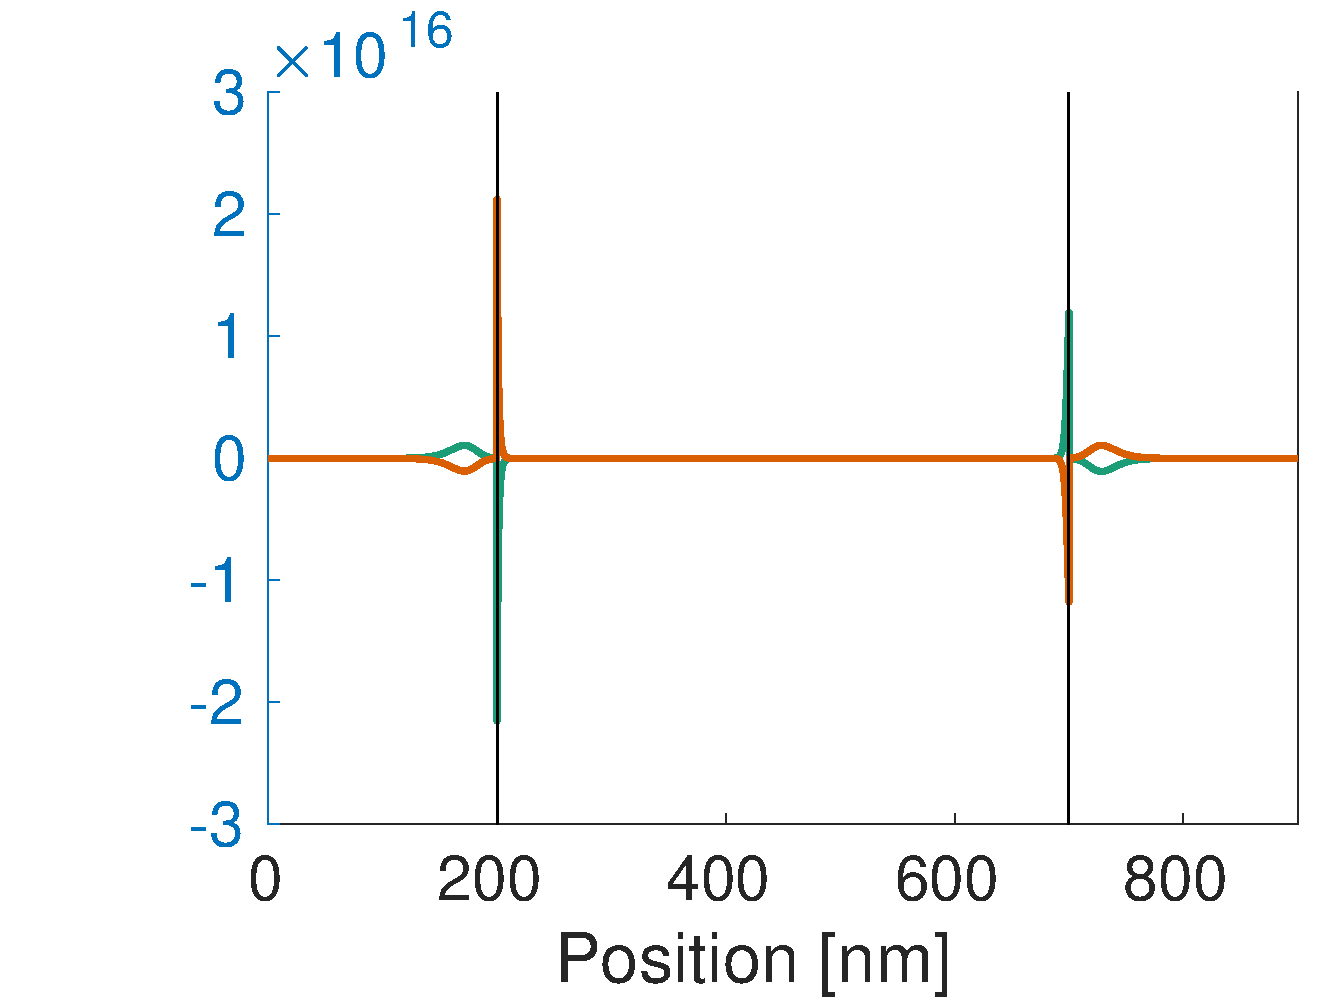
\includegraphics[width=1\textwidth]{delta_charge/delta_charge-lowFreq_1sun2.pdf}
				\subcaption{1 sun, low freq.}\label{fig:impedance-delta_charge-lowFreq_1sun}
			\end{subfigure}
			
			
			
			\mycaption[Net charge profile variation in a period of oscillating voltage at high and mid frequencies.]{
				A $p$(\SI{200}{\nm})--$i$(\SI{500}{\nm})--$n$(\SI{200}{\nm}) homojunction device is simulated.
				The space\index{space charge layer} charge layers in the device (\textsl{e.g.}\ depletion\index{space charge layer} layers in the contacts) have a net charge (unbalanced positive and negative charge densities).
				The net charge profile is obtained with $\rho(x,t) = -n(x,t) + p(x,t) + a(x,t) + n_|stat|(x)$ where $n$, $p$, and $a$ are the electrons, holes, and ions density profiles and $n_|stat|$ are the fixed charges profile, including the doping in the contacts and the fixed counter ions in the perovskite layer.
				The represented net charge variation is obtained as $\Delta \rho (x,t) = \rho(x,t) - \rho(x,0)$.
				The green line indicates the additional net charge when the oscillating voltage is at its maximum, while the orange line indicates the situation at the voltage minimum.
				In (\textbf{a}) the device is in dark and the voltage oscillates at \SI{1e9}{\Hz}; in (\textbf{b}) it is also in dark but the frequency is lower: \SI{1e6}{\Hz}; in (\textbf{c}) the frequency is also \SI{1e6}{\Hz} but the device is at \SI{1}{sun} illumination and at open circuit conditions; in (\textbf{d}) the frequency is decreased to \SI{1e-2}{\Hz} so that the ionic migration is active.
			}\label{fig:impedance-delta_charge}
		}
	}
\end{figure}

	\paragraph{Illuminated case}
	Looking at the phase in the high frequency region for \SI{1}{sun} illuminated case in \cref{fig:impedance-ionic-phase}, we can see a trend similar to the one observed for the dark case.
	One small difference is represented by a bump at \SI{1e8}{\Hz}, representing the characteristic time for the movement of the free charges in the perovskite layer.
	At frequencies lower than this point, the electrons and holes in the perovskite layer contribute to the screening of the electric field.




	\subsection{Mid frequency}
	At mid frequencies, approximatively from \SIrange{1e3}{1e7}{\Hz}, a plateau can be observed in the apparent capacitance.
	In this region, the frequency is slow enough for the contacts' depletion\index{space charge layer} layers population/depopulation and for the migration of the free carriers in the perovskite layer, as represented in \cref{fig:impedance-delta_charge-midFreq_dark}.
	
	\paragraph{Dark case}
	For the dark case, the observed capacitance of \SI{2.83e-8}{\farad\per\square\cm} is just the geometric capacitance\index{geometric capacitance} of the device.
	As explained in \cpageref{geometric_capacitance_and_voltage}, the parallel plate capacitor giving rise to this geometric capacitance\index{geometric capacitance} has an inter plate distance slightly larger than the perovskite thickness (\SI{500}{\nm}).
	The correct position of this imaginary plate is indeed in the contact's depletion\index{space charge layer} layer, more precisely where the charge concentration varies when applying the oscillating voltage.
	This distance can be estimated from the distance of the peaks in \cref{fig:impedance-delta_charge-midFreq_dark} as \SI{625}{\nm}.
	From this and from the materials' permittivity (\gls{symb:epsilonr} $20$ for all the layers, see \cref{table:impedance_parameters}) we can predict a geometric capacitance\index{geometric capacitance} of \SI{2.83e-8}{\farad\per\square\cm} which is in accordion with the value obtained from the impedance.
	
%	electric constant =
%	8.85418782 × 10-12 m-3 kg-1 s4 A2

		\paragraph{Illuminated case}
		As can be seen in \cref{fig:impedance-accumulation}, with the illumination, the apparent capacitance of the mid frequency plateau increases up to \SI{7.60e-8}{\farad\per\square\cm} at \SI{1}{sun}.
		This is caused by the large amount of free carriers in the perovskite due to the illumination (or due to the voltage bias for the dark case reported in \cref{fig:impedance-capacitance-vapp}).
		As shown in \cref{fig:impedance-delta_charge-midFreq_1sun}, the free carriers drift inside of the perovskite layer causing a dipole.
		This partially screens the electric field allowing the device to accumulate more charges and effectively increasing its capacitance.
		From the parallel plate capacitor model point of view, these charges in the dielectric layer effectively increase its permittivity.

	\begin{figure}%impedance-accumulation
				\makebox[\textwidth][c]{
		\parbox{1.1\textwidth}{
		\centering
		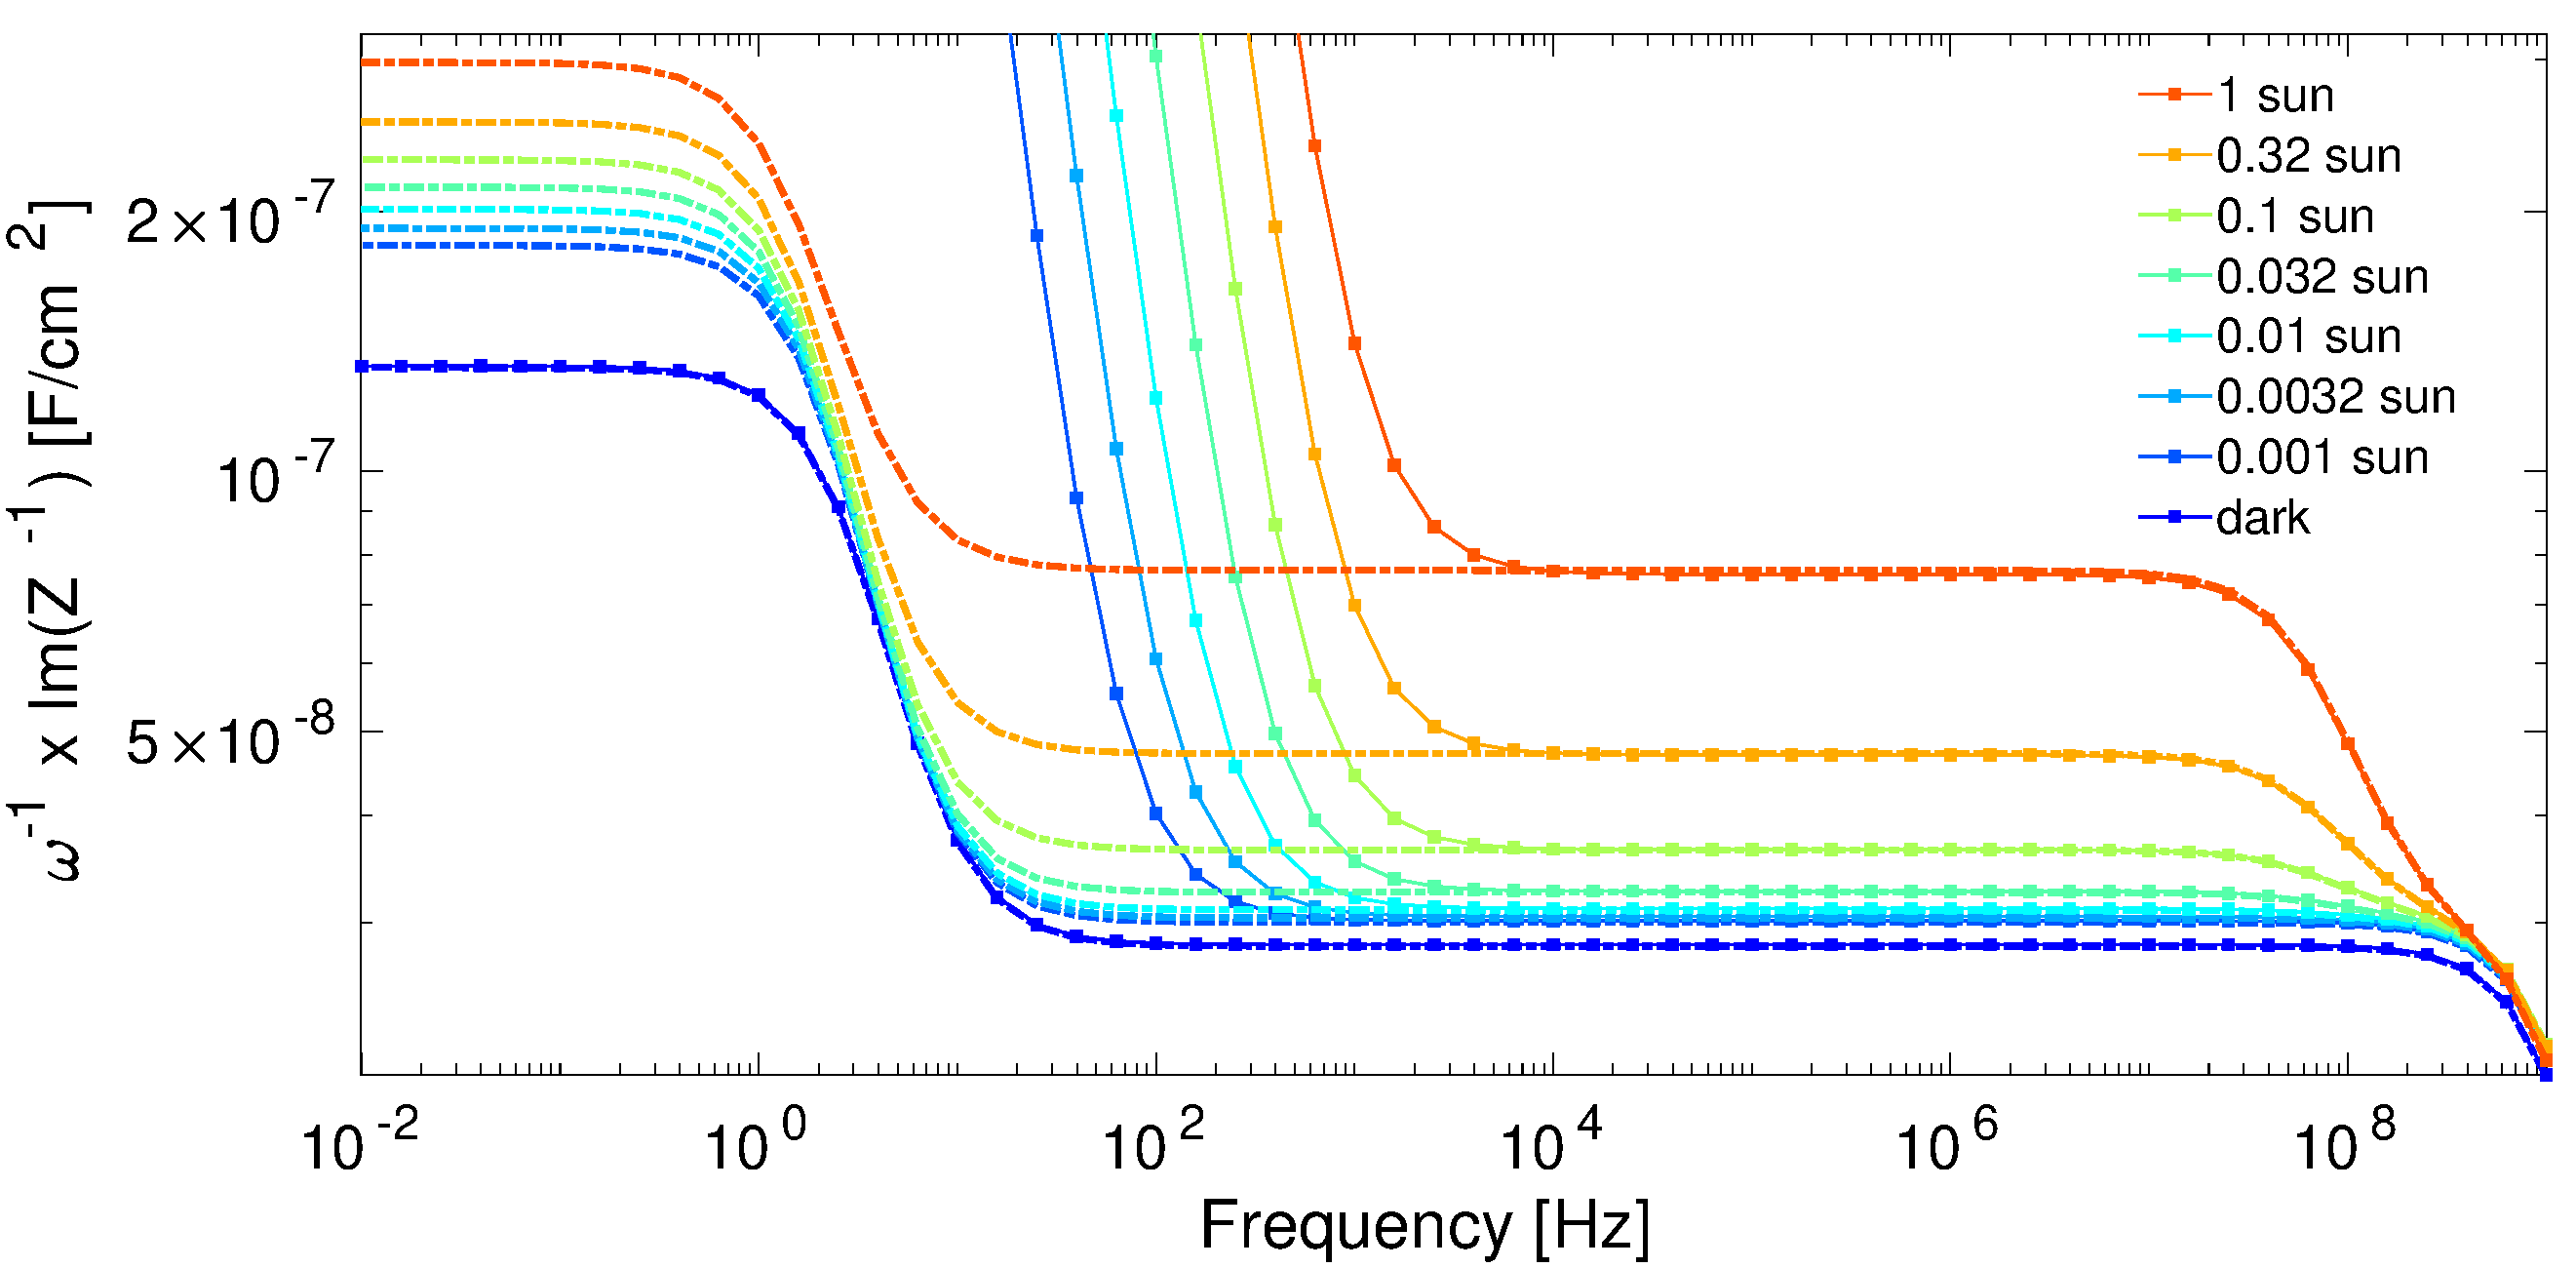
\includegraphics[width=1\textwidth]{dd_capacitance/accumulation2.pdf}
		\mycaption[Simulated accumulation capacitance spectra compared with capacitance due to charge accumulation.]{
		Solid lines with dot markers represent the apparent capacitance, dash dotted lines show the capacitance calculated from the accumulation current obtained as explained in \cpageref{impedance_accumulation}.
		For the dark case, the apparent and the accumulation capacitances correspond at any frequency.
		With illumination, the high and mid frequency regions matches while the apparent capacitance is much larger for the low frequencies.
	}\label{fig:impedance-accumulation}
}}
	\end{figure}



	\subsection{Low frequency}
	
		\begin{figure}%cap_scheme_hi_low_freq
		\makebox[\textwidth][c]{
			\parbox{1.1\textwidth}{
				\centering
				\begin{subfigure}[t]{0.51\textwidth}\centering
					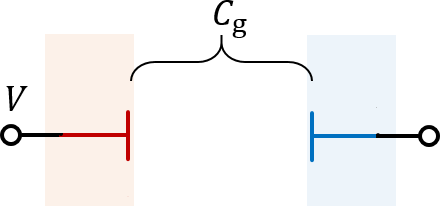
\includegraphics[width=0.7\textwidth]{cap_scheme_hi_low_freq/capacitance_no_ions.png}
					\subcaption{Capacitance at mid frequencies}\label{fig:cap_scheme_hi_freq}
				\end{subfigure}
				\qquad
				\begin{subfigure}[t]{0.51\textwidth}\centering
					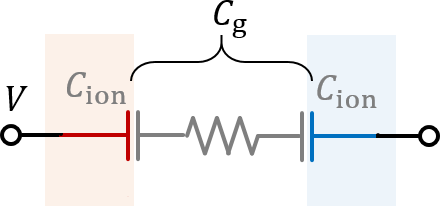
\includegraphics[width=0.7\textwidth]{cap_scheme_hi_low_freq/capacitance_with_ions.png}
					\subcaption{Capacitance at low frequencies}\label{fig:cap_scheme_low_freq}
				\end{subfigure}
				\mycaption[Capacitance representation with or without mobile ions.]{
				The area in pink indicates the \acr{htm} and the one in blue the \gls{etm}.
				In (\textbf{a}) the geometric capacitance\index{geometric capacitance} observable at mid frequencies is represented, where the charges accumulate in the contacts close to the perovskite interface.
				In (\textbf{b}) the ionic accumulation observable at low frequencies is represented as two additional capacitor plates and the ionic transport as a resistance between them.
			}\label{fig:cap_scheme_hi_low_freq}
			}
		}
	\end{figure}



	Up to now, we observed the charging and discharging of a geometric capacitance\index{geometric capacitance} with the charge accumulation in the contacts and, in some cases, in the perovskite layer.
	This is represented by the capacitor in \cref{fig:cap_scheme_hi_freq}.
	We did not consider yet the ionic motion as at mid and high frequencies it was effectively frozen: the slow ions did not have time to migrate.
	The activation of the ionic movement can be seen in the phase of ionic displacement current\index{displacement current} represented in \cref{fig:impedance-ionic-phase}.
	As we can see, once the ionic migration is active, the related current is purely capacitive (\SI{+90}{\degree}).
	This is expected as the ionic species can just accumulate or deplete at the interfaces of the perovskite layer with the contacts (simulations where ions could penetrate in the contacts have been performed but will not be reported in this thesis) screening the electric field, like in the capacitor represented in \cref{fig:cap_scheme_low_freq}.
	



	\paragraph{Dark case}\label{impedance_lowf_dark}
	Experimentally, a feature at frequencies \SI{< 100}{\Hz} is often observed in impedance of perovskite solar cells in dark \cite{Pockett2015,Juarez-Perez2014,Kim2015c,Guerrero2016,Zarazua2016}.
	This feature has been interpreted as a ionic influence on the dark capacitance by \authoryear{Yang2015e}.
	Indeed, calculating an apparent capacitance value from the ionic displacement current\index{displacement current} (see \cpageref{displacement_current_ionic,intro_displacement_current}) we can see that it matches the apparent capacitance value in dark, reported in \cref{fig:impedance-ionic-capacitance}.
	Differently from the geometric capacitance\index{geometric capacitance} observed at mid frequencies, this low frequency capacitance value is independent from the perovskite layer thickness, as it relates just to the interfacial region, neglecting any contribution from the perovskite bulk.
	In case the ionic capacitance is smaller than the geometric capacitance\index{geometric capacitance} (\textsl{e.g.}\ if the ionic concentration is not high enough for screening the electric field or with a very thin device), no bump can be seen and just the geometric capacitance\index{geometric capacitance} is observed at low frequency.
	As a concept, this ionic capacitance is similar to the "junction capacitance" or "transition capacitance" of the interface between a $p$-type and a $n$-type material but in this case one of the materials has ions rather than electrons or holes.


\begin{figure}%impedance-ionic
	\makebox[\textwidth][c]{
		\parbox{1.1\textwidth}{
			\centering
			\begin{subfigure}[t]{1.1\textwidth}\centering
				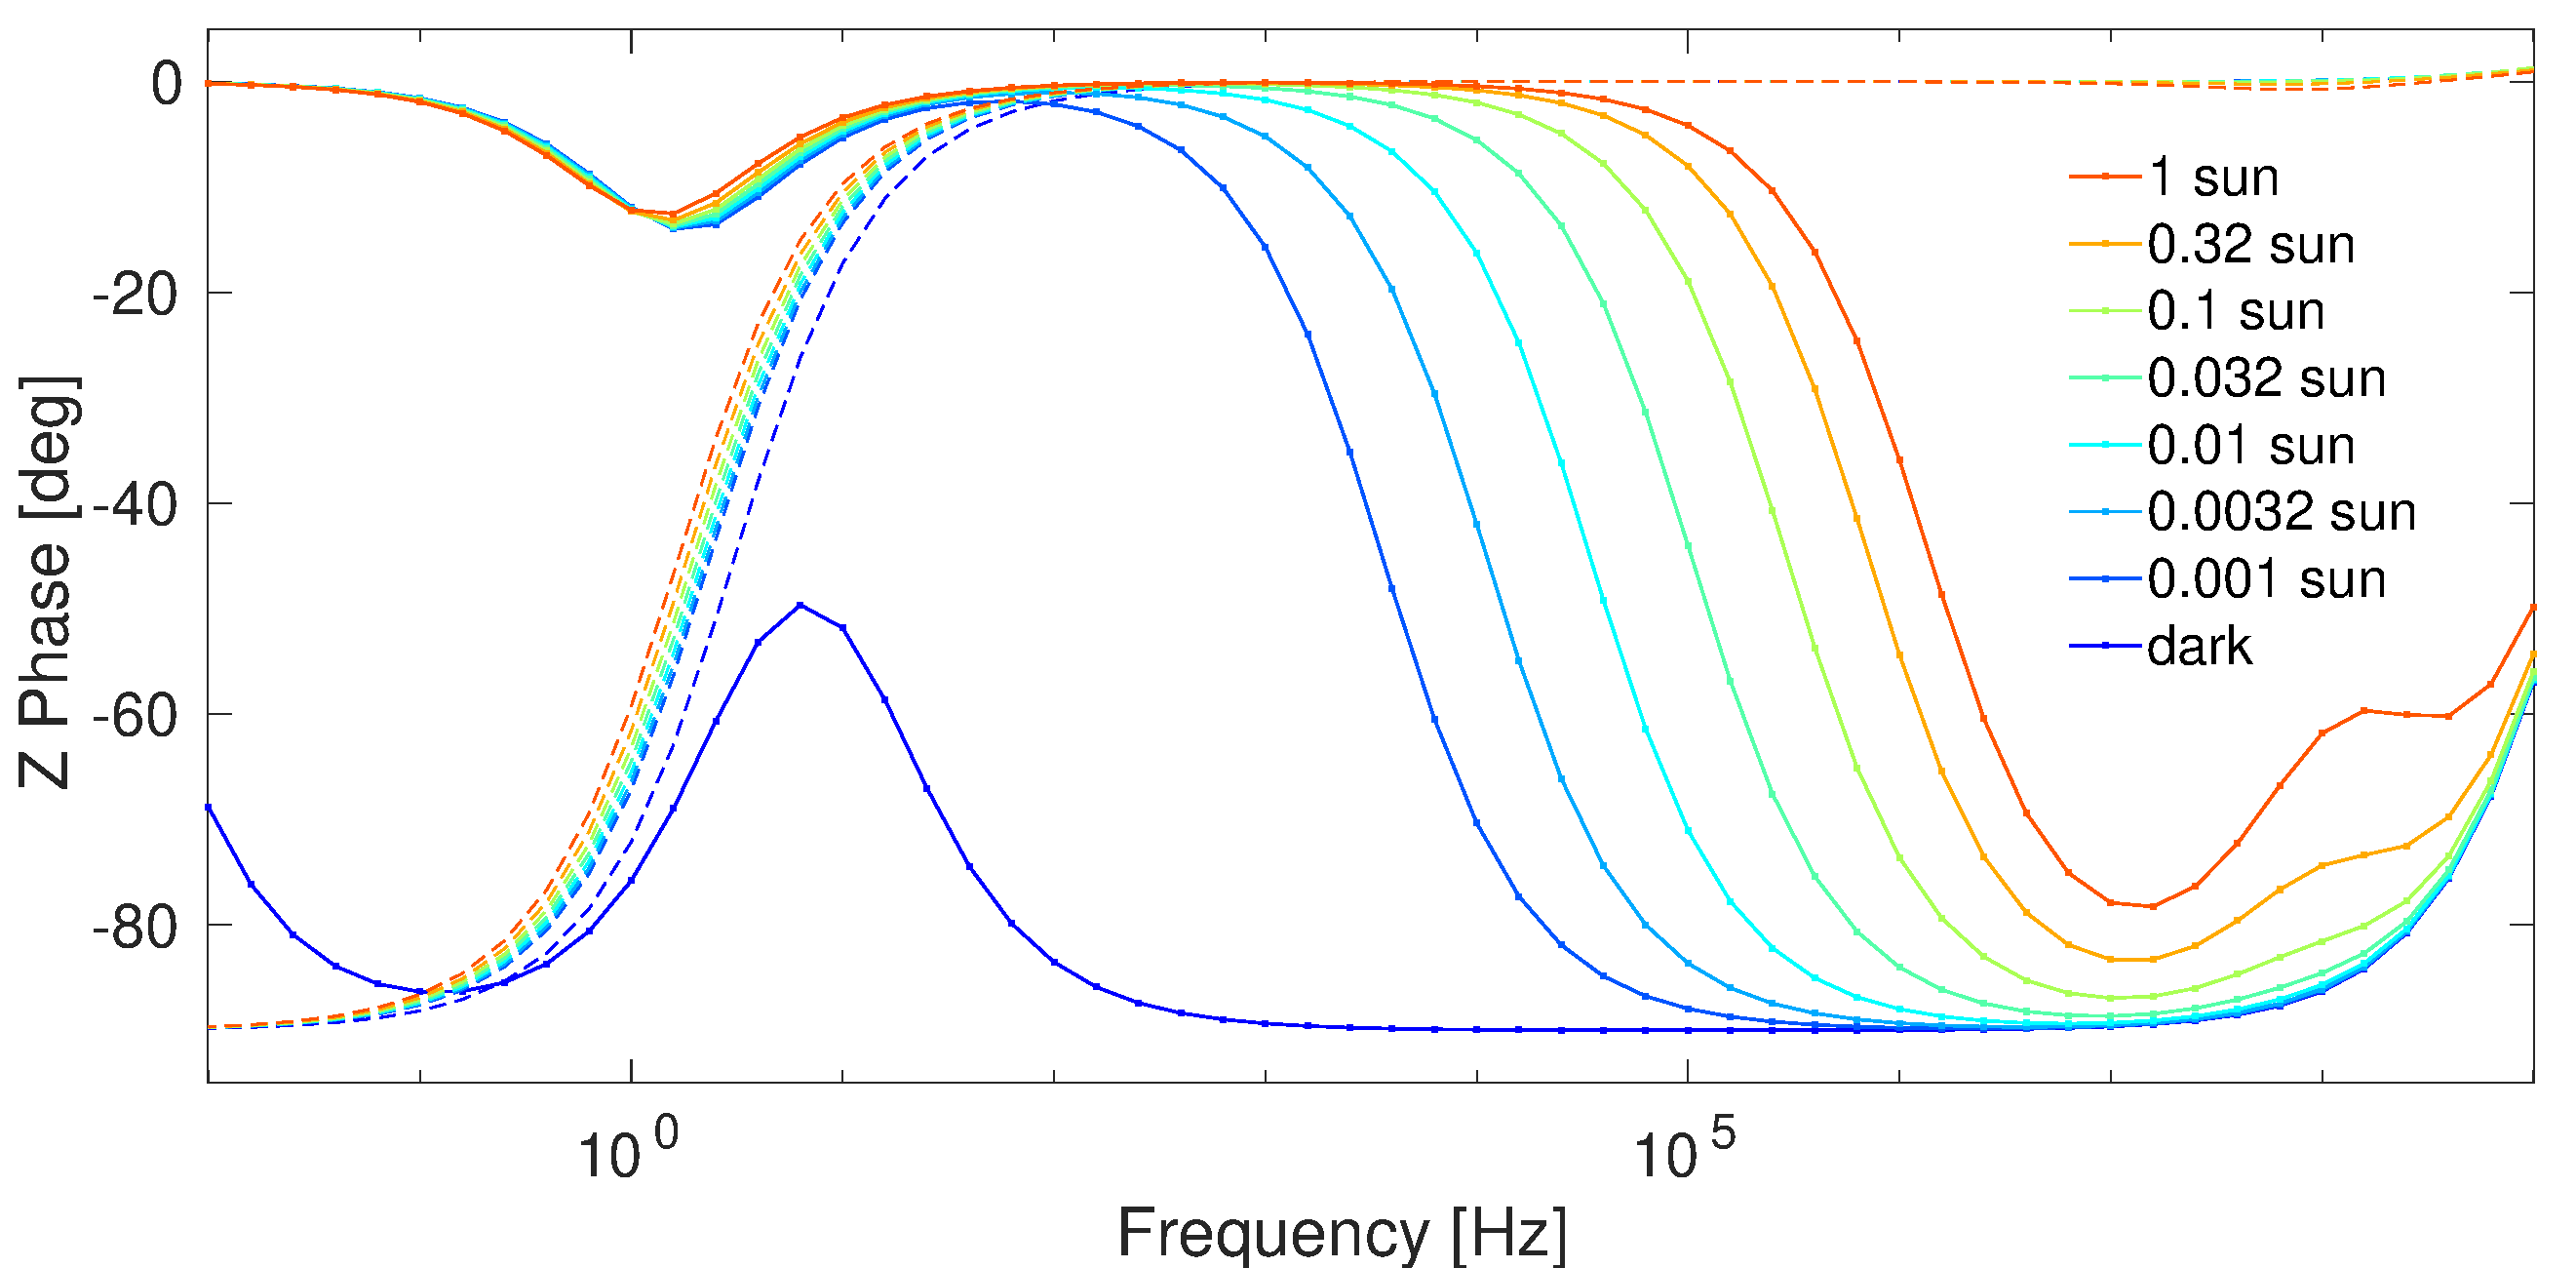
\includegraphics[width=0.9\textwidth]{dd_phase/phase.pdf}
				\subcaption{Ionic displacement current\index{displacement current} phase}\label{fig:impedance-ionic-phase}
			\end{subfigure}
			\bigskip
			
			\begin{subfigure}[t]{1.1\textwidth}\centering
				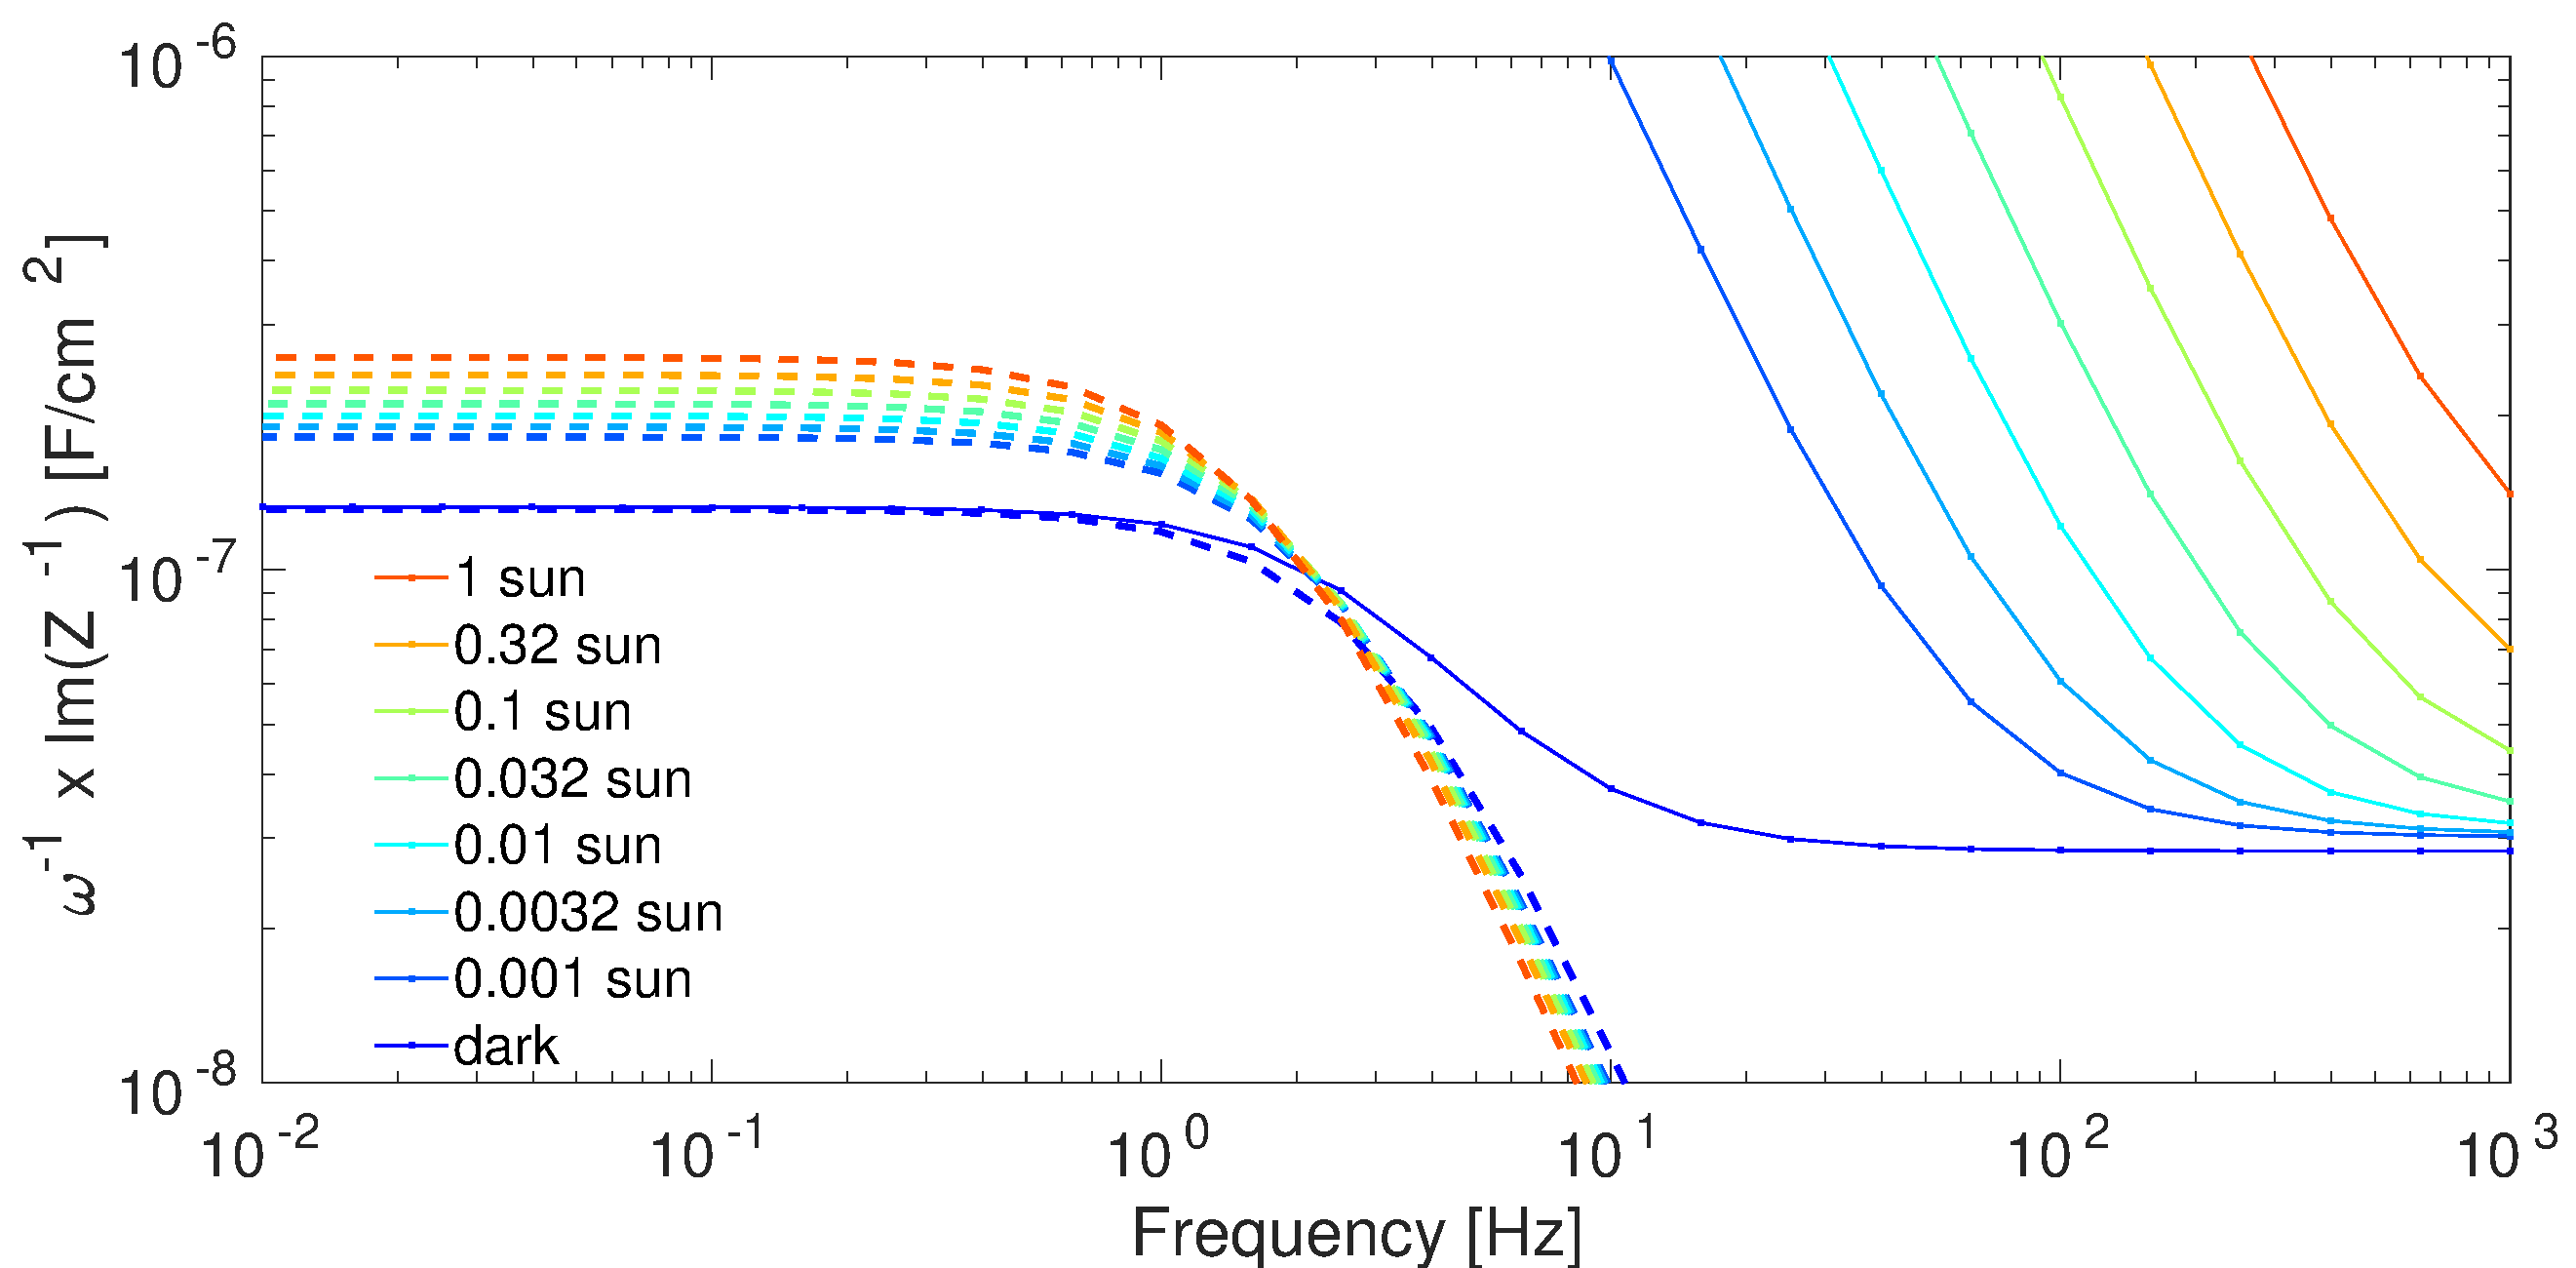
\includegraphics[width=0.9\textwidth]{dd_capacitance/ionic.pdf}
				\subcaption{Ionic displacement current\index{displacement current} capacitance}\label{fig:impedance-ionic-capacitance}
			\end{subfigure}
			
			\mycaption[Simulated apparent capacitance and phase spectra compared with capacitance due to ionic migration.]{
				In (\textbf{a}) the phase of the impedance (solid lines, it is the same as the oscillating current phase but with the opposite sign) is plotted and compared with the phase of the ionic current (dashed lines, changed of sign for easing the comparison).
				In (\textbf{b}) the apparent capacitance spectra (solid lines) is compared with the capacitance calculated from the out\hyp{}of\hyp{}phase ionic current (dashed lines).
			}\label{fig:impedance-ionic}
		}
	}
\end{figure}



	\paragraph{Illuminated case -- Observation}
Under illumination or dark but with constant voltage bias, the mentioned low frequency feature has been observed to become giant\index{giant capacitance}, increasing linearly with the light intensity \cite{Juarez-Perez2014,Kim2015c,Zarazua2016,Zarazua2016a,Almora2018}.
The available explanations in literature relied on a very large accumulation of free charges at the interfaces caused by the ionic accumulation in the same zone.
We were able to reproduce this behaviour without observing the expected huge charge concentration.
The origin of our observation was the influence of the ionic accumulation on the interface energetics and, specifically, on the recombination barrier.


	\paragraph{Illuminated case -- Not just accumulation}
	As can be seen in the low frequency region of \cref{fig:impedance-accumulation}, just the dark case can be explained by the accumulation capacitance resulting from the charges actually being stored in the device.
	When the an illumination or a voltage bias are applied, the accumulation capacitance increases by less than one order of magnitude, so the giant\index{giant capacitance} capacitance experimentally observed is not due to an accumulation of charges.
	This variation can be understood considering the different thickness of the depletion\index{space charge layer} layers in the contacts depending on the voltage bias, as explained in \cpageref{geometric_capacitance_and_voltage} for the voltage dependent geometric capacitance\index{geometric capacitance}.
	Considering the parallel plates capacitor model, at low frequency we are observing one plate in the contact's depletion\index{space charge layer} layer and the other contact in the perovskite at the interface, where we assume the ionic accumulation layer to be thin thanks to their abundance.
	Comparing \cref{fig:impedance-delta_charge-midFreq_dark} with \cref{fig:impedance-delta_charge-midFreq_1sun} we can see how the different thickness of the space\index{space charge layer} charge layers with different bias voltages (or dark \textsl{versus} \SI{1}{sun}) implies that the charge variation happens at different distances from the materials' interface.
	This implies a higher accumulation capacitance at \SI{1}{sun}, which means more charge getting accumulated and depleted in the space\index{space charge layer} charges during the voltage oscillation.
	
	
	\begin{figure}%diode_transistor
		\makebox[\textwidth][c]{
			\parbox{1.1\textwidth}{
				\centering
				\begin{subfigure}[t]{0.51\textwidth}
					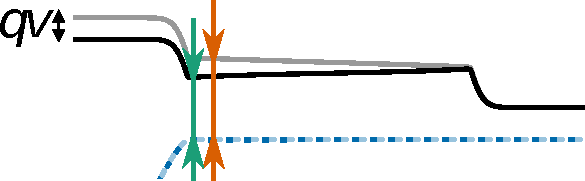
\includegraphics[width=1\textwidth]{diode_transistor/CB-high_freq-arrows.pdf}
					\subcaption{Conduction band at high frequency}\label{fig:diode_transistor-band_diagram_hifreq}
				\end{subfigure}
				\qquad
				\begin{subfigure}[t]{0.51\textwidth}
					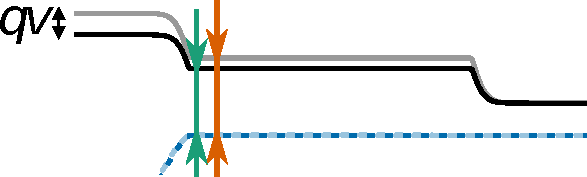
\includegraphics[width=1\textwidth]{diode_transistor/CB-low_freq-arrows.pdf}
					\subcaption{Conduction band at low frequency}\label{fig:diode_transistor-band_diagram_lowfreq}
				\end{subfigure}
				\bigskip
				
				\begin{subfigure}[t]{0.51\textwidth}\centering
					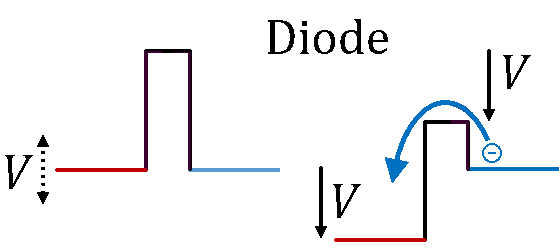
\includegraphics[width=0.7\textwidth]{diode_transistor/diode_scheme.png}
					\subcaption{Energy barrier in a diode}\label{fig:diode_transistor-diode_scheme}
				\end{subfigure}
				\qquad
				\begin{subfigure}[t]{0.51\textwidth}\centering
					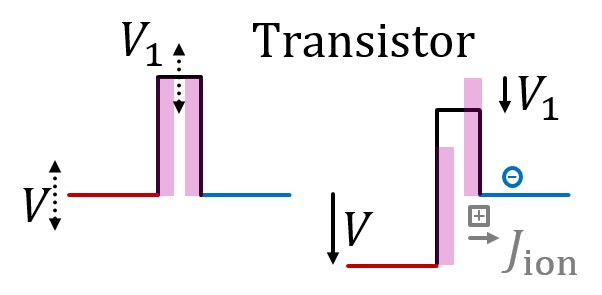
\includegraphics[width=0.8\textwidth]{diode_transistor/transistor_scheme.png}
					\subcaption{Energy barrier in a transistor}\label{fig:diode_transistor-transistor_scheme}
				\end{subfigure}
				\bigskip
				
				\begin{subfigure}[t]{0.51\textwidth}
					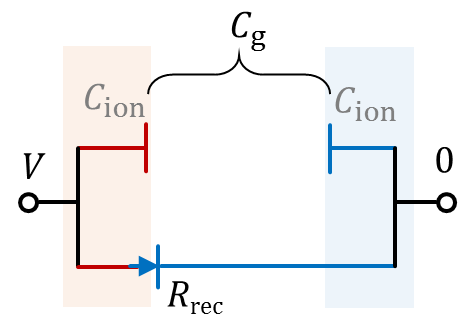
\includegraphics[width=1\textwidth]{diode_transistor/diode_noions.png}
					\subcaption{Equivalent circuit with diode}\label{fig:diode_transistor-diode}
				\end{subfigure}
				\qquad
				\begin{subfigure}[t]{0.51\textwidth}
					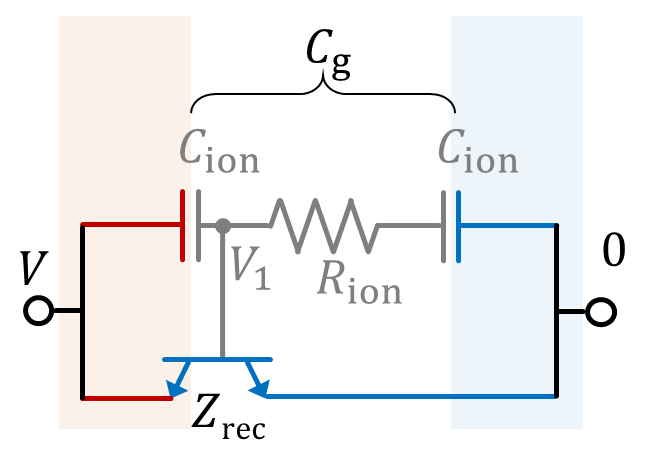
\includegraphics[width=0.9\textwidth]{diode_transistor/transistor.png}
					\subcaption{Equivalent circuit with transistor}\label{fig:diode_transistor-transistor}
				\end{subfigure}
				\mycaption[Band diagram, energy barriers, and circuit representation of a diode or a transistor.]{
					The conduction band (solid lines) and electron quasi\hyp{}Fermi level (dashed lines) of a \acr{htm} (left) perovskite (centre) \acr{etm} (right) solar cell is represented as varied by an oscillating voltage at mid and high frequencies in (\textbf{a}) and at low frequencies in (\textbf{b}).
					The electrons recombination barrier is indicated in green for the minimum applied voltage and orange for the maximum one.
					In (\textbf{c}) the energy barrier (black line) in a diode with applied voltage $V$ is represented.
					In (\textbf{d}) the energy barrier in a transistor is represented, with contributions from the applied voltage $V$ and an external voltage $V_1$.
					Pink rectangles indicating the barrier for the non-biassed case are added as graphical reference.
					In (\textbf{e}) a classical circuit including the geometric capacitance\index{geometric capacitance} and the Schottky junction diode is represented, it matches the perovskite solar cells behaviour at mid and high frequencies.
					In (\textbf{f}) the ionic accumulation is represented as a ionic capacitor, ionic transport as a resistance, the influence of ionic accumulation on the interfacial diode is made explicit by the inclusion of a transistor where the potential in ionic branch acts as a gate.
				}\label{fig:diode_transistor}
			}
		}
	\end{figure}
	
	
	
		\paragraph{Illuminated case -- Not just ions}
	Looking at the low frequency region of \cref{fig:impedance-ionic-capacitance}, we can see how the ionic capacitance (so the amount of displaced ions) increases with the illumination or applied voltage.
	This is just due to the wider charge density variation in the contacts, as observed in the previous paragraph.
	Indeed the increase in ionic capacitance is more or less similar to the increase in accumulation capacitance, and neither this can itself explain a giant\index{giant capacitance} capacitance.

	\paragraph{Illuminated case -- Recombination barriers without ions}
Let me go back to a "normal" solar cell with no mobile ions.
In most of the solar cells and in the ions free systems, the recombination flux (the current of particles entering the device and annihilating either \textsl{via} radiative or trap mediated recombination) is expected to vary coherently with the applied voltage.
In these cases, the device interfaces are usually considered like a $p$-$n$ junction diode, where the energy barrier just depends on the voltage across it as represented in \cref{fig:diode_transistor-diode_scheme}.
When we simulate a perovskite solar cell at mid and high frequency we are in this same situation:
the applied voltage is experienced as an electric field in the intrinsic layer and the recombination barrier represented in \cref{fig:diode_transistor-band_diagram_hifreq} vary by the same amount and in the same moment as the applied voltage.
So the recombination current (which depends on the recombination energy barrier) varies in\hyp{}phase with the oscillating voltage.
The equivalent electrical circuit for this regime is represented in \cref{fig:diode_transistor-diode}.


	\paragraph{Illuminated case -- Recombination barriers with ions}
When we simulate in the low frequency regime, the ions accumulate and deplete close to the interface in a capacitive manner, as described in the previous paragraph and represented in \cref{fig:impedance-delta_charge-lowFreq_1sun}.
In our simulation, the ionic concentration was enough to screen the electric field inside the perovskite layer within a few tens of nanometres from the material's interfaces.
In the low frequency, the ions have time for continuously screening the field induced by the varying voltage, as represented in \cref{fig:diode_transistor-band_diagram_lowfreq}.
Contrariwise to what happened at mid and high frequencies in \cref{fig:diode_transistor-band_diagram_hifreq}, we can see how at low frequency the variation of the recombination energy barrier is not just the applied voltage.
The electrostatic contribution by the high concentration of ionic charge also contributes to this barrier.
Checking the energy barrier in a transistor, as represented in \cref{fig:diode_transistor-transistor_scheme}, we can see how this circuit element can include the contribution of two different potentials: the applied voltage $V$ and the ionic electrostatic potential $V_1$.
In the equivalent electrical circuit, we can include the ionic capacitance as in \cref{fig:cap_scheme_low_freq} and replace the interfacial diode with a transistor having the ionic potential as the gating potential, as represented in \cref{fig:diode_transistor-transistor}.
So, now we know that the recombination current will depend both on the applied voltage and on the capacitive ionic current.
The latter contribution, being capacitive, happens \SI{90}{\degree} out\hyp{}of\hyp{}phase with regards to the oscillating applied voltage.
This key point means that the, otherwise in-phase, recombination current gains an out\hyp{}of\hyp{}phase component due to the ionic motion.
This out\hyp{}of\hyp{}phase current, as pointed out in \cref{eq:impedance_cap_1}, contributes to the apparent capacitance.
Indeed, if we use the recombination current, calculated as described in \cpageref{impedance_recombination}, for calculating an impedance and the relative apparent capacitance, we can see that this matches perfectly the simulated apparent capacitance, as reported in \cref{fig:impedance-recombination}.
This low frequency feature accounts for the arch on the right of the Nyquist plot represented in \cref{fig:impedance-nyquist}.


\begin{figure}%impedance-recombination_nyquist
	\makebox[\textwidth][c]{
		\parbox{1.1\textwidth}{
			\centering
			\begin{subfigure}[t]{1.1\textwidth}\centering
				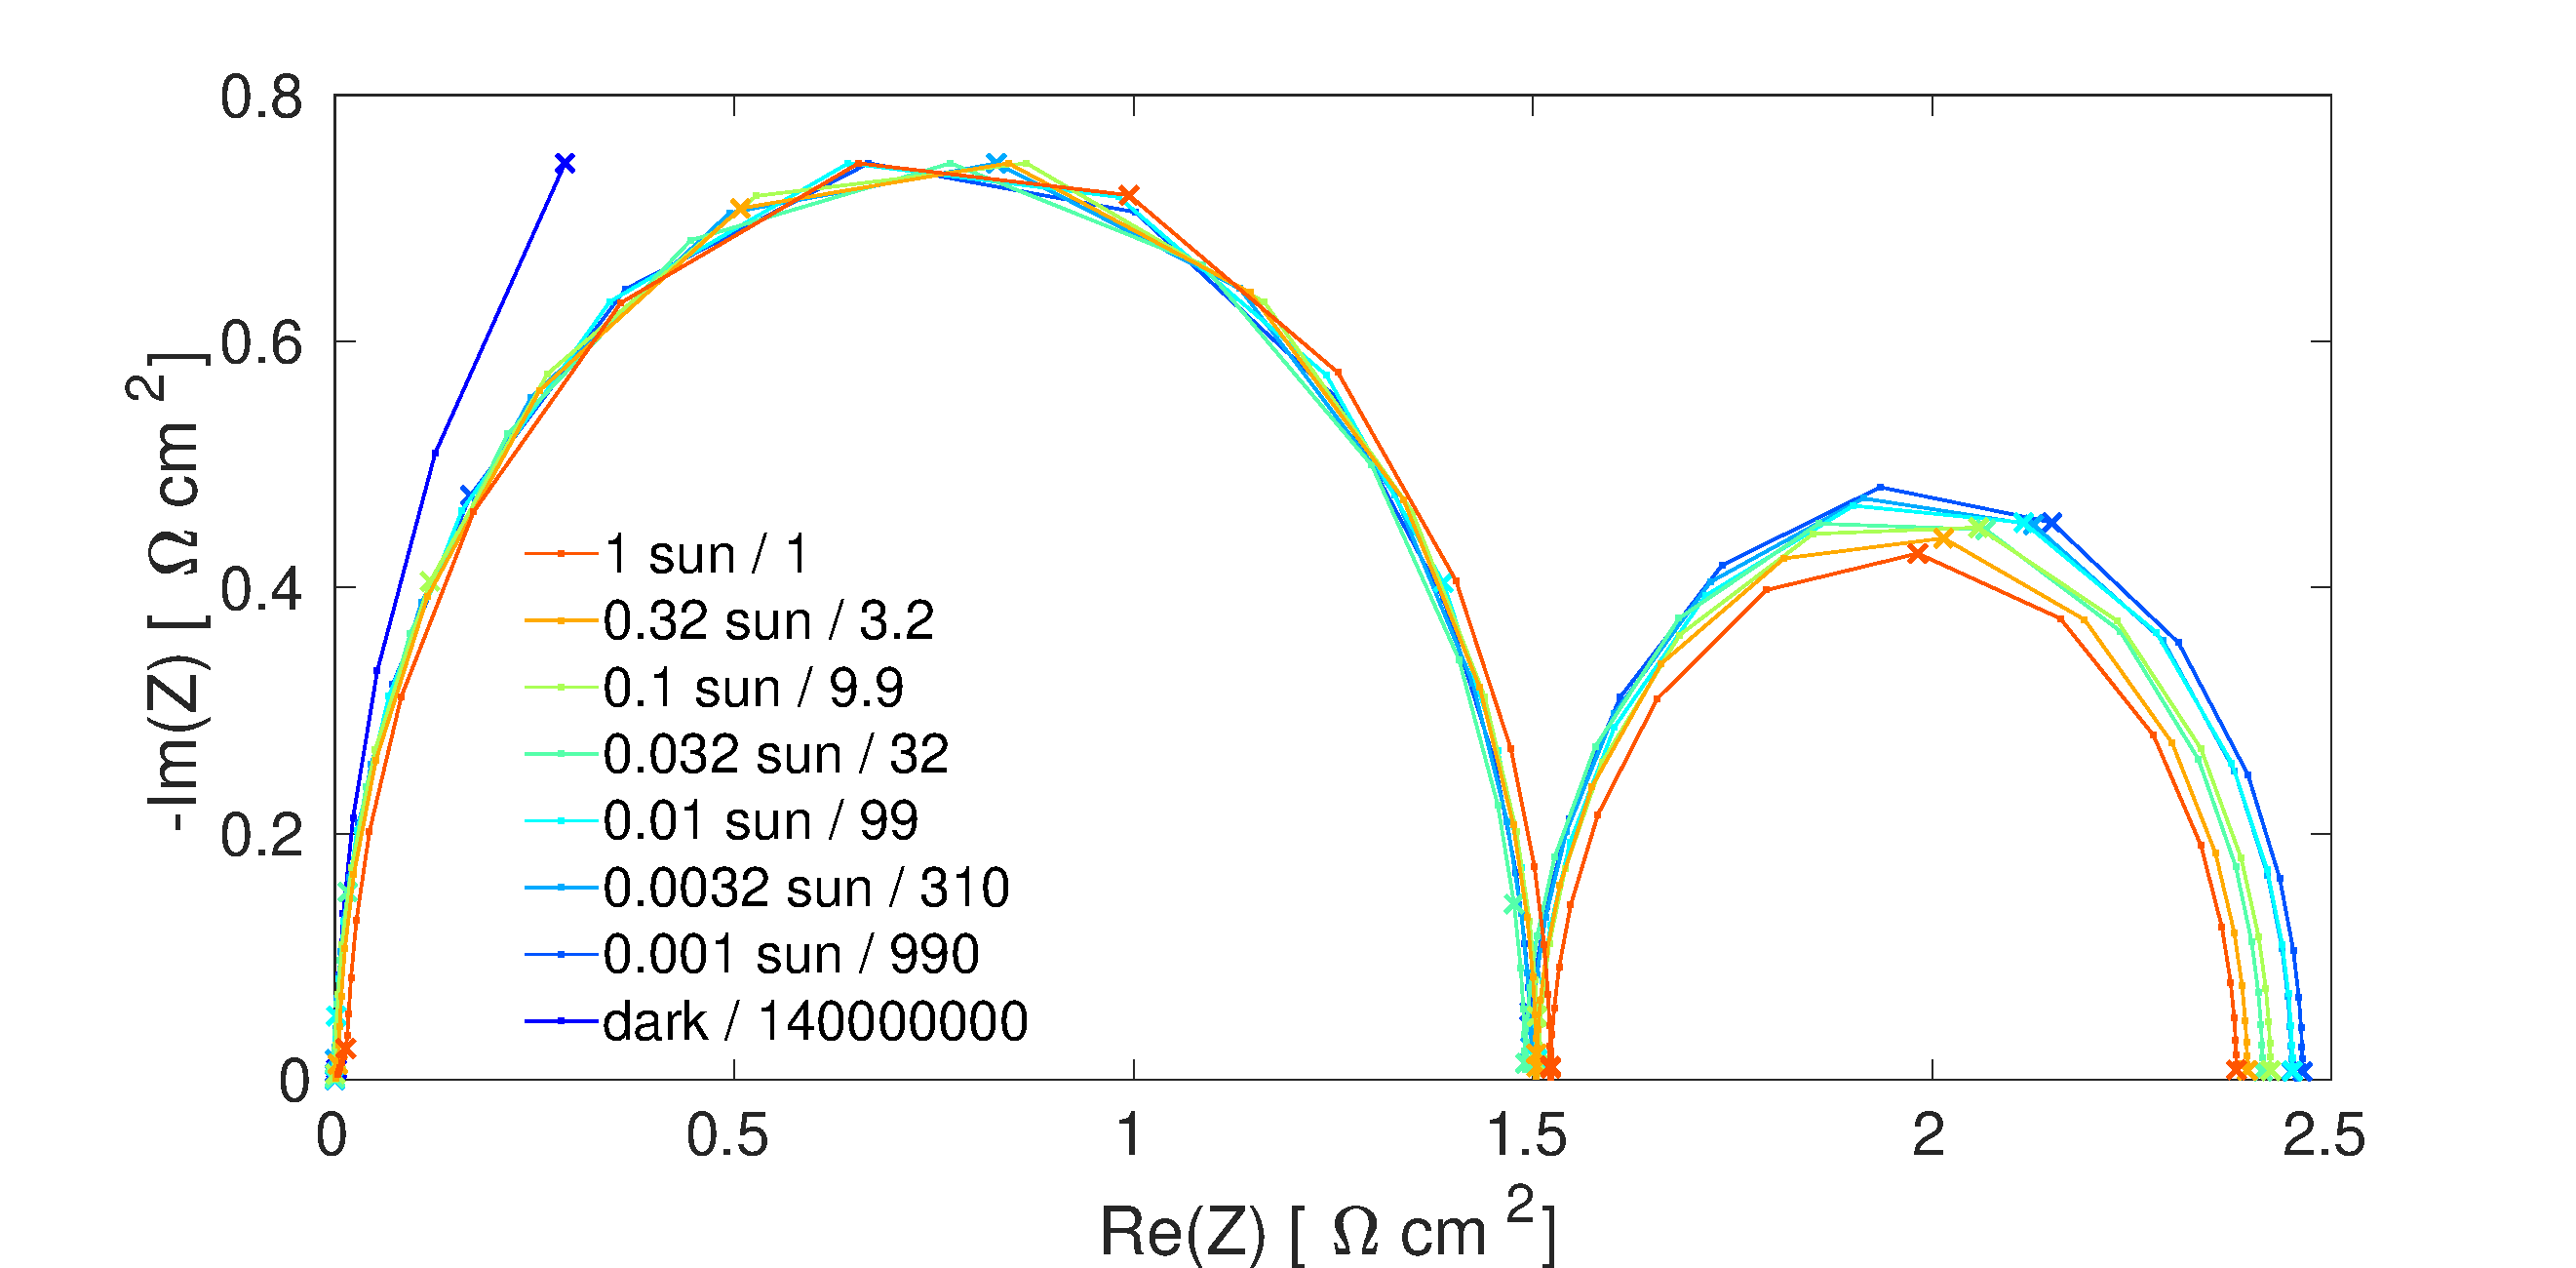
\includegraphics[width=0.9\textwidth]{dd_nyquist/nyquist_normalised.pdf}
				\subcaption{Nyquist plot}\label{fig:impedance-nyquist}
			\end{subfigure}
			\bigskip
			
			\begin{subfigure}[t]{1.1\textwidth}\centering
				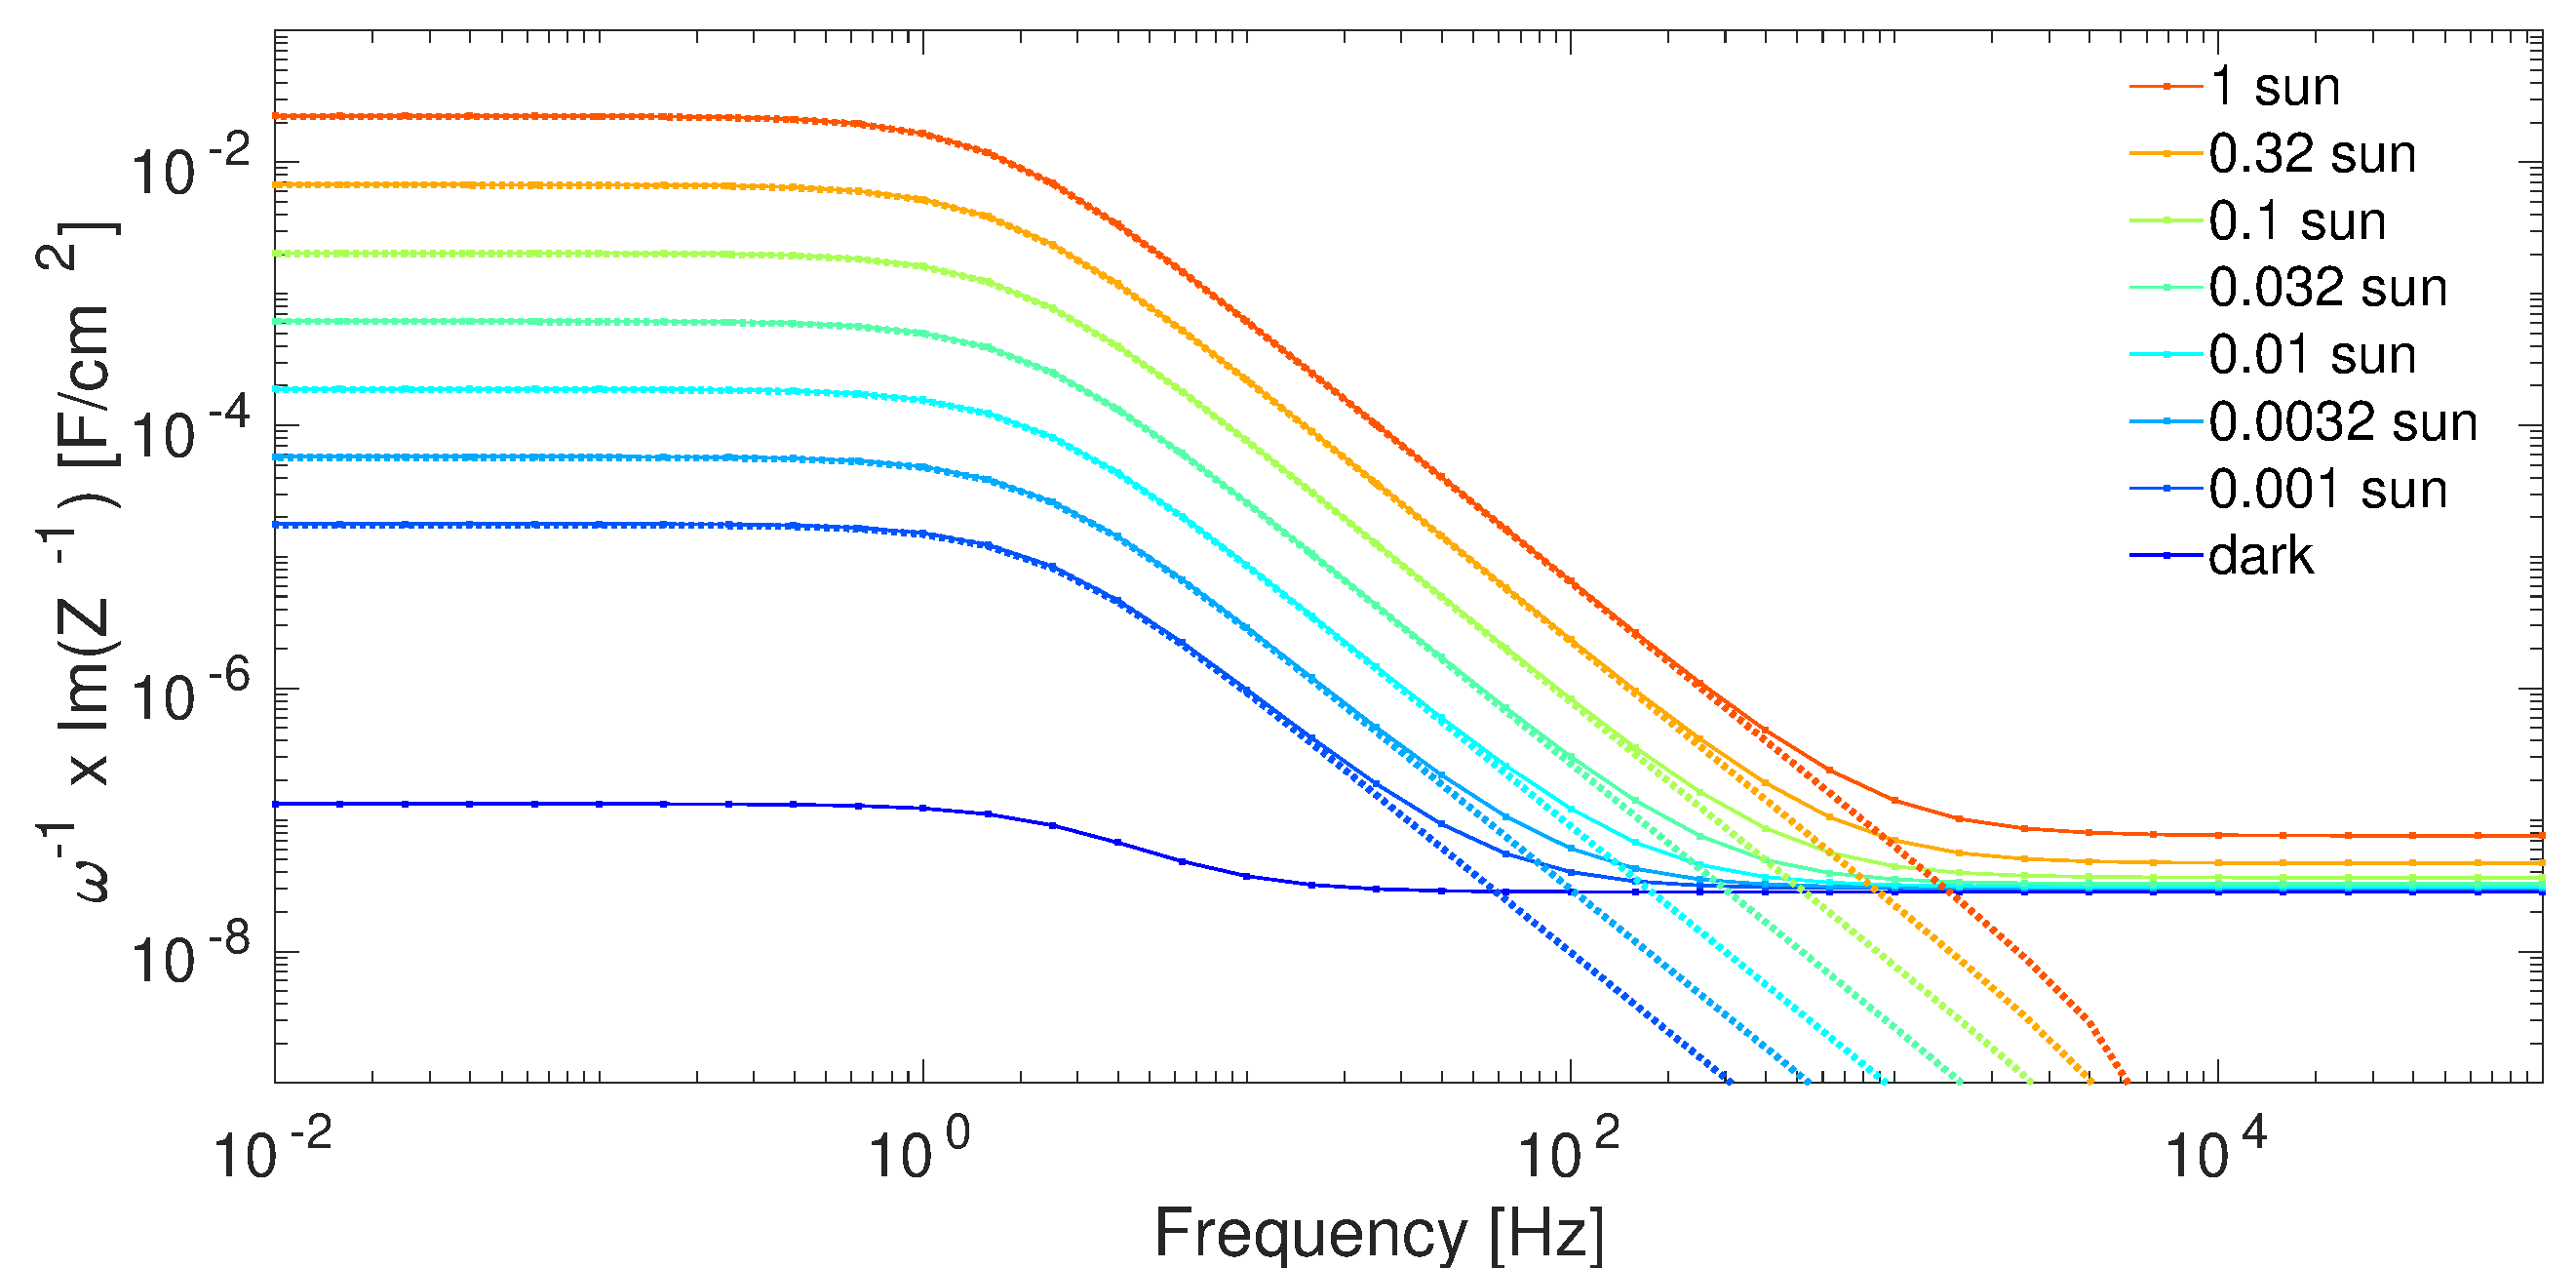
\includegraphics[width=0.9\textwidth]{dd_capacitance/recombination.pdf}
				\subcaption{Apparent capacitance from recombination current}\label{fig:impedance-recombination}
			\end{subfigure}
			
			\mycaption[Simulated apparent capacitance spectra and Nyquist plot compared with capacitance due to recombination current.]{
				In (\textbf{a}) the normalised Nyquist plot is reported, the normalisation factor is reported in the legend.
				The cross markers indicate the even frequency decades (\textsl{i.e.}\ from right to left \num{0.01}, \num{1}, \SI{100}{\Hz}\dots) so that the mid frequency minimum of 1~sun curve is around \SI{1000}{\Hz}.
				In (\textbf{b}) the apparent capacitance spectra (solid lines) is compared with the capacitance calculated from the out\hyp{}of\hyp{}phase recombination flux (dotted lines).
			}\label{fig:impedance-recombination_nyquist}
		}
	}
\end{figure}

	\paragraph{Illuminated case -- Minority carriers density point of view}
The same concept can also be understood thinking about carriers concentrations rather than energy barriers.
As represented in \cref{fig:holes_concentration}, the distance of the quasi\hyp{}Fermi level from the corresponding band level indicates the density of the corresponding carrier.
In \cref{fig:diode_transistor-band_diagram_hifreq,fig:diode_transistor-band_diagram_lowfreq} the vertical arrows indicate the distance of conduction band quasi\hyp{}Fermi level from conduction band, the closer the higher the electrons concentration.
The position of the arrows is the interface between the \textit{p}-type and the perovskite layer, so it is the region where the surface recombination annihilates electrons in the perovskite with the holes majority carriers in the \gls{htm}.
As we saw in \cpageref{intro_surface_recombination}, the surface recombination is driven by the amount of "minority" carriers, that in this case are the electrons.
The variation of the ionic species accumulation at the interface, simply due to ions electrostatic effect attracts or repels the electronic charges changing their concentration and ultimately modulating the surface recombination.
It is important to remember that the recombination flux is always present, especially when no current is measured as it counterbalances the photogeneration.
The ions accumulate and deplete at the interfaces following the applied voltage but with a delay, and this induces an out\hyp{}of\hyp{}phase component to the aforementioned recombination flux.
So if the recombination flux is large, due to a high illumination intensity or a high applied voltage, also this component will be large and, if mistaken for a capacitive current, can explain the reports about giant\index{giant capacitance} capacitance.
	



	\paragraph{Loops in the positive semi-plane and large perturbations}\label{impedance-large_perturbations}
		In \authoryear{Moia2019} we showed that the failure in stabilising the device to the measurement conditions (temperature, background voltage, illumination) results in loops in the Nyquist plot positive semi\hyp{}plane.
		Additionally, a large perturbation measurement, which is a wide sinusoidal voltage oscillation amplitude in impedance measurements, has been simulated to also cause loops in the Nyquist plot positive semi\hyp{}plane, as represented in \cref{fig:impedance-200mV}.
		This observation comes merely from simulations, no experimental confirmation is available yet.
		%But artefacts could arise and cause misinterpretations.
The fact that a large voltage perturbation causes a non\hyp{}sinusoidal current output is not a problem for the measurement itself, as the lock-in amplifiers are perfectly able to extract amplitude and phase of the signal's first harmonic (as shown in \cref{fig:demodulation}), ignoring the higher harmonics.

		\begin{figure}%impedance-200mV
			\makebox[\textwidth][c]{
				\parbox{1.1\textwidth}{
					\centering
					\begin{subfigure}[t]{1.1\textwidth}\centering
						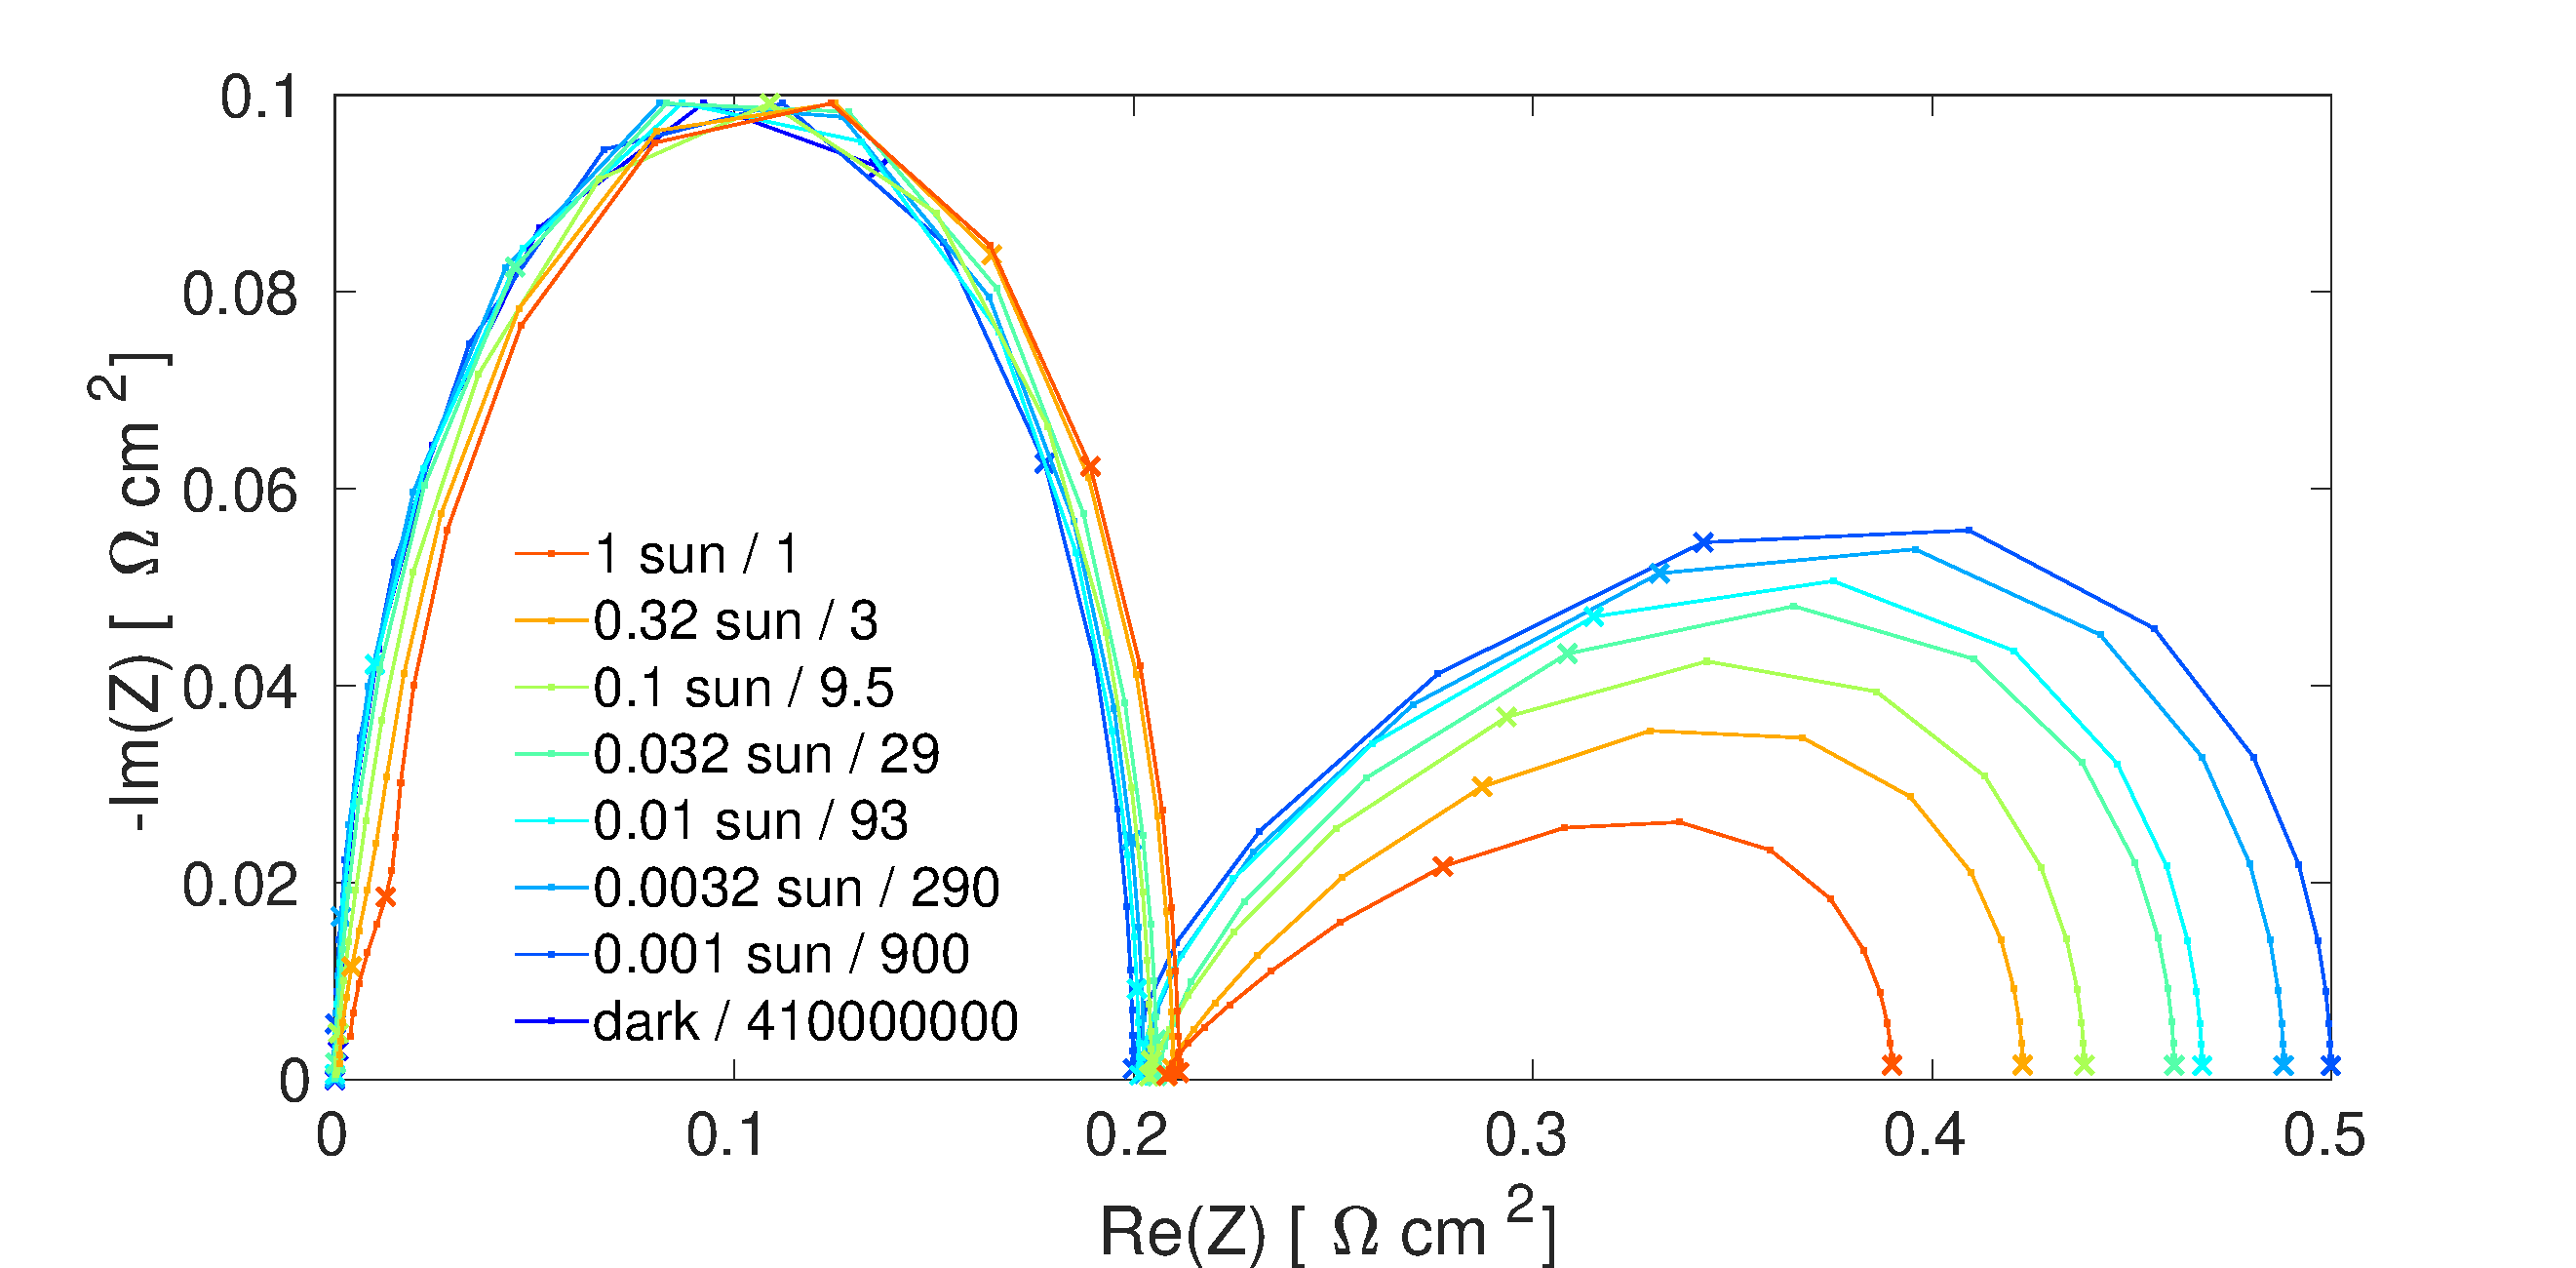
\includegraphics[width=0.8\textwidth]{dd_nyquist/nyquist_200mV_normalised.pdf}
						\subcaption{Nyquist plot with large perturbations}\label{fig:impedance-200mV_nyquist}
					\end{subfigure}
					\bigskip

					\begin{subfigure}[t]{1.1\textwidth}\centering
						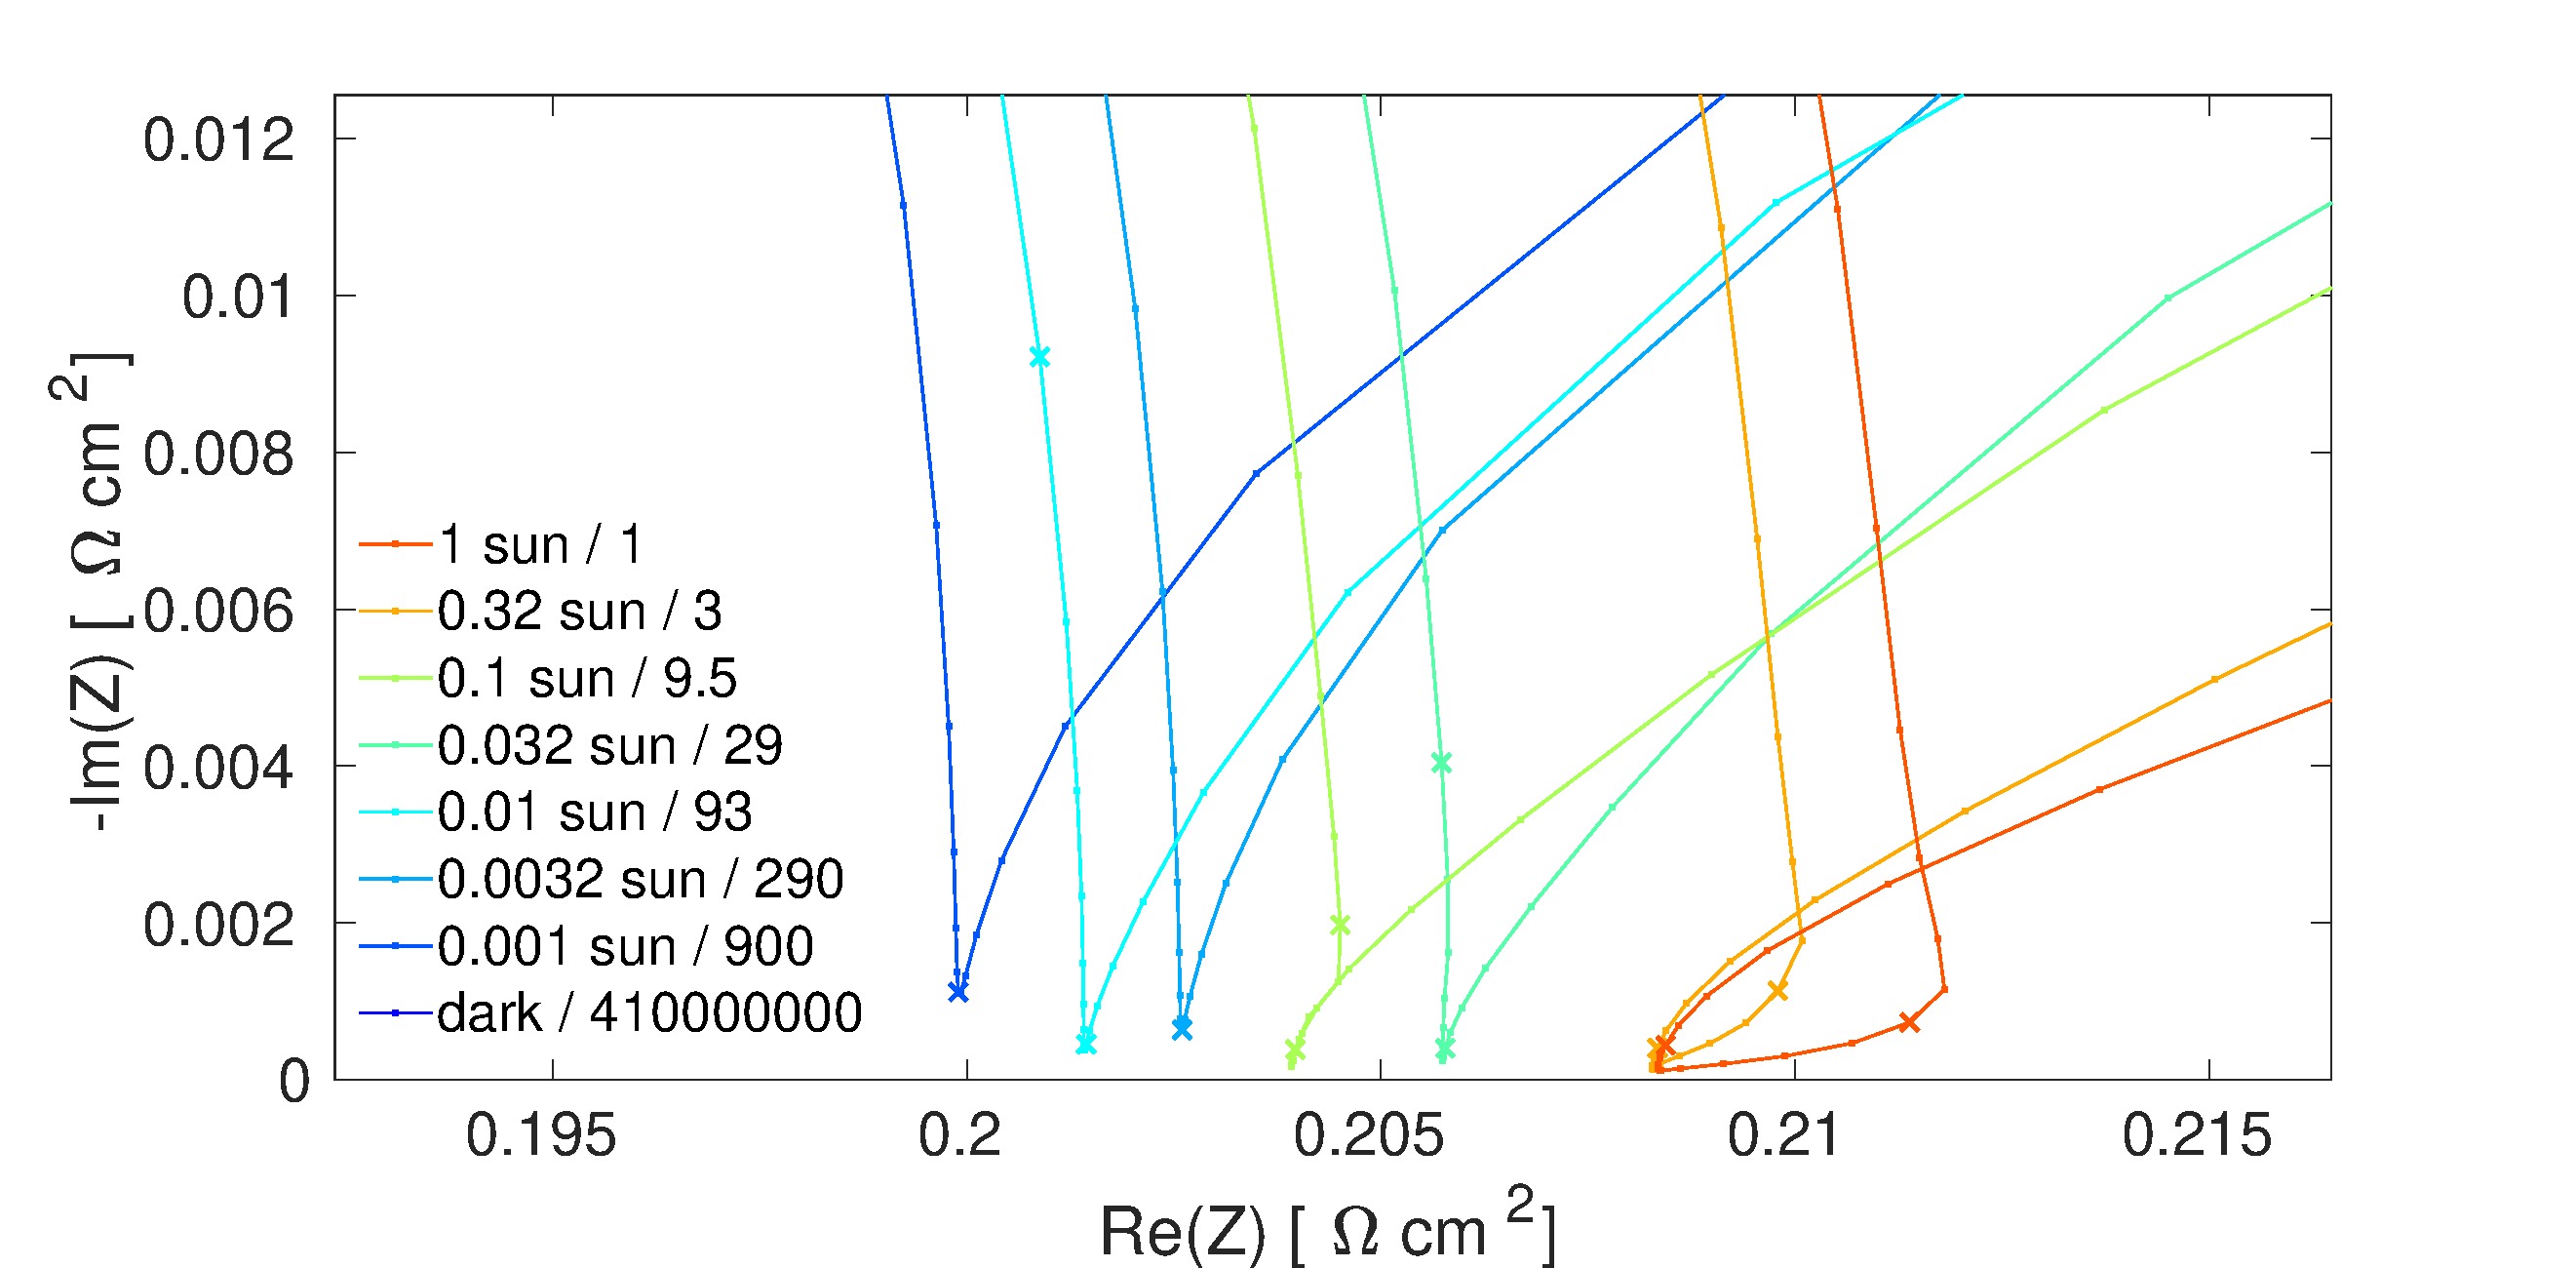
\includegraphics[width=0.8\textwidth]{dd_nyquist/nyquist_200mV_normalised_zoom.pdf}
						\subcaption{Zoom into mid frequency region}\label{fig:impedance-200mV_nyquist-zoom}
					\end{subfigure}
					\mycaption[Simulated Nyquist plot for large perturbations simulation.]{
						In (\textbf{a}) the normalised Nyquist plot of a simulation with \SI{200}{\mV} wide oscillating voltage is represented.
						Normalisation factor is indicated in the legend.
						In (\textbf{b}) zoom at mid frequencies region of the same Nyquist plot, where loops can be observed in the high intensity curves.
					}\label{fig:impedance-200mV}
				}
			}
		\end{figure}


		\mysection[Comparison of simulation and experiment]{Comparison of simulated and experimental impedance spectra}
		


		\begin{figure}%experimental
			\makebox[\textwidth][c]{
				\parbox{1.1\textwidth}{
					\centering
					\begin{subfigure}[t]{0.51\textwidth}\centering
						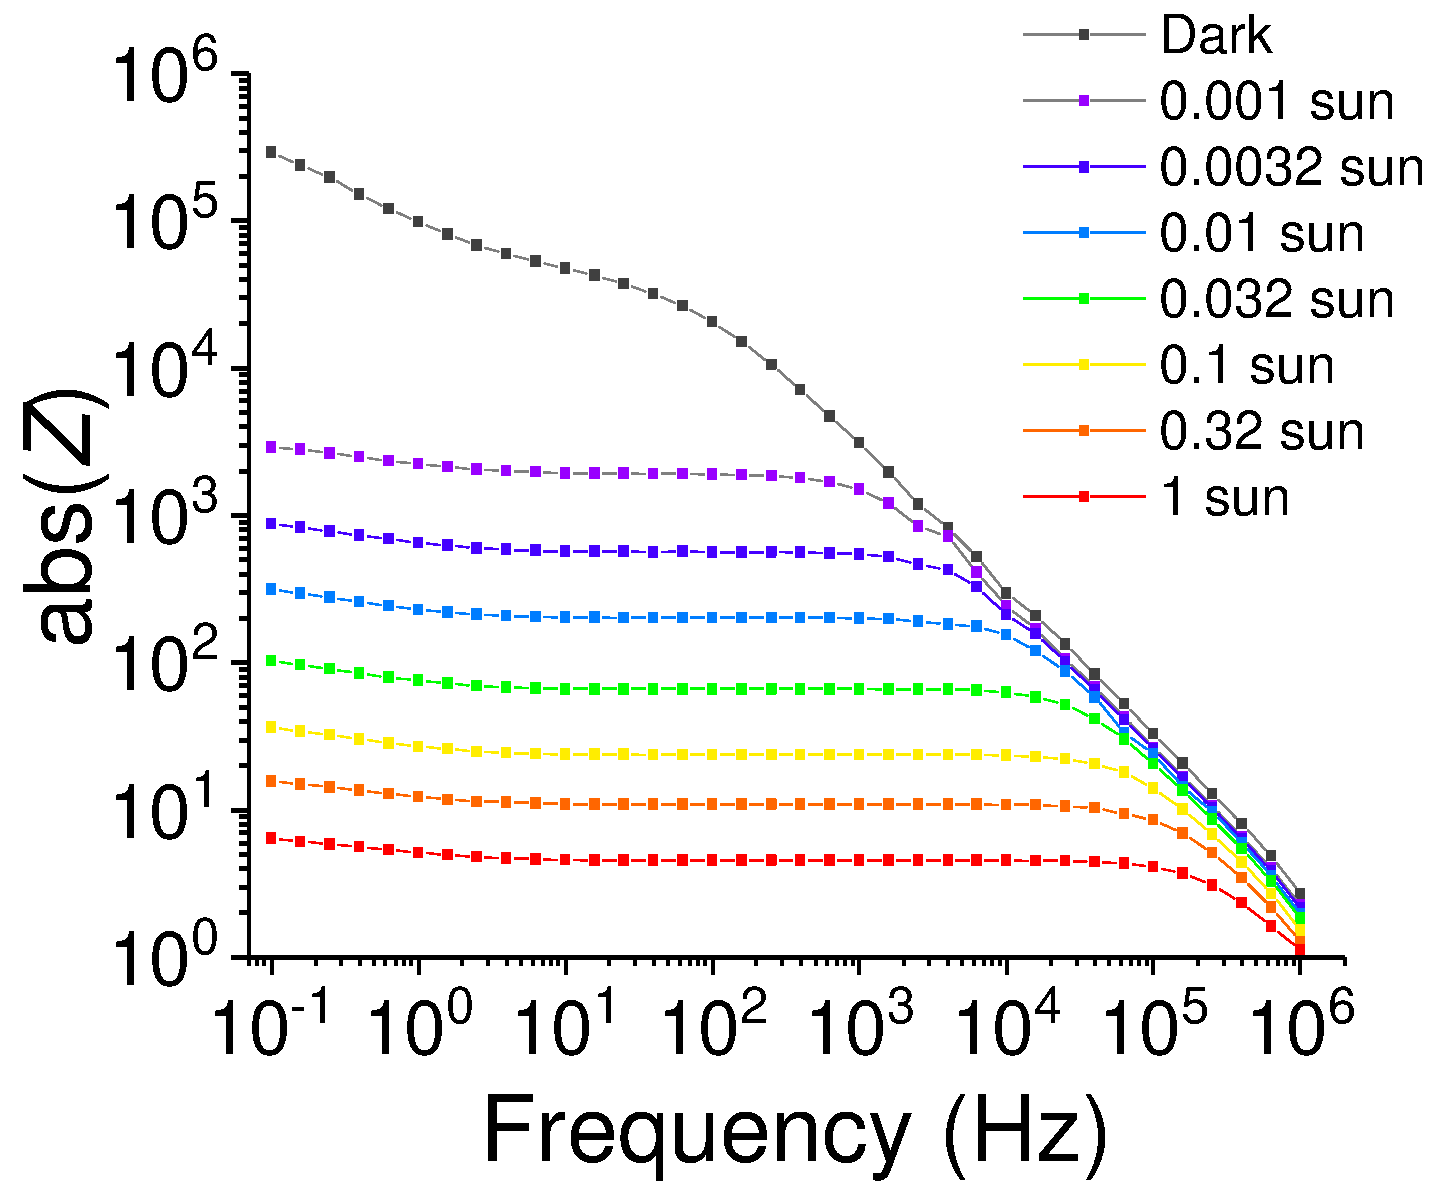
\includegraphics[width=0.9\textwidth]{experimental/Zabs-experimental.pdf}
						\subcaption{Impedance magnitude}\label{fig:experimental-Zabs}
					\end{subfigure}
					\qquad
					\begin{subfigure}[t]{0.51\textwidth}\centering
						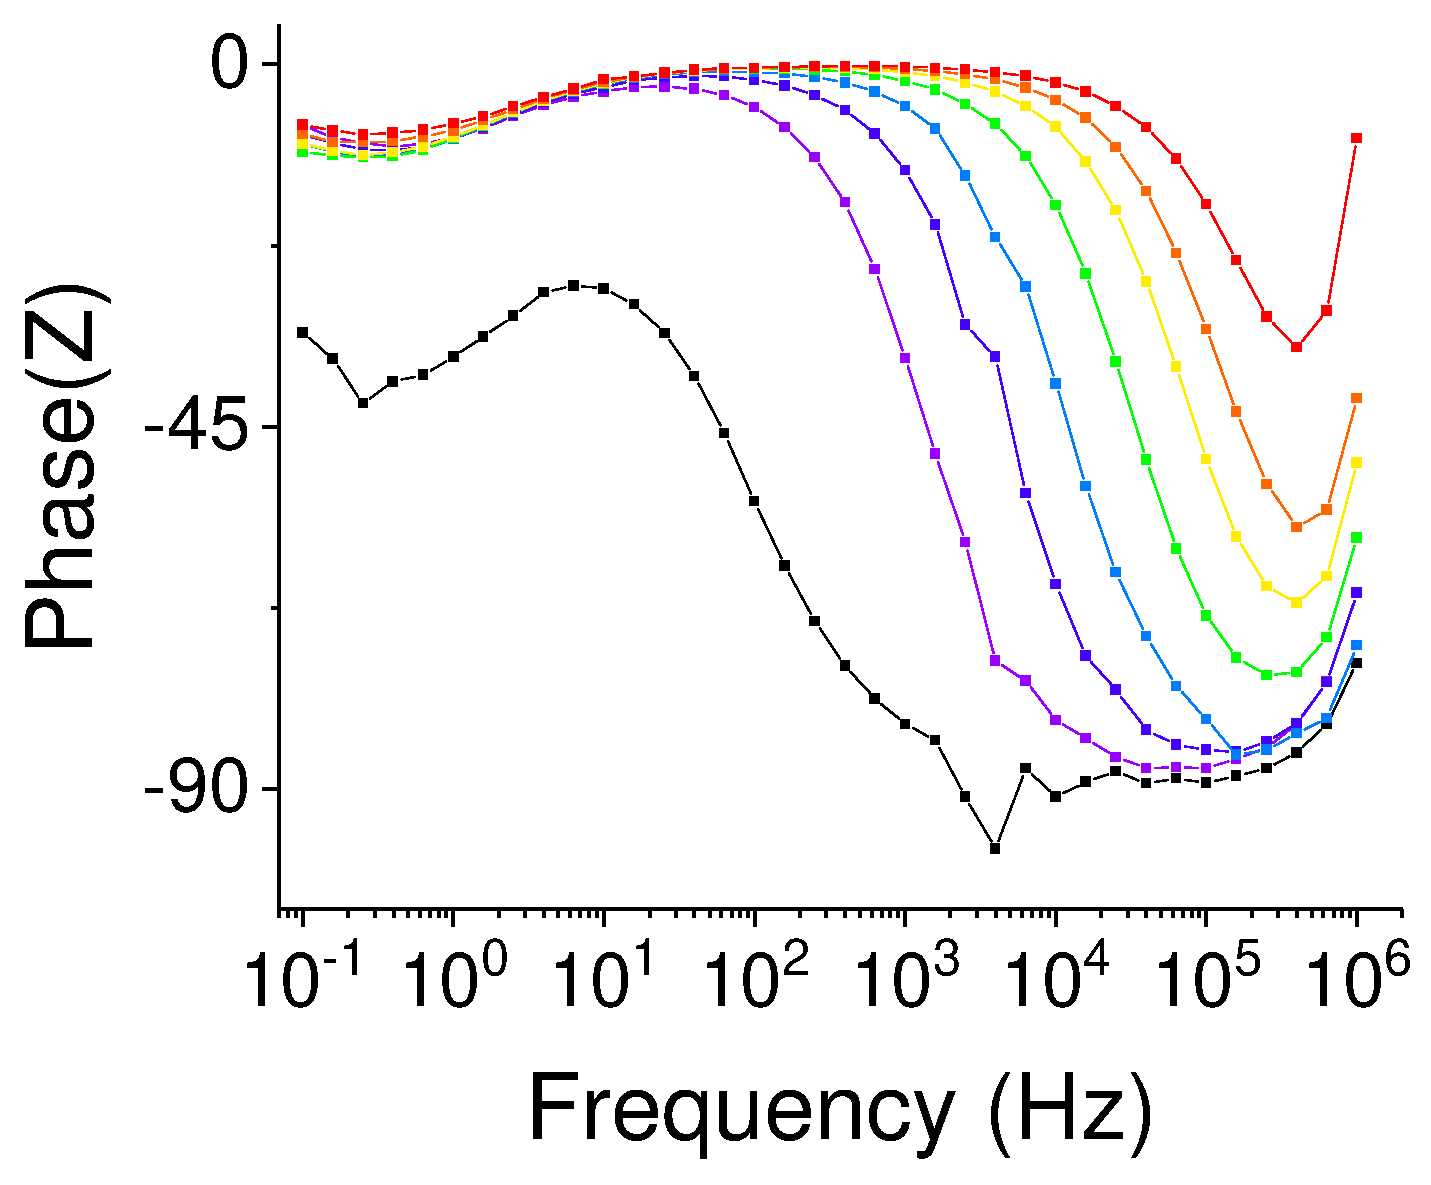
\includegraphics[width=0.9\textwidth]{experimental/phase-experimental.pdf}
						\subcaption{Impedance phase}\label{fig:experimental-phase}
					\end{subfigure}
					\bigskip

					\begin{subfigure}[t]{0.6\textwidth}\centering
						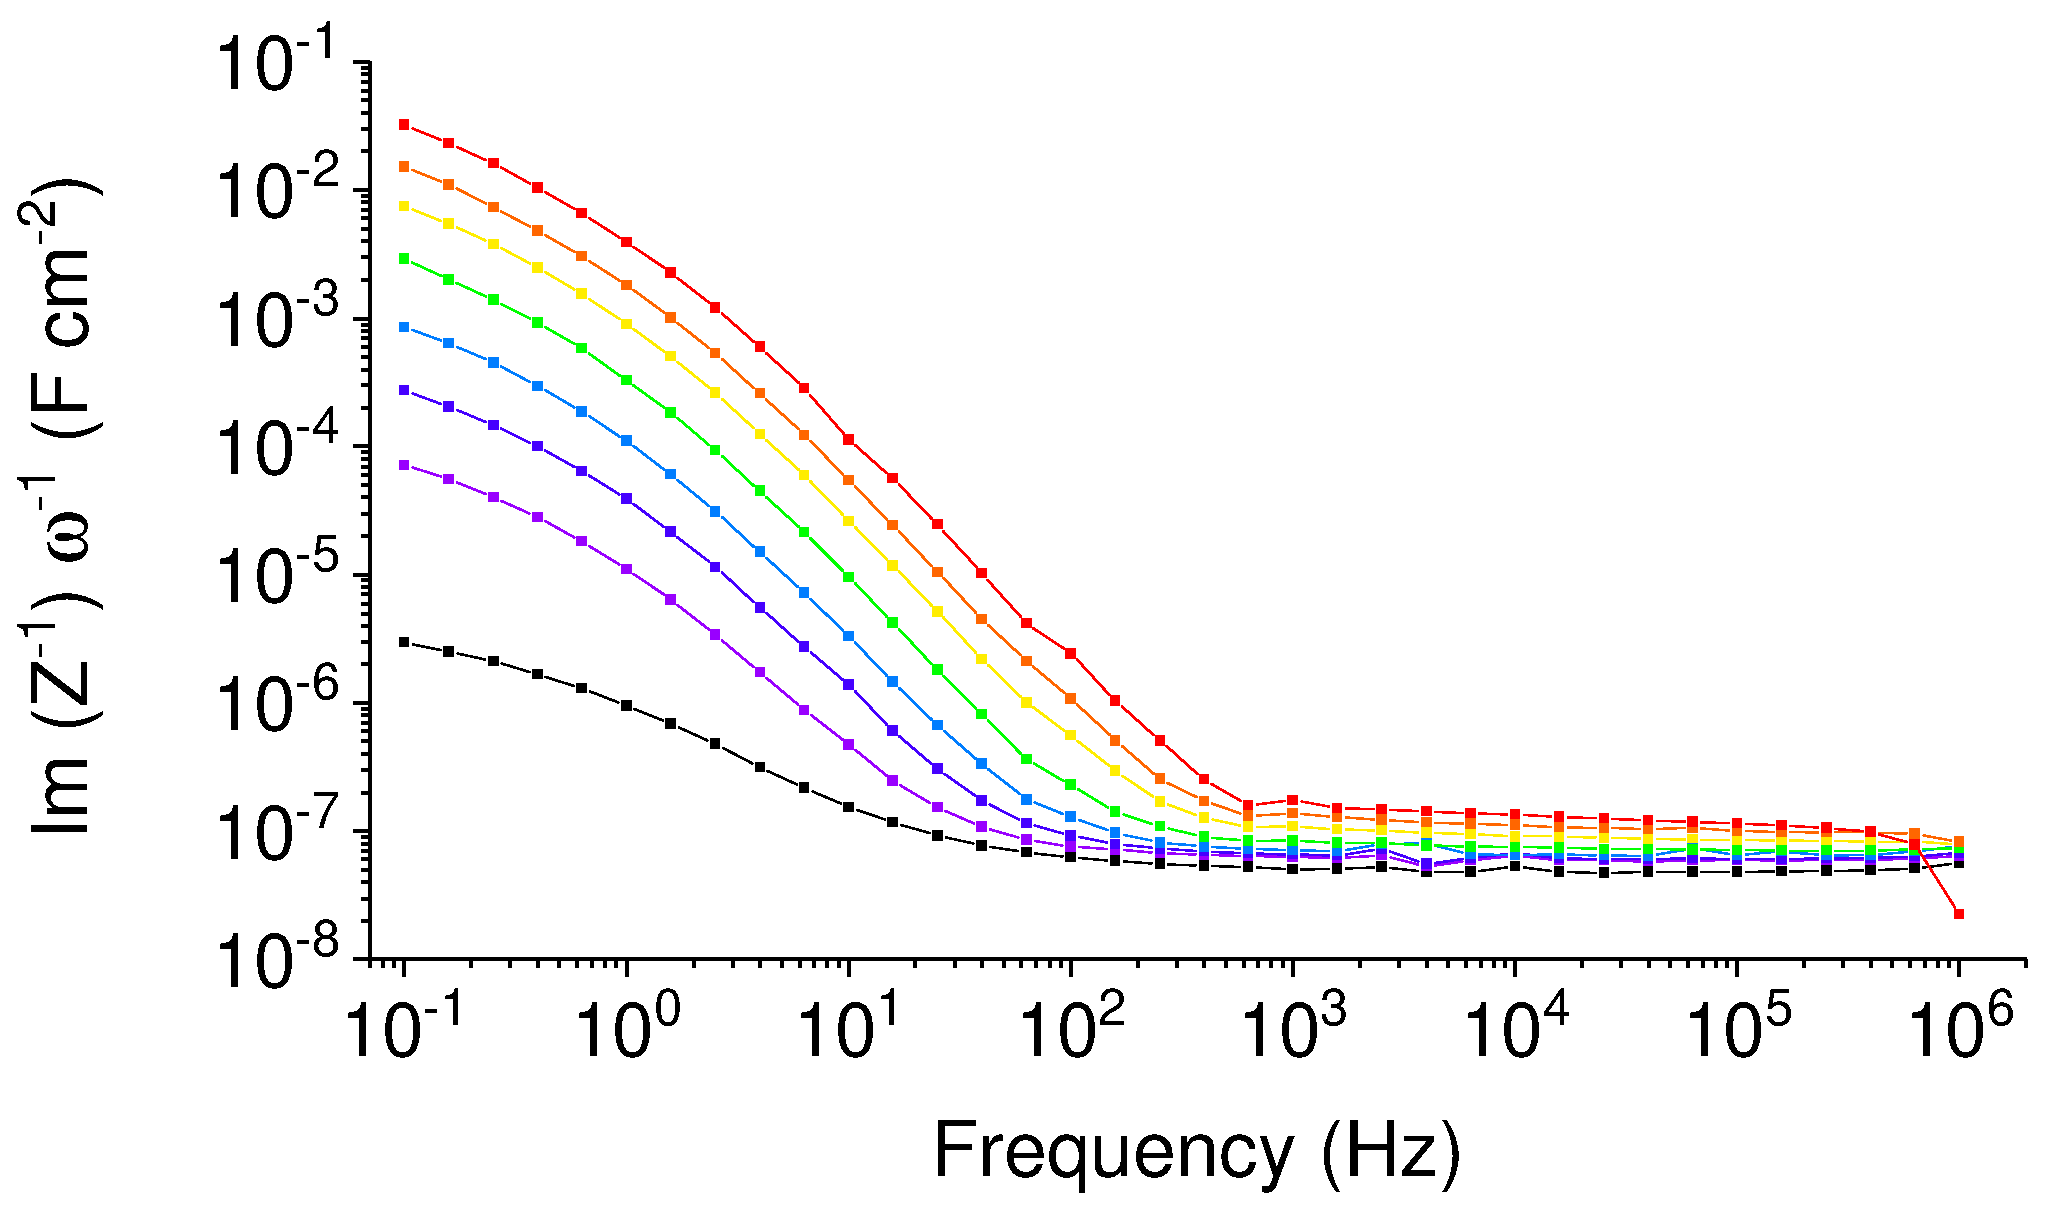
\includegraphics[width=1\textwidth]{experimental/cap-experimental.pdf}
						\subcaption{Apparent capacitance}\label{fig:experimental-cap}
					\end{subfigure}
					\qquad
\begin{subfigure}[t]{0.42\textwidth}\centering
	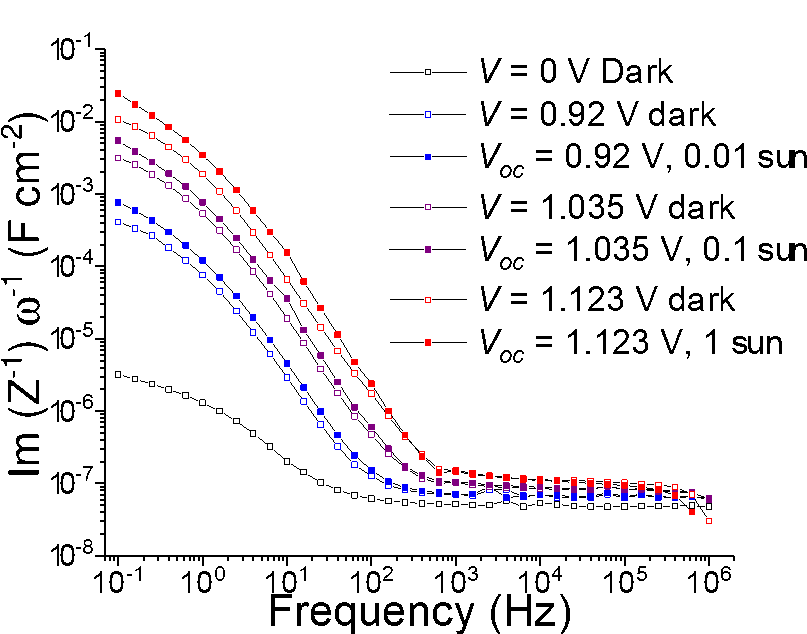
\includegraphics[width=1\textwidth]{experimental/eis-light_bias_vs_vapp2.png}
	\subcaption{Impedance phase}\label{fig:experimental-vapp}
\end{subfigure}
					\mycaption[Experimental data from impedance spectroscopy.]{
						In (\textbf{a}) the absolute value of the experimental impedance of an illuminated perovskite solar cell at open circuit conditions is reported.
						In (\textbf{b}), for the same conditions, the phase of the experimental impedance is reported, it can be compared with simulated data in \cref{fig:impedance-ionic-phase}.
						In (\textbf{c}), for the same conditions, the experimental apparent capacitance is reported, it can be compared with simulated data in \cref{fig:impedance-capacitance}.
						In (\textbf{d}) the apparent capacitance measured in the mentioned conditions is compared to the measurement performed in dark applying a voltage bias $V_|DC|$ equal to the measured light bias.
						These experimental data are courtesy of Dr.\ Davide Moia and Dr.\ Piers Barnes.
					}\label{fig:experimental}
				}
			}
		\end{figure}

		\paragraph{Lack of low frequency plateau}
		Simulating down to very low frequency we observe a plateau in the apparent capacitance, which, as shown in \cref{fig:experimental-cap,fig:experimental-vapp}, experimentally is not usually observed \cite{Juarez-Perez2014} with a few exceptions \cite{Ebadi2019}.
		The lack of a plateau has been interpreted by \authoryear{Jacobs2018} with the presence of more than one mobile ionic species, which is quite likely as seen in \cpageref{intro_ionic_migration}.
		Additionally, we hypothesized \cite{Moia2019} that this effect could arise from the different ionic mobility in perovskite when infiltrated in mesoporous layers; dispersive transport in disordered material regions \cite{Schwarz1998} where the mobility varies over time and position; or mostly diffusive transport of ions in the mesoporous layers which could be better described by a Warburg diffusion element in the equivalent electrical circuit.
		
		%\paragraph{Larger ionic capacitance}

		\paragraph{Short circuit}
		Both the simulation at open circuit with illumination or at dark with applied background voltage bias matches quite nicely the experimental data.
		On the contrary, the simulation at short circuit with illumination showed a low frequency apparent capacitance increase of just 30 times from dark to 1~sun, while experimentally a giant\index{giant capacitance} capacitance is also observed.
		This discrepancy is left unexplained, a closer look is needed in order to understand which physical phenomena is not implemented in the model or, more simply, which variable is far from the realistic value.
		Indeed, when using the more advanced heterojunction version of Driftfusion, an increase of \num{\approx 50000} times has been observed between the dark and the \SI{1}{sun} case at low frequency (and no negative capacitance\index{negative capacitance}), which is closer to the experimental observation.



\section{Further development}


\begin{figure}
	\makebox[\textwidth][c]{
		\parbox{1.1\textwidth}{
			\centering
			\begin{subfigure}[t]{1.1\textwidth}
				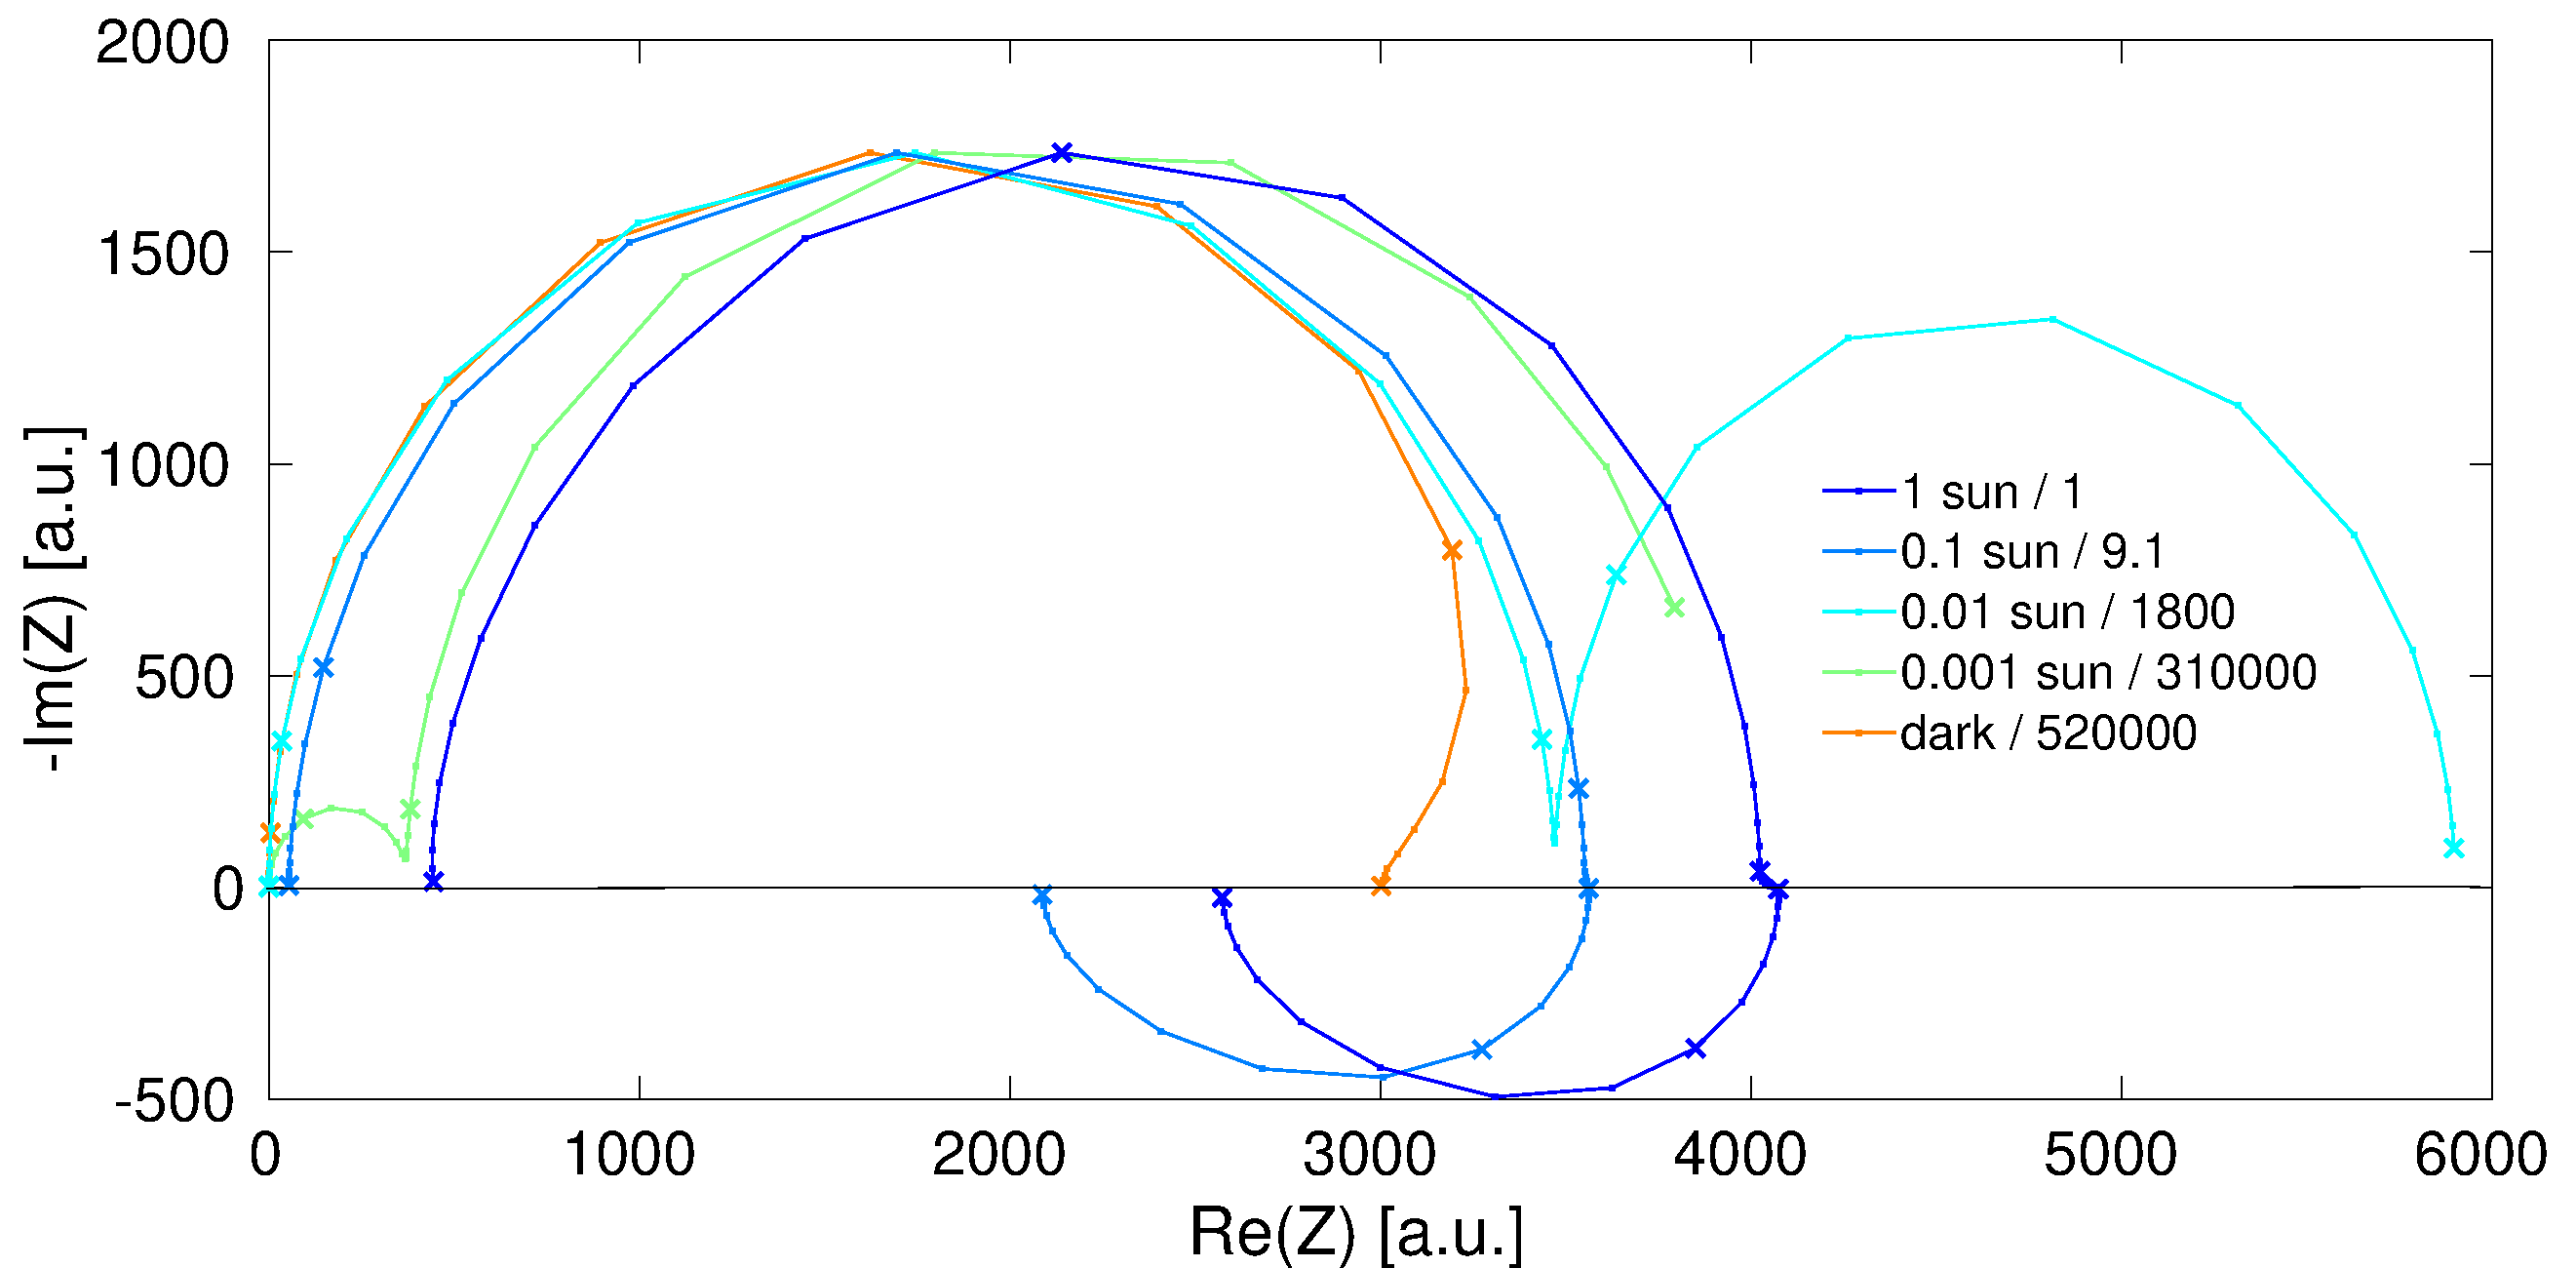
\includegraphics[width=1\textwidth]{heterojunction/ISwave_oc_nyquist_norm.pdf}
				\subcaption{Illuminated, open circuit, Nyquist}\label{fig:impedance_heterojunction-oc-nyquist}
			\end{subfigure}
			%			\qquad
			\bigskip
			
			\begin{subfigure}[t]{1.1\textwidth}
				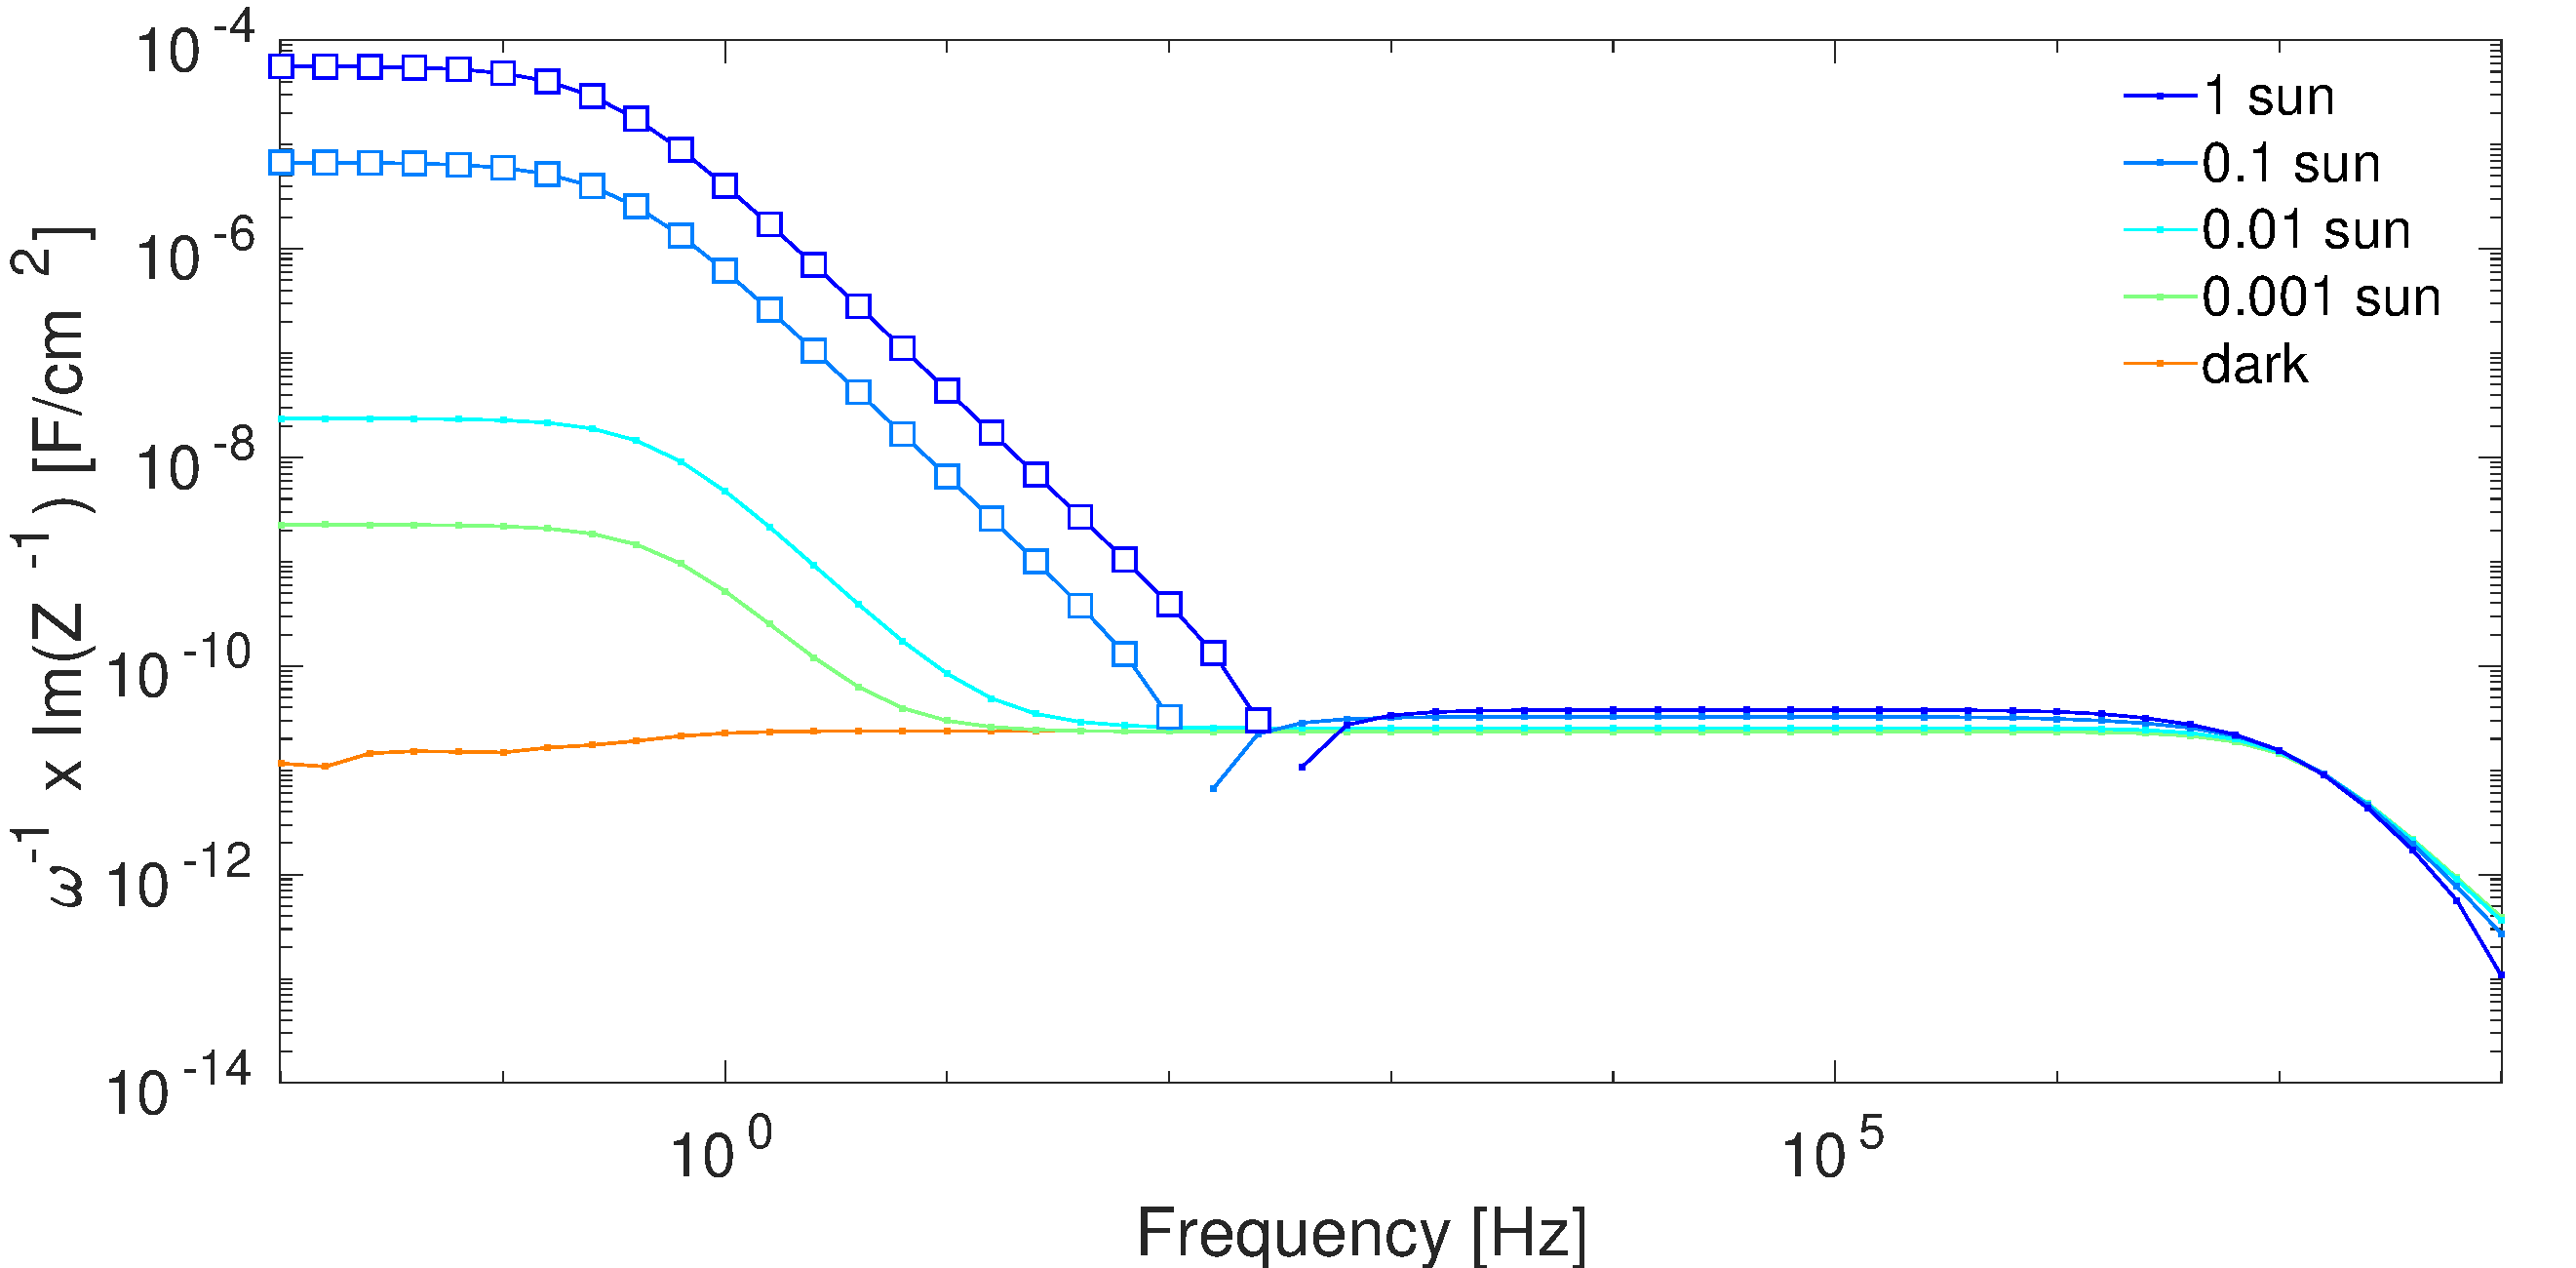
\includegraphics[width=1\textwidth]{heterojunction/ISwave_oc_cap.pdf}
				\subcaption{Illuminated, open circuit, apparent capacitance}\label{fig:impedance_heterojunction-oc-cap}
			\end{subfigure}
			%			\bigskip
			%			
			%			\begin{subfigure}[t]{0.51\textwidth}
			%				\includegraphics[width=1\textwidth]{heterojunction/ISwave_Vapp_nyquist_norm.png}
			%				\subcaption{Dark, applied voltage, Nyquist}\label{fig:impedance_heterojunction-vapp-nyquist}
			%			\end{subfigure}
			%						\qquad
			%			\begin{subfigure}[t]{0.51\textwidth}
			%				\includegraphics[width=1\textwidth]{heterojunction/ISwave_Vapp_cap.png}
			%				\subcaption{Dark, applied voltage, apparent capacitance}\label{fig:impedance_heterojunction-vapp-cap}
			%			\end{subfigure}
			\mycaption[Preliminary simulations of impedance on heterojunction model.]{The filled symbols indicate positive capacitance values, the hollow symbols represents negative capacitance\index{negative capacitance} which was changed in sign in order to be plotted on the same axis.}\label{fig:impedance_heterojunction}
		}
	}
\end{figure}

\paragraph{Heterojunction}
The simulations shown here are all based on a \textit{p-i-n} homojunction model, so a proper injection barrier could not actually be simulated and the negative capacitance\index{negative capacitance} we reported in \authoryear{Moia2019} has been obtained playing with extreme values of the mobility and recombination parameters.
An attempt of adapting the impedance scripts to the most recent heterojunction version of Driftfusion confirmed the presence of negative capacitance\index{negative capacitance} due to injection barrier modulation by ionic charge, as shown in \cref{fig:impedance_heterojunction}.
This confirms that our hypothesis of the ionically modulated injection barrier can be used for explaining the experimentally observed negative capacitance\index{negative capacitance} \cite{Guerrero2016,Moia2019,Ghahremanirad2017,Sanchez2014}
Further work is needed for completely adapting the impedance scripts to the upstream heterojunction core code.

\paragraph{Complete simulation of ElectroAbsorbance}
We refer with the names of ElectroAbsorbance or Stark spectroscopy to the absorbance variation caused by an oscillating applied voltage, as described by the Franz\hyp{}Keldysh effect.
This effect stems from the higher absorptivity of a material in presence of an electric field.
This simulation has already been implemented but the code release is waiting for the publication of the related work; the description of the modules is already available in \cpageref{software_electroabsorbance}.

\paragraph{Implement other similar techniques}
Using some of the modules already implemented for impedance spectroscopy simulation, it should be easy to implement also other characterisation techniques like Intensity-Modulated Photovoltage/Photocurrent Spectroscopy (IMVS, IMPS) \cite{Pockett2015,Guillen2014} and Mott-Schottky capacitance analysis \cite{Almora2016}.

\paragraph{Faster simulation with voltage step}\label{impedance_fourier}
The first implementation of the impedance spectroscopy simulation done in November 2017 did not employ the complete description of the oscillating voltage.
Just a voltage step was applied and the resulting current evolution was used for obtaining a rough approximation of the apparent capacitance spectrum.
This approach is computationally much faster than a complete oscillating simulation and can give exactly the same results if properly treated for converting the time\hyp{}domain data to frequency\hyp{}domain using a Fourier transform.
In the publication by \authoryear{Jacobs2018}, they used this approach for simulating impedance spectroscopy in perovskite solar cells.
Our preliminary implementation needs to be refined and at this stage is not ready for being published.
Following this approach, we can obtain frequency domain simulations for IMVS, IMPS, and impedance spectroscopy respectively from \acr{tpv}, \acr{tpc}, and current\hyp{}voltage step small perturbations (see Supplementary Note 5 or Supplementary Note 4 for sweep large perturbation in \authoryear{Moia2019}) simulations in time domain.
For example, converting a bi\hyp{}exponential decay in \acr{tpv} to frequency domain through Fourier transform, we can obtain two arches in the IMVS Nyquist plot or from a bi\hyp{}exponential current evolution after a voltage step we can obtain the impedance spectroscopy features (preliminary simulation performed by Dr.\ Piers Barnes) as shown in \cref{fig:impedance_fourier}.
\authoryear{Ebadi2019} also have shown how a device showing current transient with two opposite phases will also show a negative capacitance\index{negative capacitance} in impedance spectroscopy.
Similarly, for current\hyp{}voltage sweeps I suppose that the "bumps" (see \cpageref{characterization_scanspeed} and \cref{fig:iv_ugly}) and the "negative hysteresis" (forward sweep giving a higher maximum \gls{pce} than reverse sweep) which can be observed for some perovskite solar cells at certain scan speeds are also indicative of the presence of negative capacitance\index{negative capacitance} in these devices.

\begin{figure}
	\makebox[\textwidth][c]{
		\parbox{1.1\textwidth}{
			\centering
			\begin{subfigure}[t]{0.45\textwidth}
				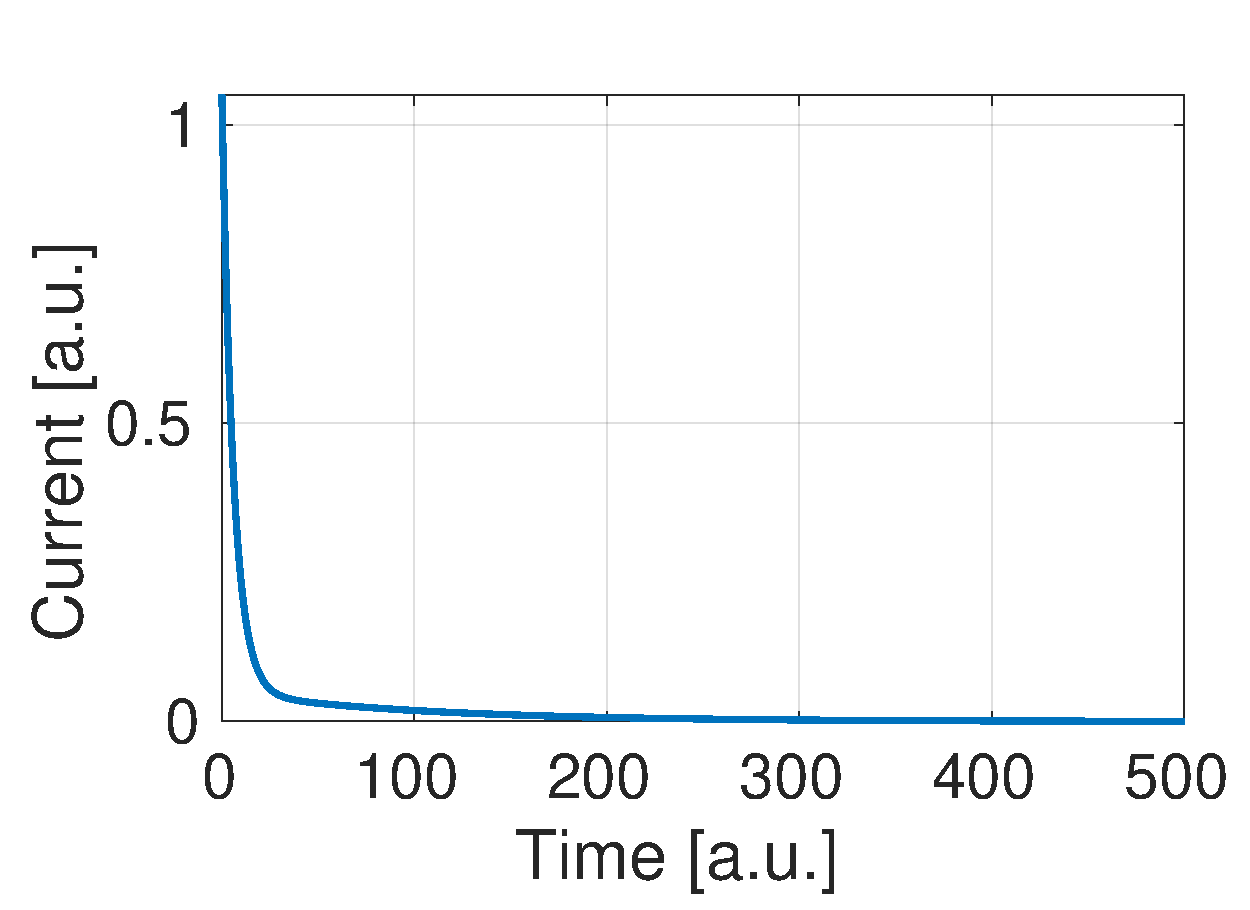
\includegraphics[width=1\textwidth]{fourier/posSlowExp.pdf}
				\subcaption{Bi-exponential decay}\label{fig:impedance_fourier_posSlowExp}
			\end{subfigure}
			\qquad
			\begin{subfigure}[t]{0.45\textwidth}
				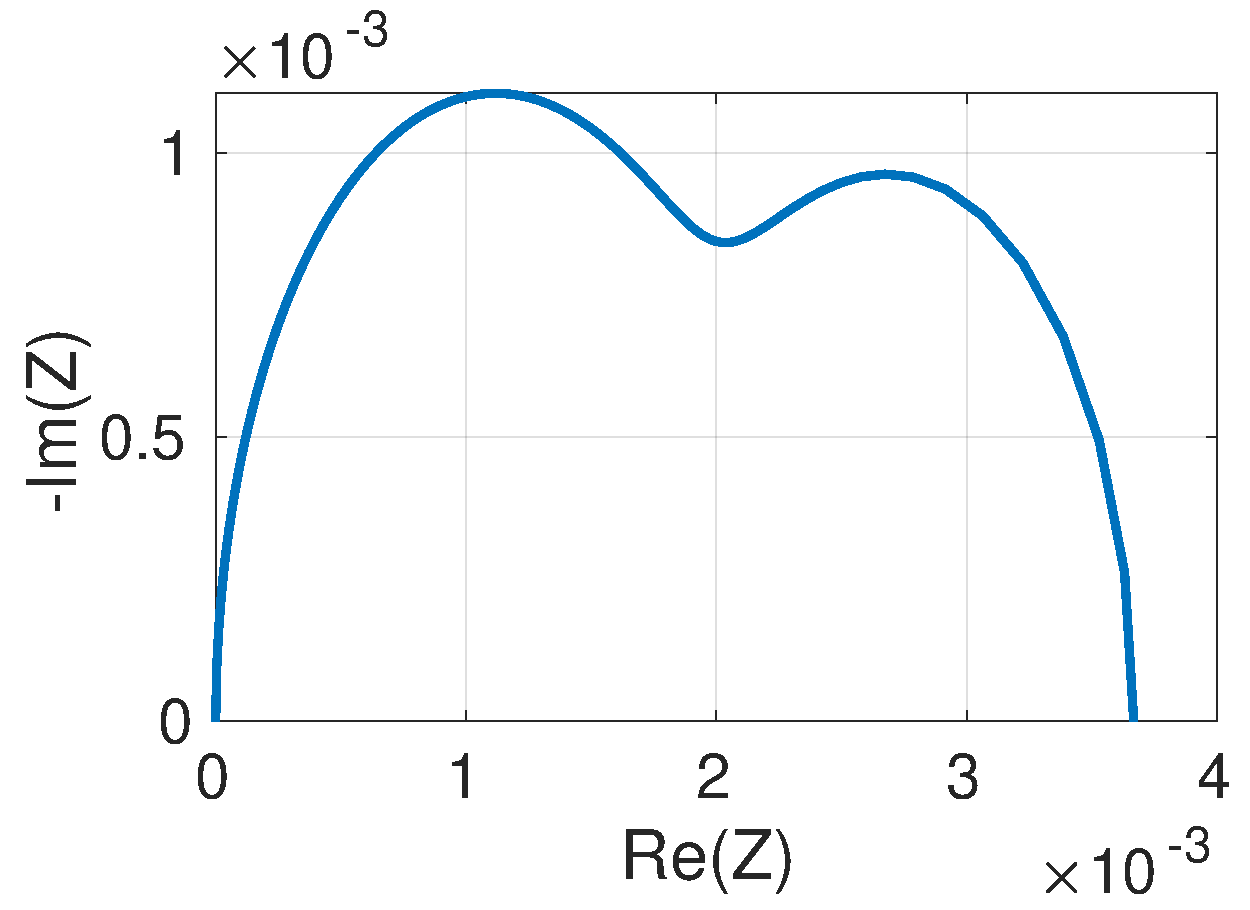
\includegraphics[width=1\textwidth]{fourier/impsig-posSlowExp.pdf}
				\subcaption{Frequency domain representation}\label{fig:impedance_fourier_impsig-posSlowExp}
			\end{subfigure}
			\bigskip
			
			\begin{subfigure}[t]{0.45\textwidth}
				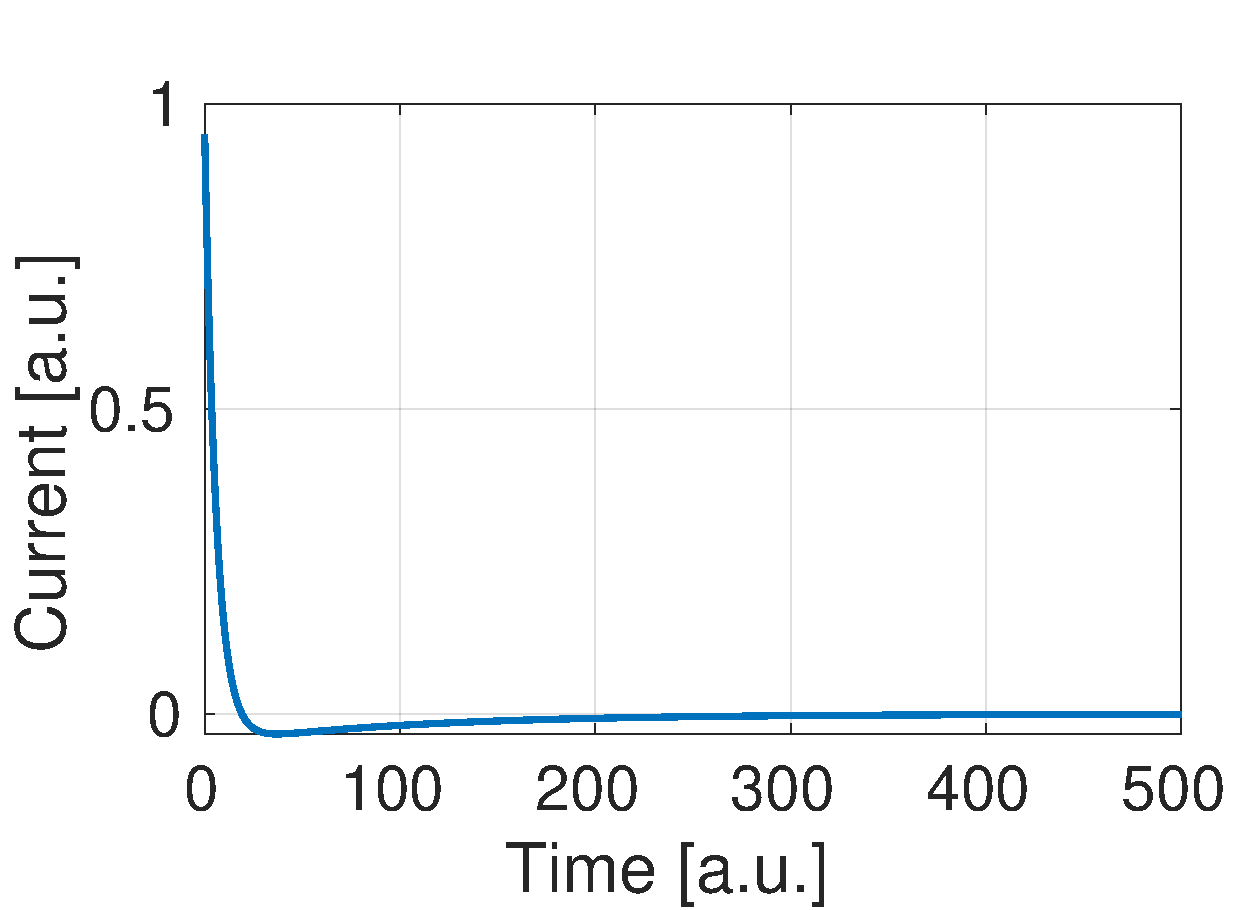
\includegraphics[width=1\textwidth]{fourier/negSlowExp.pdf}
				\subcaption{Positive fast decay and negative slow decay}\label{fig:impedance_fourier_negSlowExp}
			\end{subfigure}
			\qquad
			\begin{subfigure}[t]{0.45\textwidth}
				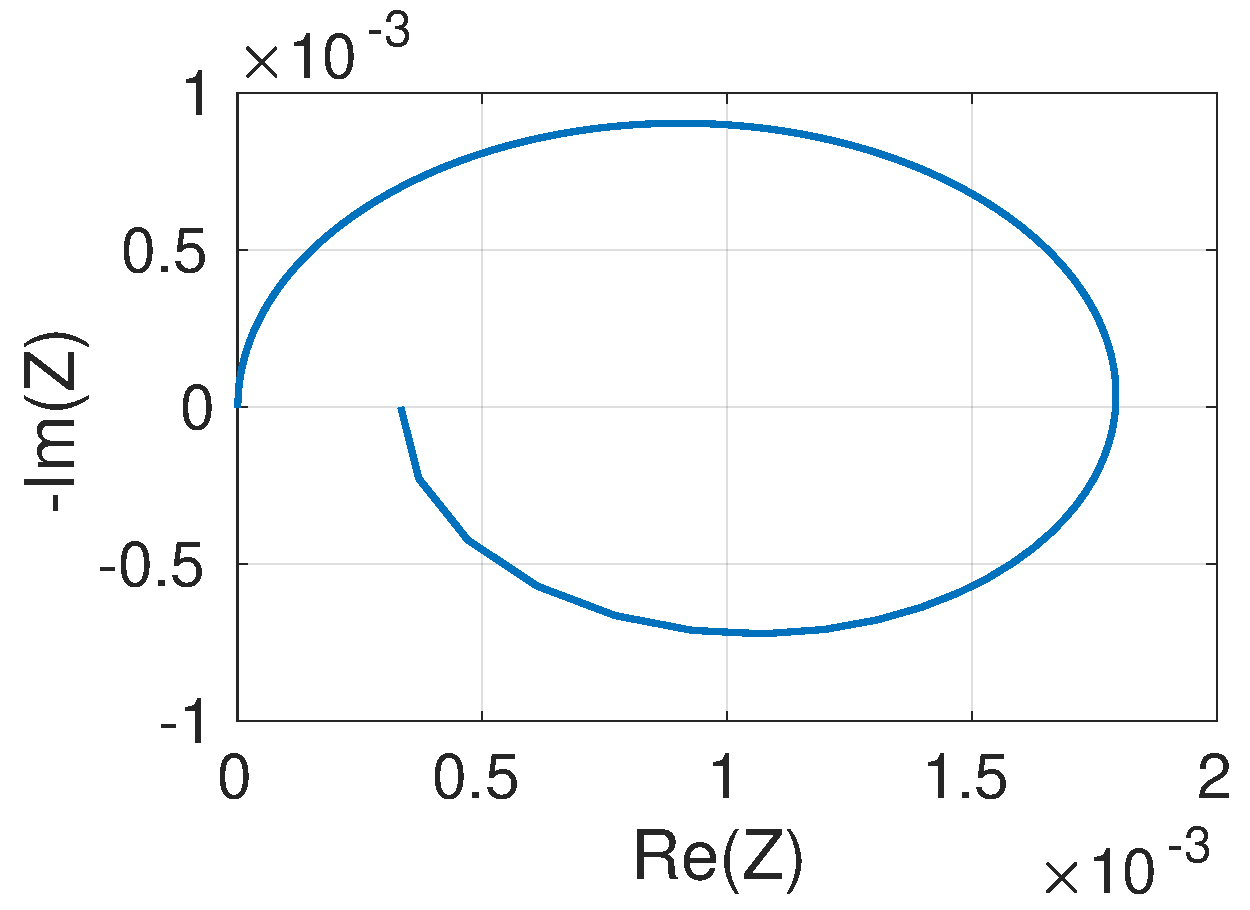
\includegraphics[width=1\textwidth]{fourier/impsig-negSlowExp.pdf}
				\subcaption{Frequency domain representation}\label{fig:impedance_fourier_impsig-negSlowExp}
			\end{subfigure}
			\mycaption[Example of Fourier transformation of bi\hyp{}exponential current decays to impedance spectra.]{
				In (\textbf{a}) a bi\hyp{}exponential decay is plotted, it can be thought as the output current profile after a voltage step.
				In (\textbf{b}) the corresponding Nyquist plot is reported as obtained \textsl{via} Fourier transform, we can see how the profile in (\textbf{a}) causes the presence of two arches.
				In (\textbf{c}) another kind of bi\hyp{}exponential shape is represented, in which the slow exponential gives an increasing trend.
				In (\textbf{d}) the corresponding Nyquist plot shows that we can expect inductive effects for the case represented in (\textbf{c}).
				The employed code is courtesy of Dr.\ Piers Barnes.
			}\label{fig:impedance_fourier}
		}
	}
\end{figure}

\section{Implementation of impedance spectroscopy}

	\begin{figure}%impedance_flowchart
		\centering
		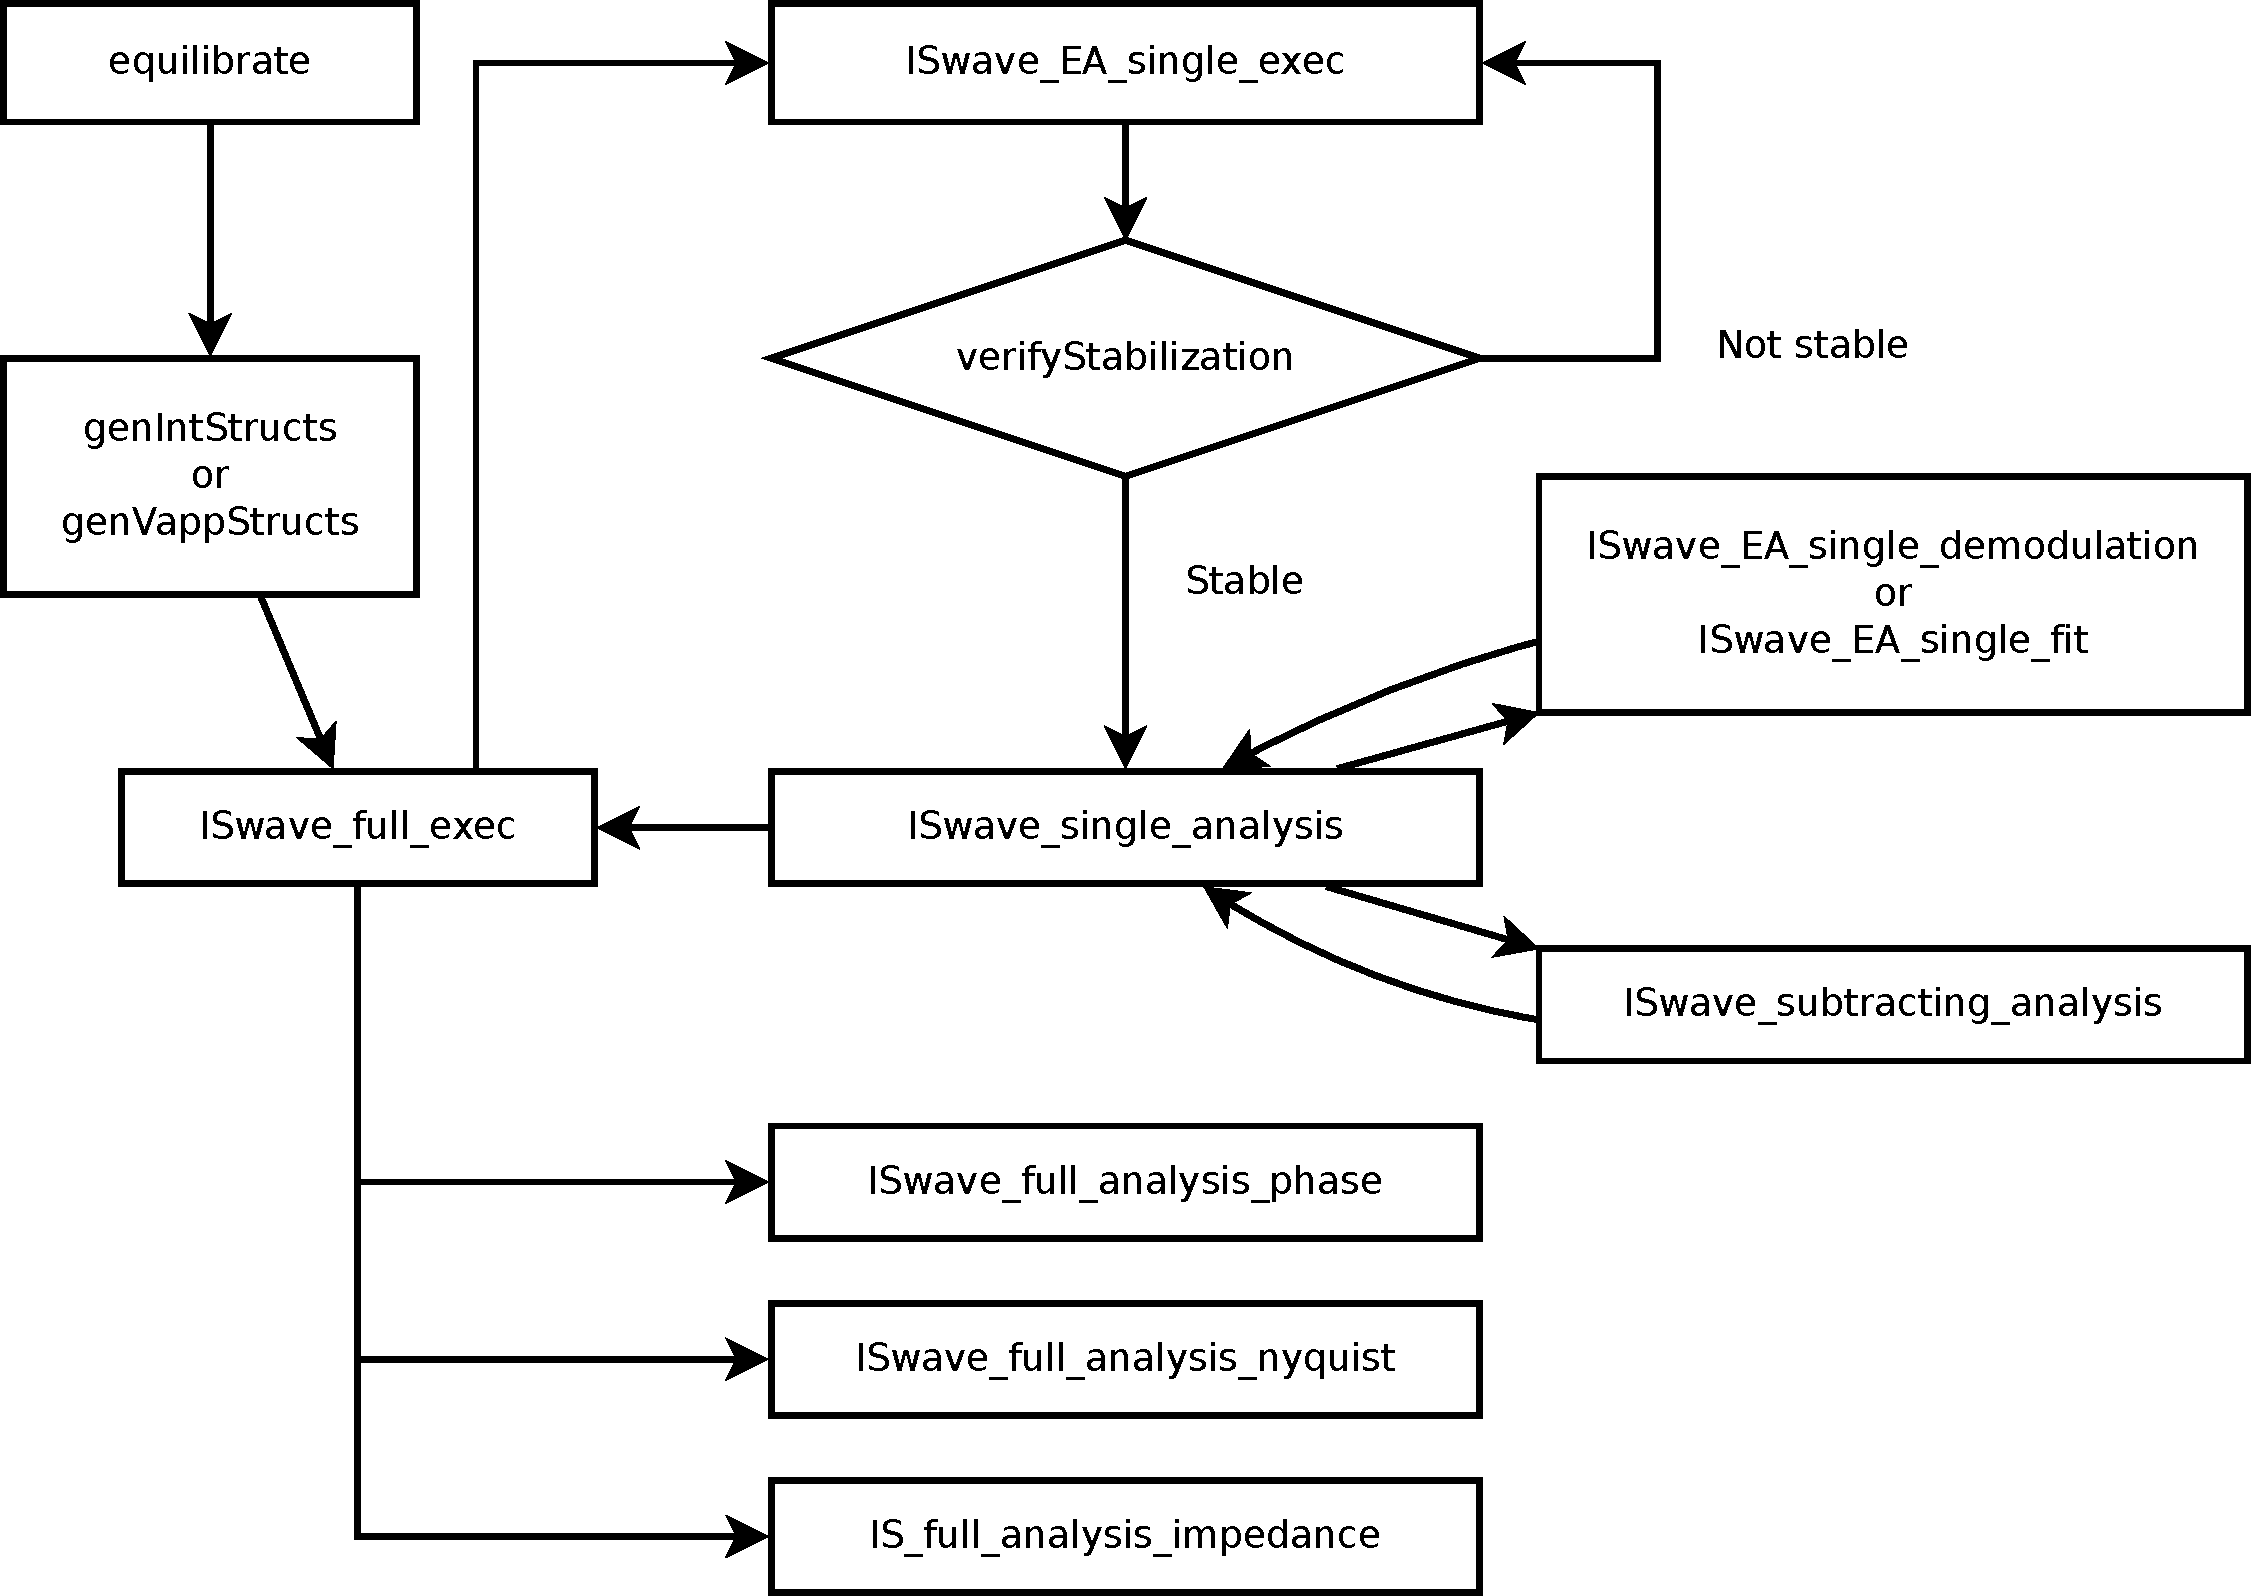
\includegraphics[width=1.05\textwidth]{flowchart/flowchart-crop.pdf}
		\mycaption[Flowchart of impedance simulation modules.]{
			The representation indicates the logical flow of the simulation, in some parts does not corresponds to the actual calls.
			Also, some of the secondary pieces have been skipped for simplicity.
			\texttt{equilibrate} is part of Driftfusion core and generates stabilised solutions, while \texttt{gen\-Int\-Structs}, \texttt{gen\-Vapp\-Structs}, and \texttt{verify\-Stabilization} are described in \cpageref{verifyStabilization,genVappStructs}.
		}\label{fig:impedance_flowchart}
	\end{figure}

	I choose to split the implementation in independent modules, so that some of them can be easily re-used for other kinds of simulations.
	The logical flowchart of a complete impedance spectra simulation has been represented in \cref{fig:impedance_flowchart}.


	\paragraph{\texttt{IS\-wave\_EA\_single\_exec} -- Does a single impedance spectroscopy simulation}
	Starting from the last time point of the provided solution it applies a time-varying voltage.
	This voltage profile is the background voltage bias from the provided solution summed to a sinusoidally oscillating voltage.

	\textit{Inputs:} 1) a single asymmetric structure as created by \texttt{pin\-drift};
	2) voltage oscillation amplitude in volts;
	3) voltage oscillation frequency;
	4) number of periods to be simulated;
	5) how many time points should the solution have for
	each period, suggested to use a multiple of 4;
	6) logical, check if the oscillating solution reached a
	(oscillating) stabilisation, otherwise just use the result of the
	initial simulation. This can be useful when it is known that the
	starting solution is not stabilised, for example measuring with an
	unstabilised ionic profile;
	7) logical, set to true when performing ElectroAbsorbance simulation,
	this will skip the electrical current calculation;
	8) starting relative tolerance of the \texttt{pdepe} solver, for example a
	value of \num{1e-8} sets for a very precise simulation.

	\textit{Outputs:} a structure with a solution being perturbed by an
	oscillating voltage.

	\textit{Requires:} \texttt{pin\-drift}, \texttt{verify\-Stabilization}, \texttt{pinana}.

	\textit{Required by:} \texttt{IS\-wave\_full\_exec}, \texttt{IS\-wave\_full\_exec\_nonparallel}, \texttt{EA\_full\_exec}.

	\textit{Example:} using \texttt{asymmetricize} (see \cpageref{asymmetricize}) the symmetric solution at 1 sun illumination and open circuit is broken in halves in order to be able to apply a custom voltage.
	Then this script simulates an oscillating voltage at \SI{0.1}{\Hz} and \SI{2}{\mV} of half peak to peak voltage amplitude, with a constant voltage bias equal to the device \gls{voc},
	20 periods and 40 time points per period, taking care of reaching a stable solution,
	and using a starting relative tolerance of \num{1e-8} and calculates also the electronic current needed by impedance simulations.
	\begin{lstlisting}[style=Matlab-editor]
>> asymssol_i_1S_SR_is_100mHz_2mV = ISwave_EA_single_exec(asymmetricize(ssol_i_1S_SR), 2e-3, 1e-2, 20, 40, true, false, 1e-8)
   \end{lstlisting}

	\paragraph{\texttt{IS\-wave\_EA\_single\_demodulation} -- Calculates phase and amplitude demodulating oscillating current data from impedance spectroscopy}\label{ISwave_EA_single_demodulation}
	The current profile gets multiplied by the voltage profile and,
	separately, by the voltage profile with an additional \SI{90}{\degree} phase.
	The integrals of the resulting profiles are related to the phase.
	This simulates the working principle of a dual-phase demodulator often
	used by lock-in amplifiers.
	A phase close to \SI{90}{\degree} results in very small values of
	the in-phase integral which can have a wrong sign and result in a wrong phase of
	\SI{-90}{\degree}, in that case the simulation should be repeated with smaller \texttt{pdepe}
	relative tolerance.

	\textit{Inputs:} 1) a column with the time mesh;
	2) a column with the value to be fitted, which in case of impedance simulation is the current \textsl{versus} time profile;
	3) an anonymous function containing a constant bias, the amplitude of
	the sinusoid, its phase and the frequency;
	4) an array with the parameters used for calculating the applied
	oscillating voltage in the provided anonymous function.

	\textit{Outputs:} an array with the values from the demodulation: constant
	bias, sinusoid amplitude, phase shift.

	%		\textit{Requires:} 

	\textit{Required by:} \texttt{IS\-wave\_single\_analysis}, \texttt{EA\_single\_analysis}.


	\textit{Example:} demodulate the components of the oscillating current.
	\begin{lstlisting}[style=Matlab-editor]
>> ISwave_EA_single_demodulation(asymssol_i_1S_SR_is_100mHz_2mV.t', asymssol_i_1S_SR_is_100mHz_2mV.Jn, @(coeff, t) coeff(1) + coeff(2) * sin(coeff(3) + coeff(4) * t), asymssol_i_1S_SR_is_100mHz_2mV.p.Vapp_params)
		\end{lstlisting}


	\paragraph{\texttt{IS\-wave\_EA\_single\_fit} -- Calculates phase and amplitude fitting oscillating current data from impedance spectroscopy}
	This is an alternative to \texttt{IS\-wave\_EA\_single\_demodulation} which can be used to confirm the demodulation results.

	\textit{Inputs:} 1) an array with the time mesh;
	2) an array with the value to be fitted, which in case of impedance simulation is the current \textsl{versus} time profile;
	3) an anonymous function to be used for the fitting, containing
	a constant bias, the amplitude of the sinusoid and its phase. The
	frequency is taken as it is from input, it is not fitted.

	\textit{Outputs:} an array with the values from the sinusoidal fit: constant
	bias, sinusoid amplitude, phase shift.

	%\textit{Requires:} 

	\textit{Required by:} \texttt{IS\-wave\_single\_analysis}, \texttt{EA\_single\_analysis}.

	\textit{Example:} fits the oscillating current \textsl{versus} voltage data for a \SI{200}{\Hz} simulation.
	\begin{lstlisting}[style=Matlab-editor]
>> ISwave_EA_single_fit(asymssol_i_1S_SR_is_100mHz_2mV.t, asymssol_i_1S_SR_is_100mHz_2mV.Jn, @(coeff, t) coeff(1) + coeff(2) * sin(coeff(3) + 2 * pi * 200 * t))
\end{lstlisting}



	\paragraph{\texttt{IS\-wave\_single\_analysis} -- Calculate impedance and phase from impedance spectroscopy data}
	The imaginary and real components of complex impedance (respectively reactance and resistance) are extracted using either \texttt{IS\-wave\_EA\_single\_demodulation} or \texttt{IS\-wave\_EA\_single\_fit}.

	\textit{Inputs:} 1) a structure with a solution being perturbed by an
	oscillating voltage, as generated from \texttt{IS\-wave\_EA\_single\_exec};
	2) logical, when true graphics does not get created and
	\texttt{IS\-wave\_subtracting\_analysis} does not get launched, useful when
	launched under parallelization;
	3) logical, get phase \textsl{via} demodulation instead of using a fitting.

	\textit{Outputs:} 1) array of background current, half peak to peak amplitude of
	oscillation and phase of total electronic current;
	2) array of background current, half peak to peak amplitude of
	oscillation and phase of ionic displacement current\index{displacement current};
	3) array of background current, half peak to peak amplitude of
	oscillation and phase of recombinating charge per unit time;
	4) array of background current, half peak to peak amplitude of
	oscillation and phase of accumulating current, this is the real
	capacitive current, obtained comparing the free charges profiles at
	different times;
	5) array of background current, half peak to peak amplitude of
	oscillation and phase of non ionic current as obtained via
	subtraction of ionic current from total electronic current.

	\textit{Requires:} \texttt{IS\-wave\_subtracting\_analysis}, \texttt{IS\-wave\_EA\_single\_fit}, \texttt{IS\-wave\_EA\_single\_demodulation}, \texttt{pinana}.

	\textit{Required by:} \texttt{from\-IS\-waveEA\-Struct\-ToTxt}, \texttt{IS\-wave\_full\_exec}, \texttt{IS\-wave\_full\_exec\_nonparallel}.

	\textit{Example:} plot current profile, reference profiles and calculate the phase using demodulation approach.
	\begin{lstlisting}[style=Matlab-editor]
>> ISwave_single_analysis(asymssol_i_1S_SR_is_100mHz_2mV, false, true)
\end{lstlisting}

	\paragraph{\texttt{IS\-wave\_subtracting\_analysis} -- Calculates the time derivative of the total charge in the device}
	The charge excess in a device compared with the previous time point gets expressed as a current.
	This is used as a reference for impedance spectroscopy and for separating the ionic contribution.

	\textit{Inputs:} a structure with a solution being perturbed by an
	oscillating voltage, as generated from \texttt{IS\-wave\_EA\_single\_exec}.

	\textit{Outputs:} 1) charge variation over time in the whole device;
	2) charge variation over time in the perovskite layer.

	%\textit{Requires:} 

	\textit{Required by:} \texttt{from\-IS\-waveEA\-Struct\-ToTxt}, \texttt{IS\-wave\_single\_analysis}.

	\textit{Example:} extract reference values.
	\begin{lstlisting}[style=Matlab-editor]
>> [subtracting_n_t, subtracting_n_intr_t] = ISwave_subtracting_analysis(asymssol_i_1S_SR_is_100mHz_2mV)
\end{lstlisting}

	\paragraph{\texttt{IS\-wave\_full\_exec} -- Simulates impedance spectroscopy at various frequencies on many provided solutions}
	A single structure can be provided as steady state solution to start from for simulating impedance spectroscopy.
	Alternatively, a cell containing various structures can be provided.
	For example, if a cell generated using \texttt{gen\-Int\-Structs} (see \cpageref{genIntStructs}) is provided, the impedance at various light intensities can be compared.
	Or, if the provided cell has been generated using \texttt{gen\-Vapp\-Structs} (see \cpageref{genVappStructs}), solutions with different background voltage bias can be compared.
	If Matlab's Parallel Computing Toolbox is available, this scripts runs in parallel on all the available physical CPU cores, otherwise it just runs on one core.

	\textit{Inputs:} 1) can be a cell structure containing either symmetrical or asymmetrical structures. Various background
	light intensities can be provided using \texttt{gen\-Int\-Structs} and various applied voltages using \texttt{gen\-Vapp\-Structs}.
	Otherwise it can be a single structure as created by \texttt{pin\-drift};
	2) highest frequency limit;
	3) lowest frequency limit;
	4) number of points to simulate between the lowest and
	the highest frequency;
	5) voltage oscillation amplitude in volts, \SI{1}{\mV} should be enough but larger values can be employed for reducing the noise or having a large perturbation simulation;
	6) logical, after stabilisation sets the mobility of
	ionic defects to zero to simulate the impedance with effectively frozen ions;
	7) logical, determines which method to use for extracting phase and amplitude of the current.
	If false, always uses fitting \textsl{via} \texttt{IS\-wave\_EA\_single\_fit}, if true uses demodulation \textsl{via} \texttt{IS\-wave\_EA\_single\_demodulation}. Anyway if the obtained phase is weird, fit will be used
	automatically for confirming the result;
	8) logical, whether to graph the individual solutions and
	the overall graphics.

	\textit{Outputs:} a structure containing the most important results of the simulation.

	\textit{Requires:} \texttt{asymmetricize}, \texttt{IS\-wave\_EA\_single\_exec},
	\texttt{IS\-wave\_single\_analysis}, \texttt{IS\-wave\_full\_analysis\_nyquist},
	\texttt{IS\_full\_analysis\_impedance}, \texttt{IS\-wave\_full\_analysis\_phase}, \texttt{pinana},
	\texttt{stabilize}.

	\textit{Required by:} \texttt{examples\_unit\_test}.

	\textit{Example:} This is the most typical of the performed simulations: calculate on 8 different illumination intensities including dark, do not freeze ions, use a half peak to peak
	voltage oscillation amplitude of 2 mV, on 23 points from frequencies of 1 GHz to
	0.01 Hz and plot all graphics, including the ones for each solution.
	\begin{lstlisting}[style=Matlab-editor]
>> ISwave_oc = ISwave_full_exec(genIntStructs(ssol_i_eq_SR, 1, 1e-3, 7, true), 1e9, 1e-2, 56, 2e-3, false, true, true)
\end{lstlisting}

	\paragraph{\texttt{IS\-wave\_full\_exec\_nonparallel} -- Non parallelized version of \texttt{IS\-wave\_full\_exec}}
	The fundamental difference from \texttt{IS\-wave\_full\_exec} is the lack of \texttt{parfor}
	for parallel computation. This allows more flexibility at the cost of a
	more time demanding simulation.

	\textit{Inputs:} 1-5) identical to \texttt{IS\-wave\_full\_exec} 1-5 ones;
	6) logical, if true do not check that the oscillating solution reached a
	(oscillating) stabilisation, instead take always the first solution
	and use its final time point as the starting point of the next
	frequency simulation. This can be useful when it is known that the
	starting solution is not stabilised and a realistic simulation of the
	solution evolving during the measurement is wanted.
	7-9) identical to \texttt{IS\-wave\_full\_exec} 6-8 ones;
	10) logic, defines whether to save in volatile base
	workspace each of the calculated solutions.

	\textit{Outputs:} a structure containing the most important results of the simulation.

	\textit{Requires:} \texttt{asymmetricize}, \texttt{IS\-wave\_EA\_single\_exec},
	\texttt{IS\-wave\_single\_analysis}, \texttt{IS\-wave\_full\_analysis\_nyquist},
	\texttt{IS\_full\_analysis\_impedance}, \texttt{IS\-wave\_full\_analysis\_phase}, \texttt{pinana},
	\texttt{stabilize}.

	\textit{Required by:} \texttt{examples\_unit\_test}.

	\textit{Example:} Identical to the example shown for \texttt{IS\-wave\_full\_exec} but this also saves to base workspace the single oscillating solutions and starts each simulation from the last time point of the previous, strictly sequentially without reaching stabilisation.
	\begin{lstlisting}[style=Matlab-editor]
>> ISwave_oc_sequential = ISwave_full_exec_nonparallel(genIntStructs(ssol_i_eq_SR, 1, 1e-3, 7, true), 1e9, 1e-2, 56, 2e-3, true, false, true, true, true)
\end{lstlisting}

	\paragraph{\texttt{IS\-wave\_full\_analysis\_phase} -- Represents Bode plots of phase from impedance spectroscopy}
	The phase of the current oscillation with regards to the applied voltage is plotted as obtained from simulations made with \texttt{IS\-wave\_full\_exec} or \texttt{IS\-wave\_full\_exec\_nonparallel}.


	\textit{Inputs:} a structure containing the most important results of the simulation.

	%		\textit{Outputs:} 

	%		\textit{Requires:} 

	\textit{Required by:} \texttt{IS\-wave\_full\_exec}, \texttt{IS\-wave\_full\_exec\_nonparallel}.


	\textit{Example:} do phase Bode plots.
	\begin{lstlisting}[style=Matlab-editor]
>> ISwave_full_analysis_phase(ISwave_oc)
				\end{lstlisting}

	\paragraph{\texttt{IS\_full\_analysis\_impedance} -- Represents Bode plots of impedance and apparent capacitance from impedance spectroscopy}
	Plot the value of absolute impedance magnitude $|Z|$, resistance $Z'$ (real component), reactance $Z''$ (imaginary component), and apparent capacitance defined as $\omega^{-1}\Im(Z^{-1})$ at various frequencies and various illumination or background voltage bias conditions.
	As a reference, the following currents are also used for plotting the mentioned quantities: ionic displacement current\index{displacement current}, recombination current, and total charge time derivative as obtained from \texttt{IS\-wave\_subtracting\_analysis}.

	\textit{Inputs:} a structure containing the most important results of the simulation.

	%\textit{Outputs:} 

	%\textit{Requires:} 

	\textit{Required by:} \texttt{IS\-wave\_full\_exec}, \texttt{IS\-wave\_full\_exec\_nonparallel}.

	\textit{Example:} do impedance and apparent capacitance Bode plots.
	\begin{lstlisting}[style=Matlab-editor]
>> IS_full_analysis_impedance(ISwave_oc)
\end{lstlisting}

	\paragraph{\texttt{IS\-wave\_full\_analysis\_nyquist} -- Plots Nyquist graph for impedance spectroscopy}
	Nyquist plot refers the imaginary component of the impedance to its real component.
	A normalized spectra is also plotted and the rescaling factors are indicated in the legend.

	\textit{Inputs:} a structure containing the most important results of the simulation.

	%\textit{Outputs:} 

	%\textit{Requires:} 

	\textit{Required by:} \texttt{IS\-wave\_full\_exec}, \texttt{IS\-wave\_full\_exec\_nonparallel}.

	\textit{Example:} do Nyquist plot.
	\begin{lstlisting}[style=Matlab-editor]
>> ISwave_full_analysis_nyquist(ISwave_oc)
\end{lstlisting}




	\paragraph{\texttt{from\-IS\-waveEA\-Struct\-ToTxt} -- Exports single impedance simulation data to text files}
	This helper saves the main data from a oscillating solution created by \texttt{IS\-wave\_EA\_single\_exec} to text files, for easing the import with Origin (from OriginLab).

	\textit{Inputs:} 1) a structure with a solution being perturbed by an oscillating voltage, as generated from \texttt{IS\-wave\_EA\_single\_exec};
	2) char array, prefix to be used for the text files names.

	%\textit{Outputs:} 

	%\textit{Requires:} 

	%\textit{Required by:} 

	\textit{Example:} save single simulation data to text files.
	\begin{lstlisting}[style=Matlab-editor]
>> fromISwaveEAStructToTxt(asymssol_i_1S_SR_is_100mHz_2mV, 'asymssol_i_1S_SR_is_100mHz_2mV')
\end{lstlisting}

	\paragraph{\texttt{from\-IS\-wave\-Results\-ToTxt} -- Exports data of a set of impedance simulations to text files}
	This helper saves the main data from a complete impedance spectroscopy simulation including various solutions created by \texttt{IS\-wave\_full\_exec} to text files, for easing the import with Origin (from OriginLab).

	\textit{Inputs:} 1) a structure containing the most important results of the simulation;
	2) char array, prefix to be used for the text files names.

	%\textit{Outputs:} 

	%\textit{Requires:} 

	%\textit{Required by:} 

	\textit{Example:} save data from a set of simulations to text files.
	\begin{lstlisting}[style=Matlab-editor]
>> fromISwaveResultsToTxt(ISwave_oc, 'ISwave_oc')
\end{lstlisting}


		\paragraph{\texttt{examples\_unit\_test} -- Runs unit testing on all the implemented experiments}
Runs various simulations in order to test the functioning of pindrift and many other implemented functions.
Additionally it verifies that the results satisfies some basic checks.
For profiling the time spent running each function run \texttt{profile\- on} before running the tests and \texttt{profile\- viewer} after.
Using Matlab's Coverage Reports, the unused code can be easily spotted.

%		\textit{Inputs:} 
%\textit{Outputs:} 
\textit{Requires:} \texttt{ideality\_from\_dark\_jVpoints}, \texttt{ideality\_from\_Voc}, \texttt{IS\-wave\_full\_exec}, \texttt{IS\-wave\_full\_exec\_nonparallel}, \texttt{equilibrate\_minimal}, \texttt{gen\-Int\-Structs}, \texttt{gen\-Vapp\-Structs}.
%\textit{Required by:} 


\section{Conclusions}
We simulated the output of impedance spectroscopy on illuminated and biassed perovskite solar cells in frequency\hyp{}domain \textsl{via} drift\hyp{}diffusion modelling.
The code has been released as open source and has been designed to ease the simulation of other frequency\hyp{}domain characterisation techniques for electronic devices composed of stacked semiconductors with the possibility to consider the presence of mobile ionic species.
From the outcome of this model we serendipitously found the likely origin of giant and negative capacitance in perovskite solar cells.
These phenomena are explained in detail considering the influence of ionic migration on the recombination and injection current.

